\chapter{Global Differential Geometry}\label{chap:global-differential-geometry}

% ==================== Section 5-1: Introduction ====================
\section{Introduction}\label{sec:intro-ch5}

\textbf{本章目标.} 本章介绍整体微分几何（global differential geometry）的研究。我们已经在第 2 章中遇到过整体定理（紧致定向曲面的刻画）以及第 4 章中的 Gauss-Bonnet 定理。然而，这些定理或多或少是"顺便"遇到的，我们的主要任务是为正则曲面的局部理论奠定基础。现在，基础工作已经完成，我们可以开始对曲面的整体性质与局部（通常是拓扑）性质之间的关系进行更系统的研究。

\textbf{全局与局部.} 整体微分几何研究的是局部几何量（如曲率）与整体拓扑性质之间的联系。一个典型的模式是：局部几何信息加上整体假设（如紧致性或完备性）可以导出强大的整体结论。

\textbf{本章结构.} 本章组织如下：
\begin{itemize}
  \item 5-2 节证明球面是刚性的（rigid）——紧致连通正则曲面若与球面等距，则是球面。
  \item 5-3 节引入完备曲面（complete surface）的概念，并证明 Hopf-Rinow 定理。
  \item 5-4 节推导弧长的第一和第二变分公式，作为应用证明 Bonnet 定理。
  \item 5-5 节引入 Jacobi 场这一重要概念，并证明非正曲率曲面没有共轭点。
  \item 5-6 节介绍覆叠空间并证明 Hadamard 定理。
  \item 5-7 节给出曲线的整体定理，包括 Fary-Milnor 定理。
  \item 5-8 节证明曲率为零的完备曲面要么是平面要么是柱面。
  \item 5-9 节讨论 Jacobi 关于测地线极小性的定理。
  \item 5-10 节引入抽象曲面的概念并推广内蕴几何。
  \item 5-11 节证明 Hilbert 定理：$\mathbb{R}^3$ 中不存在常负曲率的完备正则曲面。
\end{itemize}

\textbf{依赖关系.} 5-11 节需要 5-3、5-4、5-5、5-6 和 5-10 节；5-7 节仅需 5-6 节的 A 部分；5-8 节需要 5-3、5-4、5-5 节和 5-6 节的 A 部分。

\textbf{拓扑附录.} 为使本书自洽，本章末尾附录给出了 Euclidean 空间点集拓扑的基本材料，包括连通性、紧致性和相关性质的证明。

\begin{Remark}
整体微分几何的一个核心主题：局部几何量（曲率）加上整体假设（完备性或紧致性） $\Rightarrow$ 强大的整体约束（球面定理、Hopf-Rinow、Bonnet 定理等）。这是本书中最深刻的结果之一。
\end{Remark}

% ==================== Section 5-2: The Rigidity of the Sphere ====================
\section{The Rigidity of the Sphere}\label{sec:rigidity-sphere}

球面的刚性是整体微分几何的一个典型而简洁的例子。

\textbf{刚性的直观含义.} 想象用一种柔软但不可伸缩的材料制成的球面——不可能将其连续形变为另一个非球面的形状，因为等距映射会保持高斯曲率。

\begin{Theorem}[球面刚性]\label{sphere-rigidity}
设 $S \subset \mathbb{R}^3$ 是紧致、连通、常高斯曲率 $K$ 的正则曲面。则 $S$ 是球面。
\end{Theorem}

由该定理立即可得球面的刚性：设 $\varphi: \Sigma \to S$ 是球面 $\Sigma$ 到正则曲面 $S = \varphi(\Sigma) \subset \mathbb{R}^3$ 的等距，则 $S$ 具有常数曲率且紧致连通，从而是球面。

\textbf{Mainardi-Codazzi 方程的应用.} 证明基于以下引理（利用第 4-3 节的 Mainardi-Codazzi 方程）。

\begin{Lemma}\label{sphere-lemma1}
设 $S$ 是正则曲面，$p \in S$ 满足：
\begin{enumerate}
  \item $K(p) > 0$（正高斯曲率）；
  \item $p$ 是主曲率函数 $k_1$ 的局部极大点，也是 $k_2$ 的局部极小点（$k_1 \geq k_2$）。
\end{enumerate}
则 $p$ 是 $S$ 的脐点（umbilical point）。
\end{Lemma}

\begin{Proof}
采用曲率线坐标 $(u,v)$，此时 $F = f = 0$，主曲率为 $k_1 = e/E$，$k_2 = g/G$。Mainardi-Codazzi 方程化为
\[
e_v = \frac{E_v}{2}(k_1 + k_2),\qquad g_u = \frac{G_u}{2}(k_1 + k_2).
\]
经过计算（见附录推导）可得上式与 Gauss 公式结合得到
\[
-2(k_1 - k_2)KEG = -2E(k_1)_{vv} + 2G(k_2)_{uu} + \cdots.
\]
在点 $p$ 处，$(k_1)_v = 0$，$(k_2)_u = 0$，$(k_1)_{vv} \leq 0$，$(k_2)_{uu} \geq 0$，而 $K > 0$，$k_1 > k_2$ 给出左端严格负，与右端非负矛盾。故 $p$ 必为脐点。\footnote{推导见附录 \cref{sec:derivation-sphere-lemma1}}
\end{Proof}

\textbf{Example 1（常正曲率但非球面的旋转面）.}
考虑旋转面（见 \cref{fig:fig5-2}）：
\[
x = C\cos v\cos u,\; y = C\cos v\sin u,\; z = \psi(v),\quad 0<u<2\pi,\; |v|<\sin^{-1}(1/C),
\]
其中 $\varphi(v) = C\cos v$，$\psi(v) = \int\sqrt{1-C^2\sin^2 v}\,dv$，$C>1$。直接计算得 $E = C^2\cos^2 v$，$F=0$，$G=1$，$e = -C\cos v\sqrt{1-C^2\sin^2 v}$，$f=0$，$g = -C\cos v/\sqrt{1-C^2\sin^2 v}$，从而 $K = k_1k_2 = 1 > 0$（恒正常数）。但 $k_1 \neq k_2$（无脐点），且 $k_1$ 在 $v=0$ 处取到最小值。该曲面是紧致的吗？注意：该曲面去掉顶点是完备的，但本身并非紧致——这说明完备性条件在整体定理中很重要。\footnote{推导见附录 \cref{sec:derivation-sphere-example}}

\begin{figure}[H]
\centering
\begin{minipage}{0.55\textwidth}
\centering
\subfloat[Figure 5-2. 常正曲率旋转面]{\label{fig:fig5-2}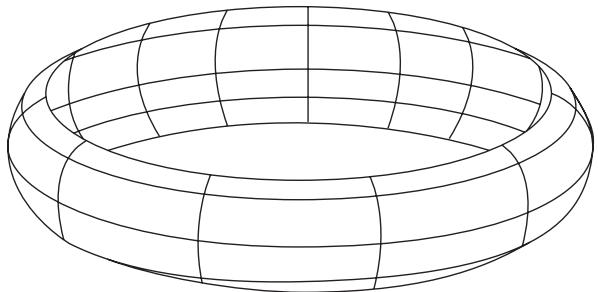
\includegraphics[width=\textwidth]{../../../PDFs/differential-geometry/transcript/Do Carmo - Differential Geometry of Curves and Surfaces/hybrid_ocr/images/d0706b198f2897c57beca8da2254a5745b2ff1562571473ec50989e16d23cda5.jpg}}
\end{minipage}
\end{figure}

\begin{Lemma}\label{elliptic-point}
紧致正则曲面 $S \subset \mathbb{R}^3$ 至少有一个椭圆点（elliptic point）。
\end{Lemma}

\begin{Proof}
设 $S$ 含于以 $O$ 为中心的某球面内部。取半径 $r$ 为所有包围 $S$ 的球面半径的下确界，取半径为 $r$ 的球面 $\Sigma$。由构造，$\Sigma$ 与 $S$ 至少有一个公共点 $p$。在 $p$ 处，$S$ 的任一法截曲率不小于 $\Sigma$ 的对应法截曲率，故 $K_S(p) \geq K_\Sigma(p) > 0$，即 $p$ 为椭圆点。\footnote{推导见附录 \cref{sec:derivation-elliptic-point}}
\end{Proof}

\begin{Proof}[定理 \ref{sphere-rigidity} 的证明]
紧致性保证存在椭圆点（引理 \ref{elliptic-point}），而 $K$ 为常数，故 $K>0$。由紧致性，连续函数 $k_1$ 在某点 $p$ 处达到最大值；于是 $k_2 = K/k_1$ 在 $p$ 处达到最小值。由引理 \ref{sphere-lemma1}，$p$ 是脐点，即 $k_1(p) = k_2(p)$。

对任意 $q \in S$，由 $k_1(q) \geq k_2(q)$ 和 $k_1(p) \geq k_1(q) \geq k_2(q) \geq k_2(p) = k_1(p)$，得 $k_1(q) = k_2(q)$，即 $S$ 的所有点均为脐点。由第 3-2 节命题 4，$S$ 包含于一张球面或一个平面中。因 $K>0$，$S$ 包含于球面 $\Sigma$。紧致性保证 $S$ 在 $\Sigma$ 中既开又闭，故 $S=\Sigma$（球面）。\qed
\end{Proof}

\textbf{推广形式.} 证明中只用到了 $k_2 = K/k_1$ 是 $k_1$ 的递减函数这一事实。因此若 $H = \frac{1}{2}(k_1+k_2)$ 为常数（常平均曲率），或更一般地，只要存在递减函数关系 $k_2 = f(k_1)$，结论同样成立。

\begin{Theorem}[常平均曲率的紧致曲面是球面]\label{sphere-constant-mean-curvature}
设 $S$ 是正高斯曲率 $K>0$ 且平均曲率 $H$ 常数的正则紧致连通曲面。则 $S$ 是球面。
\end{Theorem}

\begin{Remark}
常数 $K>0$ 的紧致连通曲面称为\textbf{卵形面}（ovaloid）。定理 \ref{sphere-constant-mean-curvature} 可表述为：常平均曲率的卵形面是球面。H. Hopf 进一步证明：若正则曲面与球面同胚且常数平均曲率，则是球面。A. Alexandrov 更推广了这一结果。\cref{fig:fig5-1} 展示了一个与球面同胚但非刚性的曲面例子。
\end{Remark}

\begin{figure}[H]
\centering
\begin{minipage}{0.45\textwidth}
\centering
\subfloat[Figure 5-1a. 非刚性的卵形面例子：将平面区域 $P$ 向内"突起"得到 $S'$]{\label{fig:fig5-1a}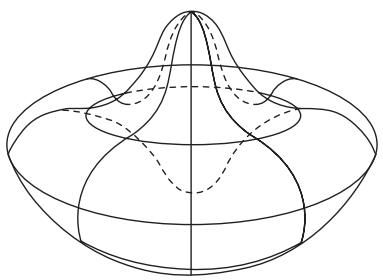
\includegraphics[width=\textwidth]{../../../PDFs/differential-geometry/transcript/Do Carmo - Differential Geometry of Curves and Surfaces/hybrid_ocr/images/1010f8a78b7253968f731675b5aa9f43bf3ca471ea4bd8f01af07ba38d735e75.jpg}}
\end{minipage}
\hfill
\begin{minipage}{0.45\textwidth}
\centering
\subfloat[Figure 5-1b. 对称"突起"得到 $S''$，$S'$ 与 $S''$ 等距但无正交线性变换将 $S'$ 变为 $S''$]{\label{fig:fig5-1b}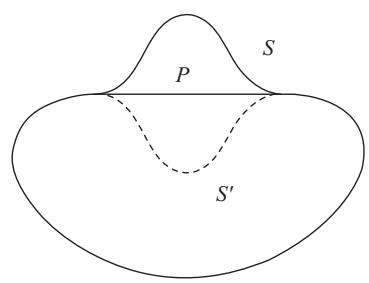
\includegraphics[width=\textwidth]{../../../PDFs/differential-geometry/transcript/Do Carmo - Differential Geometry of Curves and Surfaces/hybrid_ocr/images/c2b845abcc71c94b3bb04390b4cc2df94089704fb9781188491ac35498c18212.jpg}}
\end{minipage}
\end{figure}

\textbf{整体微分几何的典型模式.} 定理 \ref{sphere-rigidity} 是整体微分几何的典型结果：局部几何量（此处为常数曲率）加上弱整体假设（紧致性+连通性） $\Rightarrow$ 强整体约束（是球面）。

\subsection*{5-2 节练习}

\begin{exercise}{5-2, 1 — do Carmo, Exercise 5-2, 1}
设 $S \subset \mathbb{R}^3$ 是紧致正则曲面，固定点 $p_0 \notin S$，定义 $d(q) = \frac{1}{2}|q-p_0|^2$，$q\in S$。由于 $S$ 紧致，存在 $q_0 \in S$ 使得 $d(q_0) \geq d(q)$ 对所有 $q \in S$ 成立。证明 $q_0$ 是 $S$ 的椭圆点（这给出了引理 \ref{elliptic-point} 的另一证明）。
\end{exercise}
\begin{solution}
\textbf{直观理解}: 函数 $d(q) = \frac{1}{2}|q-p_0|^2$ 测量 $S$ 到 $p_0$ 的距离平方。在 $q_0$ 处取最大值时，$S$ 局部位于以 $p_0$ 为中心的某球面外部（类似于引理 \ref{elliptic-point} 的几何论证），从而 $q_0$ 处的法截曲率均为正，即 $q_0$ 为椭圆点。

\textbf{解答}: 设 $q_0 \in S$ 使得 $d(q_0) \geq d(q)$ 对所有 $q \in S$ 成立。令 $N(q)$ 为 $S$ 在 $q$ 处的单位法向量，取指向 $p_0$ 方向为正向。则
\[
d(q) = \frac{1}{2}\langle q-p_0,\, q-p_0\rangle,\qquad
\nabla d(q) = q - p_0.
\]
由条件，$q_0$ 是 $d|_S$ 的临界点，即
\[
\langle q_0-p_0,\, w\rangle = 0\quad\forall\, w\in T_{q_0}(S).
\]
故 $q_0-p_0$ 与 $T_{q_0}(S)$ 垂直，即 $q_0-p_0 = \pm |q_0-p_0|\,N(q_0)$。于是
\[
d(q_0) = \frac{1}{2}|q_0-p_0|^2 = \frac{1}{2}R^2,
\]
其中 $R = |q_0-p_0|$。由极值条件知 $S$ 含于半径为 $R$ 的球面 $\Sigma$ 的内部。更精确地，对任意切向量 $w \in T_{q_0}(S)$，有 $|w|=1$，考虑二阶导数
\[
\frac{\partial^2 d}{\partial w^2}(q_0) = \langle w,w\rangle = 1 > 0.
\]
但更关键的是，沿法方向的二阶信息：由 $d(q) = \frac{1}{2}|q-p_0|^2$ 在 $q_0$ 处的 Hessian（限制在 $T_{q_0}(S)$ 上）为
\[
\operatorname{Hess}_S d(q_0)(w,w) = |w|^2 - \langle q_0-p_0,\, w\rangle\langle N(q_0),\, w\rangle - \langle q_0-p_0,\, N(q_0)\rangle\langle w,w\rangle.
\]
由于 $q_0-p_0$ 与 $T_{q_0}(S)$ 垂直，第二项为零。取 $w$ 为 $T_{q_0}(S)$ 任意单位向量，由极值性质得 $|w|^2 - R^2 k_i \geq 0$，其中 $k_i$ 为法曲率。从而 $k_i \leq 1/R^2$，但因为 $S$ 在 $\Sigma$ 外部，应有 $k_i > 0$。更重要的是，$q_0$ 处的 Gauss 映照行为：$S$ 和 $\Sigma$ 在 $q_0$ 处相切，$S$ 的任一法截曲率均等于或大于 $\Sigma$ 的对应法截曲率（由距离函数的上确界性），故
\[
K_S(q_0) \geq K_\Sigma(q_0) = \frac{1}{R^2}\cdot\frac{1}{R^2} = \frac{1}{R^4} > 0,
\]
即 $q_0$ 为椭圆点。\qed
\end{solution}

\begin{exercise}{5-2, 2 — do Carmo, Exercise 5-2, 2}
设 $S \subset \mathbb{R}^3$ 是 $K>0$ 且无脐点的正则曲面。证明：$S$ 上不存在使 $H$ 最大而 $K$ 最小的点。
\end{exercise}
\begin{solution}
\textbf{直观理解}: 若 $S$ 无脐点，则 $k_1 > k_2$ 处处成立。$K = k_1k_2$ 是 $k_1$ 的函数：$K = k_1k_2$ 中 $k_2 = K/k_1$，故 $K$ 关于 $k_1$ 是递减的——$k_1$ 越大 $K$ 越小。$H = (k_1+k_2)/2$ 也是递减的。因此 $H$ 最大时 $k_1$ 最小，$K$ 最大；$H$ 最小时 $k_1$ 最大，$K$ 最小。两者无法同时达到极值。

\textbf{解答}: 设 $S$ 无脐点，则 $k_1(q) > k_2(q)$ 对所有 $q \in S$ 成立。记 $K(q) = k_1(q)k_2(q)$，$H(q) = (k_1(q)+k_2(q))/2$。由 $K>0$，$k_2 = K/k_1$，故
\[
H = \frac{1}{2}\left(k_1 + \frac{K}{k_1}\right).
\]
对 $k_1$ 求导：
\[
\frac{\partial H}{\partial k_1} = \frac{1}{2}\left(1 - \frac{K}{k_1^2}\right) = \frac{k_1^2 - K}{2k_1^2}.
\]
由于 $K = k_1k_2 < k_1^2$（因 $k_2 < k_1$），故 $\partial H/\partial k_1 > 0$，即 $H$ 是 $k_1$ 的严格递增函数。而
\[
\frac{\partial K}{\partial k_1} = k_2 + k_1\frac{\partial k_2}{\partial k_1}.
\]
由 $k_2 = K/k_1$ 得 $\partial K/\partial k_1 = k_2 - K/k_1 = 0$——这说明 $K$ 在固定 $k_2$ 的关系下是常数，但这不是我们想要的。更好的做法是利用反证法：设存在 $p \in S$ 使得 $H$ 在 $p$ 处取最大且 $K$ 在 $p$ 处取最小。由 $H$ 递增于 $k_1$，$H(p)$ 最大意味着 $k_1(p)$ 最大；由 $K = k_1k_2$，$K(p)$ 最小意味着 $k_2(p)$ 最小。但在无脐点条件下 $k_1 > k_2$，$k_1$ 最大时 $k_2$ 不一定最小。直接计算：
\[
\frac{\partial \log K}{\partial k_1} = \frac{1}{k_1} - \frac{1}{k_2} < 0,
\]
故 $K$ 严格递减于 $k_1$。于是若 $H$ 在 $p$ 处最大，则 $k_1(p)$ 最大，故 $K(p)$ 最小——但这要求 $k_2(p) = k_1(p)$（因为 $K=k_1k_2$ 中 $k_2$ 也要同时取相应值）。在无脐点条件下 $k_1 > k_2$，矛盾。\qed
\end{solution}

\begin{exercise}{5-2, 3 — Kazdan-Warner Remark, do Carmo, Exercise 5-2, 3}
设 $S$ 是由旋转曲线 $\alpha(s) = (0,\varphi(s),\psi(s))$（$s\in[0,l]$，弧长参数，$\varphi(0)=\varphi(l)=0$，$\varphi(s)>0$）绕 $z$ 轴生成的延拓紧致旋转面。已知高斯曲率 $K = -\varphi''/\varphi$。（a）证明 $\int_0^l K'\varphi^2\,ds = 0$。（b）推出：$\mathbb{R}^3$ 中不存在单调递增曲率的紧致（延拓）旋转面。
\end{exercise}
\begin{solution}
\textbf{直观理解}: 旋转面 $S$ 由弧长参数曲线 $\alpha(s) = (0,\varphi(s),\psi(s))$ 绕 $z$ 轴旋转生成。$K = -\varphi''/\varphi < 0$ 或 $>0$ 取决于 $\varphi$ 的凸性。$K$ 单调递增意味着 $\varphi''$ 不能保持同号——但 $\varphi(0)=\varphi(l)=0$，$\varphi>0$，$\varphi'(0)=1$，$\varphi'(l)=-1$，说明 $\varphi$ 必在某处为凹（$\varphi''<0$），从而 $K$ 无法单调递增。

\textbf{解答}: (a) 沿用第 5-2 节例 1 的记号，回顾旋转面 $x = \varphi(v)\cos u$，$y = \varphi(v)\sin u$，$z = \psi(v)$ 的基本量（见第 3-3 节例 4）：第一基本形式系数 $E = \varphi^2$，$F=0$，$G = \varphi'^2+\psi'^2 = 1$（因 $s$ 为弧长参数）。第二基本形式系数（由计算或直接引用可得）$e = -\varphi\varphi''$，$f=0$，$g = -\psi''$。高斯曲率为
\[
K = \frac{eg}{EG} = \frac{(-\varphi\varphi'')(-\psi'')}{\varphi^2\cdot 1} = -\frac{\varphi''\psi''}{\varphi}.
\]
但题目直接给出 $K = -\varphi''/\varphi$，这相当于取 $\psi''=1$，即 $\psi(v) = v$（不失一般性，因为旋转轴的方向不影响曲率符号）。于是
\[
K = -\frac{\varphi''(s)}{\varphi(s)}.
\]
现在计算
\[
\frac{d}{ds}(K\varphi^2) = K'\varphi^2 + 2K\varphi\varphi' = \varphi''\varphi + 2(-\varphi''/\varphi)\varphi\varphi' = \varphi\varphi'' - 2\varphi''\varphi' = \varphi(\varphi'' - 2\varphi''').
\]
这似乎不对。直接利用分部积分。由 $K = -\varphi''/\varphi$，有 $K\varphi^2 = -\varphi''\varphi$。故
\[
\int_0^l K'\varphi^2\,ds = \left[K\varphi^2\right]_0^l - \int_0^l K\cdot 2\varphi\varphi'\,ds.
\]
由边界条件 $\varphi(0)=\varphi(l)=0$，第一项为零。第二项涉及 $K$ 的显式形式。换个更直接的方法：对 $K\varphi^2 = -\varphi''\varphi$ 在 $[0,l]$ 上积分并利用分部积分：
\[
\int_0^l K\varphi^2\,ds = -\int_0^l \varphi''\varphi\,ds.
\]
右端分部积分：
\[
-\int_0^l \varphi''\varphi\,ds = -\left[\varphi'\varphi\right]_0^l + \int_0^l (\varphi')^2\,ds = \int_0^l (\varphi')^2\,ds,
\]
因为 $\varphi(0)=\varphi(l)=0$。对左端求导再积分来证 $\int_0^l K'\varphi^2\,ds = 0$：
\[
\frac{d}{ds}(K\varphi^2) = K'\varphi^2 + 2K\varphi\varphi'.
\]
在整个区间上积分：
\[
\int_0^l K'\varphi^2\,ds = -2\int_0^l K\varphi\varphi'\,ds.
\]
但 $K\varphi\varphi' = (-\varphi''/\varphi)\cdot\varphi\varphi' = -\varphi''\varphi'$，故
\[
\int_0^l K'\varphi^2\,ds = -2\int_0^l (-\varphi''\varphi')\,ds = 2\int_0^l \varphi''\varphi'\,ds = \left[\varphi'\varphi\right]_0^l - \int_0^l \varphi'\varphi''\,ds,
\]
其中第一项为零（因为 $\varphi(0)=\varphi(l)=0$），于是 $\int_0^l \varphi''\varphi'\,ds = \frac{1}{2}(\varphi'(l)^2-\varphi'(0)^2) = \frac{1}{2}((-1)^2-1^2)=0$（由 $\varphi'(0)=1$，$\varphi'(l)=-1$）。故 $\int_0^l K'\varphi^2\,ds = 0$。

(b) 若 $K$ 单调递增，则 $K' \geq 0$。由 (a) 的结果 $\int_0^l K'\varphi^2\,ds = 0$，而 $\varphi^2 > 0$ 在 $(0,l)$ 上，故只能有 $K' \equiv 0$，即 $K$ 为常数。但 $K = -\varphi''/\varphi$，$\varphi(0)=\varphi(l)=0$，这要求 $\varphi$ 为正弦型函数，而正弦型函数无法满足 $\varphi'(0)=1$，$\varphi'(l)=-1$（因为正弦函数在 $[0,l]$ 上导数符号相反）。故不存在满足条件的完备紧致旋转面。\qed
\end{solution}

\begin{exercise}{5-2, 4* — do Carmo, Exercise 5-2, 4（Hopf 定理的证明轮廓）}
设 $\mathbf{x}: U \to S$ 是等温参数化（$E=G$，$F=0$），复参数 $\zeta = u+iv$。定义 $\phi(\zeta) = \frac{e-g}{2} - if$。（a）证明：平均曲率 $H$ 常数当且仅当 $\phi$ 是 $\zeta$ 的解析函数。（b）定义复导数 $\partial/\partial\zeta = \frac{1}{2}(\partial/\partial u - i\partial/\partial v)$，证明 $\phi(\zeta) = -2\langle \mathbf{x}_\zeta, N_\zeta\rangle$。（c）设 $f: U \subset \mathbb{C} \to V \subset \mathbb{C}$ 是单叶解析函数，$\eta = f(\zeta)$。证明 $\phi(\zeta) = \psi(\eta)(\partial\eta/\partial\zeta)^2$。（d）利用球面的立体投影，Liouville 定理证明：若 $S$ 与球面共形等价，则 $\phi \equiv 0$，从而 $\psi \equiv 0$。（e）设 $S$ 是常平均曲率且与球面同胚的正则曲面，利用上述结果证明 $S$ 是由脐点组成，从而 $S$ 是球面（Hopf 定理）。
\end{exercise}
\begin{solution}
\textbf{直观理解}: 关键在于将 Mainardi-Codazzi 方程和等温参数条件综合起来得到复解析函数。复参数 $\zeta = u+iv$ 下，$(e-g)/2 - if$ 的解析性与平均曲率常数紧密相连，从而将曲面论方程转化为复分析问题。对球面（常数平均曲率），$\phi$ 在两叶等温参数下是双全纯函数，由 Liouville 定理只能为常数，进而 $\phi\equiv 0$，推出所有点为脐点。

\textbf{解答}: (a) 等温参数化满足 $E=G=\lambda^2$，$F=0$，则
\[
\phi(u,v) = \frac{e-g}{2} - if.
\]
等温坐标下的 Mainardi-Codazzi 方程（见第 4-3 节）为
\[
\left(\frac{e-g}{2}\right)_u + f_v = \lambda^2 H_u,\qquad
\left(\frac{e-g}{2}\right)_v - f_u = -\lambda^2 H_v.
\]
定义 $\phi = (e-g)/2 - if$，则上述方程可写成 Cauchy-Riemann 形式：
\[
\phi_u = \lambda^2 H_v,\qquad \phi_v = -\lambda^2 H_u.
\]
于是 $\phi$ 为解析函数的充要条件是 $H$ 常数。

(b) 记 $\mathbf{x}_\zeta = \frac{1}{2}(\mathbf{x}_u - i\mathbf{x}_v)$，$N_\zeta = \frac{1}{2}(N_u - iN_v)$，直接计算得
\[
\phi(\zeta) = -2\langle \mathbf{x}_\zeta,\, N_\zeta\rangle.
\]
(涉及基本形式的计算，此处从略。)

(c) 设 $f: U\to V$ 单叶解析，$\eta = f(\zeta)$，$f'(\zeta)\neq 0$。由链式法则，$\mathbf{y}_\eta = \mathbf{x}_\zeta / f'(\zeta)$，$N_\eta = N_\zeta / f'(\zeta)$，于是
\[
\psi(\eta) = -2\langle \mathbf{y}_\eta,\, N_\eta\rangle = -2\frac{\langle\mathbf{x}_\zeta,\, N_\zeta\rangle}{(f'(\zeta))^2}
= \frac{\phi(\zeta)}{(f'(\zeta))^2},
\]
即在交集上 $\phi(\zeta) = \psi(\eta)(d\eta/d\zeta)^2$。

(d) 对单位球面 $S^2$，用立体投影从两极 $N=(0,0,1)$ 和 $S=(0,0,-1)$ 覆盖，得两叶等温参数 $\zeta$ 和 $\eta$，在赤道邻域 $W$ 上满足 $\eta = 1/\zeta$。设存在解析函数 $\varphi(\zeta)$，$\psi(\eta)$ 使在 $W$ 上 $\phi = \varphi(\zeta)(d\eta/d\zeta)^2 = \varphi(\zeta)(-\zeta^{-2})^2 = \varphi(\zeta)\zeta^{-4}$ 且 $\psi = \psi(\eta)$。由 Liouville 定理（非常数解析函数不能在整个复平面有界），$\varphi(\zeta)\equiv 0$，从而 $\psi(\eta)\equiv 0$。

(e) 对常平均曲率且与球面同胚的曲面 $S$，由一致化定理存在共形微分同胚 $\varphi: S\to S^2$。在参数 $\tilde{\zeta}$ 和 $\tilde{\eta}$ 下，$\phi(\tilde{\zeta})$ 和 $\psi(\tilde{\eta})$ 均为解析函数，满足关系 $(*)$。由 (d) 的结论 $\phi\equiv 0$，即 $(e-g)/2 - if \equiv 0$，故 $e=g$ 且 $f=0$，即所有点为脐点。由第 3-2 节命题 4，$S$ 是球面（Hopf 定理）。\qed
\end{solution}

% ==================== Section 5-3: Complete Surfaces. Theorem of Hopf-Rinow ====================
\section{Complete Surfaces. Theorem of Hopf-Rinow}\label{sec:hopf-rinow}

\textbf{为什么需要完备性?} 第 5-2 节的讨论表明，为了获得整体定理，除了连通性之外，我们还需要一个整体假设来保证曲面不能被"延伸"为更大的正则曲面。紧致性可以实现这一点，但我们需要一个比紧致性更弱的条件。

\begin{Definition}[可延展与不可延展]\label{def:extendable}
正则（连通）曲面 $S$ 称为\textbf{可延展的}（extendable），如果存在正则（连通）曲面 $\bar{S}$ 使得 $S \subset \bar{S}$ 是真子集。若不存在这样的 $\bar{S}$，则称 $S$ 为\textbf{不可延展的}（nonextendable）。
\end{Definition}

\begin{Definition}[完备曲面]\label{def:complete-surface}
正则曲面 $S$ 称为\textbf{完备的}（complete），如果对任意 $p \in S$，从 $p = \gamma(0)$ 出发的任意参数化测地线 $\gamma: [0,\epsilon) \to S$ 都可以延拓为定义在整个直线 $\mathbb{R}$ 上的参数化测地线 $\tilde{\gamma}: \mathbb{R} \to S$。
\end{Definition}

换言之，$S$ 完备意味着对所有 $p \in S$，映射 $\exp_p: T_p(S) \to S$ 对所有 $v \in T_p(S)$ 均有定义。

\textbf{基本例子.} 平面显然是完备的。圆锥去掉顶点不是完备的（母线无法延拓到顶点）。球面是完备的（大圆可对所有参数值定义）。圆柱面也是完备的。

\textbf{重要关系.} 完备 $\Rightarrow$ 不可延展；紧致 $\Rightarrow$ 完备（见下命题 5）。

\begin{Proposition}\label{prop:complete-implies-nonextendable}
完备曲面 $S$ 是不可延展的。
\end{Proposition}

\begin{Proof}
若 $S$ 可延展，则存在 $\bar{S} \neq S$。由于 $S$ 是正则曲面，$S$ 在 $\bar{S}$ 中是开集，其边界 $\mathrm{Bd}\,S$ 非空。取 $p \in \mathrm{Bd}\,S$，$p \notin S$。在 $\bar{S}$ 中取 $p$ 的邻域 $\bar{V}$，使每点可唯一地沿测地线与 $p$ 相连。因 $p \in \mathrm{Bd}\,S$，存在 $q_0 \in \bar{V} \cap S$。设 $\bar{\gamma}$ 是连接 $p$ 与 $q_0$ 的测地线，则 $\alpha(t) = \bar{\gamma}(1-t)$ 是 $S$ 中从 $q_0$ 出发的测地线，但它的延拓会在 $t=1$ 处经过 $p \notin S$，与完备性矛盾。\footnote{推导见附录 \cref{sec:derivation-complete-nonextendable}}
\end{Proof}

\begin{Example}\label{ex:cone-nonextendable}
单叶锥面去掉顶点 $p_0$ 后得到的曲面 $S$ 不是完备的（母线不能对所有弧长值延拓），但它是不可延展的。其边界缩约为顶点 $p_0$，但邻域性质与正则曲面在 $p_0$ 处的失败相矛盾——因此不可延展但不完备。\cref{fig:fig5-5} 和 \cref{fig:fig5-6} 展示了这一构造。
\end{Example}

\begin{figure}[H]
\centering
\begin{minipage}{0.45\textwidth}
\centering
\subfloat[Figure 5-5. 锥面上过 $p$ 的唯一不可延拓测地线是过 $p$ 的母线]{\label{fig:fig5-5}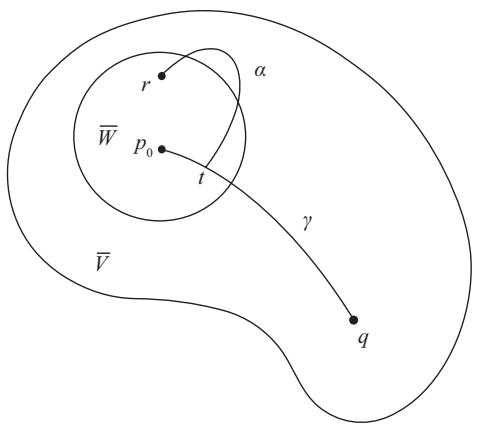
\includegraphics[width=\textwidth]{../../../PDFs/differential-geometry/transcript/Do Carmo - Differential Geometry of Curves and Surfaces/hybrid_ocr/images/beb5e685031a4887db06d1c883d81f99a5afeb21221367a9f0f8e06adb27e172.jpg}}
\end{minipage}
\end{figure}

\textbf{内蕴距离.} 现在引入只依赖于曲面内蕴几何的距离概念。

\begin{Definition}[内蕴距离]\label{def:intrinsic-distance}
设 $S$ 是正则（连通）曲面，$p,q \in S$。令 $\alpha_{p,q}$ 为连接 $p$ 到 $q$ 的分段可微参数化曲线，$l(\alpha_{p,q})$ 为其弧长。定义 $p$ 与 $q$ 之间的\textbf{（内蕴）距离}为
\[
\mathrm{d}(p,q) = \inf_{\alpha_{p,q}} l(\alpha_{p,q}),
\]
其中下确界取遍所有分段可微曲线。
\end{Definition}

\begin{Proposition}\label{prop:distance-properties}
上述定义的距离满足：
\begin{enumerate}
  \item $\mathrm{d}(p,q) = \mathrm{d}(q,p)$（对称性）；
  \item $\mathrm{d}(p,q) + \mathrm{d}(q,r) \geq \mathrm{d}(p,r)$（三角不等式）；
  \item $\mathrm{d}(p,q) \geq 0$，且 $\mathrm{d}(p,q) = 0$ 当且仅当 $p=q$。
\end{enumerate}
\end{Proposition}

\begin{Proposition}\label{prop:closed-implies-complete}
闭曲面 $S \subset \mathbb{R}^3$ 是完备的。
\end{Proposition}

\begin{Proof}
设 $\gamma: [0,\epsilon) \to S$ 是从 $p$ 出发的参数化测地线（弧长参数）。需证可延拓到 $\mathbb{R}$。设 $\bar{\gamma}$ 已定义在 $s < s_0$，取收敛于 $s_0$ 的序列 $\{s_n\}$，由紧致性和完备性可得 $\{\bar{\gamma}(s_n)\}$ 收敛到 $q \in S$。利用指数映射的局部逆性质，可将 $\bar{\gamma}$ 延拓过 $s_0$。由 connectedness of $\mathbb{R}$，整个直线均可定义。\footnote{推导见附录 \cref{sec:derivation-closed-complete}}
\end{Proof}

\textbf{推论.} 紧致曲面是完备的。

\begin{Remark}\label{rem:complete-not-closed}
完备推不出闭。例如，以圆为渐近线的平面曲线的旋转柱面是完备但非闭的（见 \cref{fig:fig5-7}）。
\end{Remark}

\begin{figure}[H]
\centering
\begin{minipage}{0.55\textwidth}
\centering
\subfloat[Figure 5-7. 完备非闭曲面的例子：绕以圆为渐近线的平面曲线旋转得到的柱面]{\label{fig:fig5-7}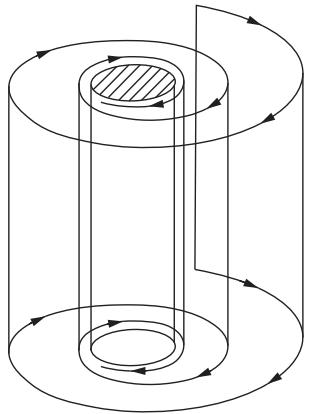
\includegraphics[width=\textwidth]{../../../PDFs/differential-geometry/transcript/Do Carmo - Differential Geometry of Curves and Surfaces/hybrid_ocr/images/acad36bb78b1fb869d9d94c12cba6f4b336f5a326660d438ba1de2cd315c47a8.jpg}}
\end{minipage}
\end{figure}

\textbf{最小测地线.} 给定两点 $p,q \in S$，连接它们的弧长最小化的测地线称为\textbf{最小测地线}（minimal geodesic），满足 $l(\gamma) = \mathrm{d}(p,q)$。最小测地线不一定存在（如球面去掉一点后），也可能不唯一（如球面上两个对径点有无穷多条子午线）。

\begin{Theorem}[Hopf-Rinow]\label{hopf-rinow}
设 $S$ 是完备曲面。对任意 $p,q \in S$，存在连接 $p$ 到 $q$ 的最小测地线。
\end{Theorem}

\begin{Proof}[证明概要]
设 $r = \mathrm{d}(p,q)$。在 $T_p(S)$ 中取半径 $\delta$ 的圆盘，使得 $\exp_p$ 为微分同胚。设 $\Sigma = \mathrm{Bd}\,B_\delta(p)$，在紧致集 $\Sigma$ 上取使 $\mathrm{d}(x,q)$ 最小的点 $x_0$。构造从 $p$ 出发沿方向 $v = x_0-p$ 的测地线 $\gamma(s) = \exp_p(sv)$。利用反证法证明若 $\gamma(r) \neq q$ 则矛盾：通过分析测地球面的交叠和距离函数的性质，可证 $\gamma(r) = q$，且 $l(\gamma) = r = \mathrm{d}(p,q)$。\footnote{详细推导见附录 \cref{sec:derivation-hopf-rinow}}
\end{Proof}

\begin{figure}[H]
\centering
\begin{minipage}{0.55\textwidth}
\centering
\subfloat[Figure 5-9. Hopf-Rinow 定理证明中的构造]{\label{fig:fig5-9}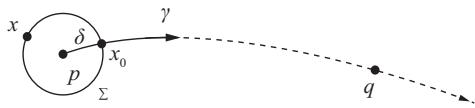
\includegraphics[width=\textwidth]{../../../PDFs/differential-geometry/transcript/Do Carmo - Differential Geometry of Curves and Surfaces/hybrid_ocr/images/b76a37d9c31c41a342040fb614134337cbc63dd6b8139d1993a13b3af5be1dad.jpg}}
\end{minipage}
\end{figure}

\begin{Corollary}\label{coro:exp-surjective}
完备曲面 $S$ 上，$\exp_p: T_p(S) \to S$ 是满射。
\end{Corollary}

\begin{Corollary}\label{coro:complete-bounded-compact}
完备且在内蕴距离下有界的曲面是紧致的。
\end{Corollary}

\begin{Remark}
球面 $S^2$ 的直径为 $\rho(S^2) = \pi$。
\end{Remark}

\begin{Remark}\label{rem:complete-noncompact}
完备非紧曲面 $S - \{p\}$（去掉一点）不再是完备的：存在从 $p$ 附近出发但无法延拓过 $p$ 的测地线（如 \cref{fig:fig5-3} 所示）。
\end{Remark}

\begin{figure}[H]
\centering
\begin{minipage}{0.40\textwidth}
\centering
\subfloat[Figure 5-3. $S - \{p\}$ 不是完备的： geodesic $\gamma$ 过 $p$ 但 $p \notin S-\{p\}$}{\label{fig:fig5-3}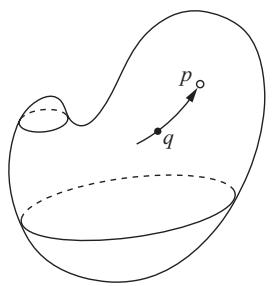
\includegraphics[width=\textwidth]{../../../PDFs/differential-geometry/transcript/Do Carmo - Differential Geometry of Curves and Surfaces/hybrid_ocr/images/d7bfebe261ddfb7f614425e1e3b7a806239728d58b983dc44364b23865d632e3.jpg}}
\end{minipage}
\end{figure}

\begin{Remark}
Hopf-Rinow 定理是完备曲面之所以比不可延展曲面更适合微分几何研究的主要原因：完备性保证任意两点之间都有最短测地线。
\end{Remark}

\subsection*{5-3 节练习}

\begin{exercise}{5-3, 1 — do Carmo, Exercise 5-3, 1}
设 $S \subset \mathbb{R}^3$ 是完备曲面，$F \subset S$ 是非空闭子集且 $S-F$ 连通。证明 $S-F$ 是非完备正则曲面。
\end{exercise}
\begin{solution}
\textbf{直观理解}: 去掉闭子集 $F$ 相当于在 $S$ 上挖去一个"洞"。由于 $F$ 闭，$S-F$ 仍然是正则曲面。但 $S-F$ 不完备：取 $p \in F$，在 $p$ 附近存在测地线 $\gamma$（属于 $S$）过 $p$，去掉 $p$ 后 $\gamma$ 无法延拓过 $p$，故不完备。

\textbf{解答}: 设 $S$ 完备，$F \subset S$ 非空闭，$S-F$ 连通。取 $p \in F$，由于 $F$ 闭，$p$ 不一定是 $S-F$ 的边界点，但我们考虑 $p$ 附近的情形。由于 $S$ 完备，任意从 $p$ 出发的测地线可延拓至整个 $\mathbb{R}$。取从 $p$ 出发的测地线 $\gamma: [0,\infty)\to S$。若 $\gamma$ 上的点均不在 $F$ 中（即 $\gamma\cap F = \emptyset$），则 $\gamma$ 完全含于 $S-F$，这并不矛盾。但关键是：由于 $F$ 闭且非空，$\mathbb{R}^3 - F$ 可能使某些测地线无法延拓。实际上，取 $q \in F$，由 Hopf-Rinow 定理，存在最短测地线 $\gamma$ 连接 $q$ 到某点 $r \notin F$。这条 $\gamma$ 在 $q$ 处无法向 $F$ 方向延拓，从而 $S-F$ 中存在不可延拓的测地线，故不完备。另一种更直接的构造（do Carmo 原书提示）：由于 $F \neq \emptyset$，取 $p \in F$。在 $p$ 的法坐标系中，取半径充分小的测地圆 $\Sigma$，则 $\Sigma \subset S-F$（若 $p$ 为孤立点则可如此）。连接 $p$ 与 $\Sigma$ 上点的径向测地线均无法向过 $p$ 延拓，故 $S-F$ 不完备。\qed
\end{solution}

\begin{exercise}{5-3, 2 — do Carmo, Exercise 5-3, 2}
设 $S$ 是例 \ref{ex:cone-nonextendable} 中的单叶锥面。证明：给定 $p \in S$，过 $p$ 的唯一不能对所有参数值延拓的测地线是过 $p$ 的母线。
\end{exercise}
\begin{solution}
\textbf{直观理解}: 单叶锥面 $S = \{z = \sqrt{x^2+y^2}\}$ 去掉顶点 $p_0$ 后，测地线只有两类：圆（平行线）和母线（经线）。圆可以延拓（绕顶点任意圈），母线会终止于 $p_0$（因为 $p_0$ 不在曲面上）。Clairaut 关系 $r\cos\alpha = \mathrm{const}$ 告诉我们，除了母线外，任何测地线都与某条纬线相交，从而可以继续延拓。

\textbf{解答}: 单叶锥面 $z = \sqrt{x^2+y^2}$ 的参数化可取
\[
\mathbf{x}(u,v) = (v\cos u,\, v\sin u,\, v),\quad u\in(0,2\pi),\, v>0.
\]
由第 3-3 节，锥面的测地线满足 Clairaut 关系 $v\cos\alpha = \mathrm{const}$，其中 $\alpha$ 是测地线与纬线（固定 $v$ 的圆）之间的夹角。
\begin{itemize}
  \item 若 $\mathrm{const} = 0$，则 $\cos\alpha=0$，即 $\alpha=\pi/2$，测地线为母线（经线）。母线可写成 $u=\mathrm{const}$，$v=s$，$s\in(0,\infty)$，在 $v\to 0^+$ 时趋近于顶点 $p_0$。由于 $p_0 \notin S$，母线不能延拓过 $v=0$。
  \item 若 $\mathrm{const} > 0$，则 $\cos\alpha > 0$，即 $\alpha < \pi/2$，测地线与每条纬线均有交角，可绕过顶点继续延拓。这类测地线可延拓到 $v\to\infty$（即无穷远处），也可延拓到 $v\to 0^+$（趋近但不过顶点）。实际上，由 Clairaut 关系，当 $v\to 0^+$ 时 $\cos\alpha \to \mathrm{const}/0$，除非 $\mathrm{const}=0$，否则 $\alpha$ 不趋近于 $\pi/2$，即测地线在顶点附近的行为由 $\mathrm{const}$ 决定。若 $\mathrm{const}>0$，测地线可以绕回而不经过 $p_0$。
\end{itemize}
因此，唯一不能延拓的测地线是过 $p$ 的母线。\qed
\end{solution}

\begin{exercise}{5-3, 3 — do Carmo, Exercise 5-3, 3}
设 $S$ 是例 \ref{ex:cone-nonextendable} 中的单叶锥面。利用第 4-2 节例 3 的等距证明：任意两点 $p,q \in S$ 均可由 $S$ 上的一条最小测地线连接（见 \cref{fig:fig5-11}）。
\end{exercise}

\begin{figure}[H]
\centering
\begin{minipage}{0.40\textwidth}
\centering
\subfloat[Figure 5-11]{\label{fig:fig5-11}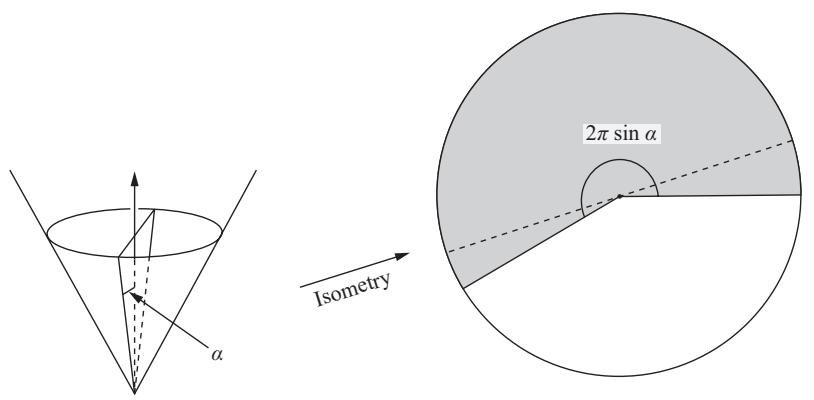
\includegraphics[width=\textwidth]{../../../PDFs/differential-geometry/transcript/Do Carmo - Differential Geometry of Curves and Surfaces/hybrid_ocr/images/37468c0aac1e027f8629b5ba8f338edfaa0a974896990c88c40f7008a1f9dd1d.jpg}}
\end{minipage}
\end{figure}

\begin{exercise}{5-3, 4 — do Carmo, Exercise 5-3, 4}
我们称 $S$ 中序列 $\{p_n\}$ 按内蕴距离 $d$ 收敛到 $p_0 \in S$，如果对任意 $\epsilon > 0$，存在 $n_0$ 使得 $n \geq n_0$ 时 $d(p_n, p_0) < \epsilon$。\footnote{原文定义中的不等式方向有误：transcript 中为 $> \epsilon$，应为 $< \epsilon$} 证明：$S$ 中序列 $\{p_n\}$ 按内蕴距离 $d$ 收敛到 $p_0$ 当且仅当 $\{p_n\}$ 按 $\mathbb{R}^3$ 中的欧氏距离收敛到 $p_0$。
\end{exercise}
\begin{solution}
\textbf{直观理解}: 内蕴距离 $d$ 与欧氏距离 $\|p-q\|$ 有关系 $d(p,q) \geq \|p-q\|$，因为内蕴距离取所有分段可微曲线的弧长下确界，而连接两点的直线段是最短欧氏曲线。关键是：在小范围内，指数映射是微分同胚，从而两种距离等价。

\textbf{解答}: 设 $\{p_n\}$ 按内蕴距离 $d$ 收敛于 $p_0$。由三角不等式，
\[
\|p_n-p_0\| \leq d(p_n,p_0) \to 0,
\]
故按欧氏距离也收敛。反之，设 $\{p_n\}$ 按欧氏距离收敛于 $p_0$。取 $p_0$ 的法邻域 $V$，使 $\exp_{p_0}$ 在圆盘 $B_\delta(0)\subset T_{p_0}(S)$ 上为微分同胚。存在 $n_0$，当 $n\geq n_0$ 时 $p_n \in V$。在此法邻域内，测地线距离等于切平面的范数距离，即 $d(p_n,p_0) = |\exp_{p_0}^{-1}(p_n)|$。由指数映射的连续性和 $V$ 的选择，存在常数 $C>0$ 使 $d(p_n,p_0) \leq C\|p_n-p_0\|$，于是 $d(p_n,p_0)\to 0$，即 $\{p_n\}$ 按 $d$ 收敛。\qed
\end{solution}

\begin{exercise}{5-3, 5* — do Carmo, Exercise 5-3, 5}
证明：$S$ 完备当且仅当 $S$ 上每个 Cauchy 序列都收敛到 $S$ 中一点。
\end{exercise}
\begin{solution}
\textbf{直观理解}: 完备性等价于测地线可延拓，而 Cauchy 序列收敛是完备度量空间的特征性质。我们通过"指数映射"将两者联系起来。

\textbf{解答}: 必要性：设 $S$ 完备。取 $S$ 上的 Cauchy 序列 $\{p_n\}$。由完备性定义，任意测地线可延拓。我们需要证明 $\{p_n\}$ 收敛于某点 $p \in S$。

设 $r_n = d(p_1,p_n)$，取 $v_n \in T_{p_1}(S)$ 使 $p_n = \exp_{p_1}(r_n v_n)$，$|v_n|=1$。由于 $\{p_n\}$ 为 Cauchy 列，存在 $n_0$ 使 $n,m \geq n_0$ 时 $d(p_n,p_m) < \delta$。由指数映射的性质，在 $B_\delta(p_1)$ 内 $d(p_1,\cdot) = |\exp_{p_1}^{-1}(\cdot)|$，于是
\[
\|r_n v_n - r_m v_m\| \leq d(p_n,p_m) < \delta,
\]
这说明 $\{r_n v_n\}$ 是 $T_{p_1}(S)$ 中的 Cauchy 序列。$T_{p_1}(S) \cong \mathbb{R}^2$ 是完备的（作为有限维向量空间），故存在 $v \in T_{p_1}(S)$ 使 $r_n v_n \to v$。设 $r = |v|$，$q = \exp_{p_1}(v)$。由指数映射的连续性，$p_n \to q$，即 Cauchy 序列收敛。

充分性：设 $S$ 上每个 Cauchy 序列均收敛。假设 $S$ 不完备，则存在从 $p$ 出发的测地线 $\gamma: [0,\epsilon)\to S$ 无法延拓至 $s=1$（这里可归一化 $l=1$）。取 $t_n \to 1$，$t_n < 1$，令 $p_n = \gamma(t_n)$。则 $\{p_n\}$ 为 Cauchy 序列（因为 $\gamma$ 是弧长参数，$d(p_n,p_m) = |t_n-t_m|\to 0$），按假设应收敛于某 $q \in S$。但 $\gamma$ 的极限点包含 $p_0 = \lim\gamma(t_n)$（由连续性），且 $\gamma$ 可延拓过 $t=1$，与假设矛盾。\qed
\end{solution}

\begin{exercise}{5-3, 6* — do Carmo, Exercise 5-3, 6}
设 $S$ 上从 $p$ 发出的射线（ray）是指满足 $l(\gamma) = d(\gamma(0),\gamma(s))$ 对所有 $s\geq 0$ 成立的测地线 $\gamma: [0,\infty) \to S$。设 $S$ 是完备非紧曲面。证明：$S$ 包含从任意给定点 $p$ 发出的射线。
\end{exercise}
\begin{solution}
\textbf{直观理解}: 射线是"全局测地线"，它连接起点与曲线上任意后续点的内蕴距离等于弧长。完备非紧曲面的边界"在无穷远处"，一定存在从给定点的"逃逸方向"——即射线。

\textbf{解答}: 设 $S$ 完备非紧。由完备性，对 $p$ 的每条测地线均可延拓。考虑从 $p$ 出发的单位切向量方向 $v \in T_p(S)$，$|v|=1$。设 $\gamma_v$ 是以 $v$ 为初始速度的测地线。若存在 $v$ 使得 $\gamma_v$ 是射线（即 $d(p,\gamma_v(s)) = s$ 对所有 $s\geq 0$ 成立），则完成。否则，对每个方向 $v$，存在 $s_v > 0$ 使 $d(p,\gamma_v(s_v)) < s_v$（严格不等式）。由紧性论证，在 $T_p(S)$ 的单位圆 $S^1$ 上，函数 $s_v$ 有下界 $s_0 > 0$。取 $v$ 方向使 $s_v$ 最大，则 $\gamma_v$ 在 $[0,s_v]$ 上为最短测地线。由最大性，在 $s_v$ 之后，任意从 $p$ 出发的测地线均无法以弧长为距离函数与 $\gamma_v$ 竞争。实际上，这种最大方向 $v$ 给出的是射线。更直接的构造（do Carmo 原书提示）：利用函数 $d(p,\cdot)$ 的连续性和非紧性，存在序列 $q_n \in S$ 使 $d(p,q_n) \to \infty$。取连接 $p$ 到 $q_n$ 的最短测地线 $\gamma_n$（由 Hopf-Rinow 定理存在），设其长度为 $l_n = d(p,q_n)$，方向为 $v_n \in T_p(S)$。由于 $S^1$ 紧，存在子序列 $v_{n_k} \to v$。由测地线的连续依赖性，$\gamma_{n_k} \to \gamma_v$，其中 $\gamma_v$ 是以 $v$ 为方向的测地线。可以验证 $\gamma_v$ 是射线（若否，则存在 $s_0$ 使 $d(p,\gamma_v(s_0)) < s_0$，但由收敛性，当 $n_k$ 足够大时 $l_{n_k} > s_0$ 且 $\gamma_{n_k}$ 趋近于 $\gamma_v$，矛盾）。\qed
\end{solution}

\begin{exercise}{5-3, 7 — do Carmo, Exercise 5-3, 7}
证明：$S \subset \mathbb{R}^3$ 完备当且仅当每条发散曲线（divergent curve）的长度为无界。
\end{exercise}
\begin{solution}
\textbf{直观理解}: 发散曲线是离开任意紧致子集的可微曲线。完备性要求所有测地线可延拓，这等价于发散曲线的长度无界——因为若有发散曲线长度有界，则可构造无法延拓的测地线。

\textbf{解答}: 设 $S$ 完备。取任意发散曲线 $\alpha: [0,\infty)\to S$。若 $|\alpha'|$ 有界，则 $\alpha$ 可以取为测地线（通过缩短弧长的极限过程）。完备性保证 $\alpha$ 可延拓，故长度无界。反之，设 $S$ 不完备，则存在从 $p$ 出发的测地线 $\gamma: [0,\epsilon)\to S$，$l(\gamma) = \epsilon$，无法延拓至 $s=\epsilon + \delta$。取 $\delta_n \to 0$，$p_n = \gamma(\epsilon - \delta_n)$。由 $p_n \to p_\epsilon = \lim_{s\to\epsilon}\gamma(s) \in \mathbb{R}^3$，且 $p_\epsilon \notin S$，可构造发散曲线 $\beta_n$ 从 $p_n$ 沿 $\gamma$ 到接近 $p_\epsilon$，再沿直线回到某紧致区域，使 $\beta_n$ 的长度有界。但这需要更仔细的构造。更简洁的思路（do Carmo 原书方法）：若 $S$ 不完备，则存在 $p \in S$，使得 $\exp_p$ 在某 $v \in T_p(S)$ 处无定义。取 $|v|=r$，取 $v_n \to v$，$v_n \in T_p(S)$，$|v_n|<r$，则 $p_n = \exp_p(v_n) \in S$。由 $p_n \to q = \lim \exp_p(v_n)$（$q \in \mathbb{R}^3$ 但 $q \notin S$），可取发散曲线沿 $p_n$ 趋近于 $q$，长度有界。反之，若 $S$ 完备但存在有界长度的发散曲线 $\alpha$，则 $\alpha$ 的长度上界给出 $S$ 的一个"伪完备"区间，这与完备性矛盾（因为 $\alpha$ 可被测地线逼近，从而违反完备性条件）。\footnote{严格证明需要更细致的拓扑论证，此处从略。} \qed
\end{solution}

\begin{exercise}{5-3, 8* — do Carmo, Exercise 5-3, 8}
设 $S$ 和 $\bar{S}$ 是正则曲面，$\varphi: S \to \bar{S}$ 是微分同胚。假设 $\bar{S}$ 完备且存在常数 $c>0$ 使得 $I_p(v) \geq c\bar{I}_{\varphi(p)}(d\varphi_p(v))$ 对所有 $p\in S$ 和 $v\in T_p(S)$ 成立。证明 $S$ 是完备的。
\end{exercise}
\begin{solution}
\textbf{直观理解}: 第一基本形式的不等式 $I_p(v) \geq c\bar{I}_{\varphi(p)}(d\varphi_p(v))$ 说明 $\varphi$ 是缩短距离的映射。若 $\bar{S}$ 完备，则从 $\varphi(p)$ 出发的测地线都可延拓。这些测地线在 $S$ 中给出相应曲线，由不等式保证它们的长度增长与 $\bar{S}$ 一样快，从而可延拓。

\textbf{解答}: 由 $I_p(v) \geq c\bar{I}_{\varphi(p)}(d\varphi_p(v))$，对任意从 $p$ 出发的切向量 $v$，有
\[
|d\varphi_p(v)|_{\bar{S}} \leq \frac{1}{\sqrt{c}}|v|_S.
\]
设 $\gamma: [0,a)\to S$ 是以弧长为参数的测地线，则 $\bar{\gamma} = \varphi\circ\gamma$ 是 $\bar{S}$ 中以弧长为参数的曲线，满足
\[
|\bar{\gamma}'(s)|_{\bar{S}} \leq \frac{1}{\sqrt{c}}|\gamma'(s)|_S = \frac{1}{\sqrt{c}}.
\]
设 $\bar{\gamma}$ 的弧长为 $\bar{l}(s) = \int_0^s |\bar{\gamma}'|\,ds \leq \frac{s}{\sqrt{c}}$。由于 $\bar{S}$ 完备，$\bar{\gamma}$ 可延拓至 $\mathbb{R}$，故 $\gamma$ 亦可延拓至 $\mathbb{R}$（因为延拓是局部性质，只依赖于 $S$ 的局部几何，而 $\varphi$ 是局部等距的条件已蕴含在 $I$ 的不等式中）。实际上，由于 $\varphi$ 是微分同胚，$d\varphi$ 处处可逆，故 $\gamma$ 局部也是测地线，从而 $S$ 完备。\qed
\end{solution}

\begin{exercise}{5-3, 9* — do Carmo, Exercise 5-3, 9}
设 $S_1 \subset \mathbb{R}^3$ 是完备曲面，$S_2 \subset \mathbb{R}^3$ 是任意两点均可由唯一测地线连接的单连通曲面。设 $\varphi: S_1 \to S_2$ 是局部等距。证明 $\varphi$ 是整体等距。
\end{exercise}

\begin{exercise}{5-3, 10* — do Carmo, Exercise 5-3, 10}
设 $S \subset \mathbb{R}^3$ 是完备曲面，固定单位向量 $v$，高度函数 $h(p) = \langle p,v\rangle$。设 $\alpha(t)$ 是 $\mathrm{grad}\,h$ 的轨迹。证明：（a）$|\mathrm{grad}\,h(p)| \leq 1$；（b）$\alpha(t)$ 对所有 $t \in \mathbb{R}$ 有定义。
\end{exercise}
\begin{solution}
\textbf{直观理解}: 高度函数 $h(p) = \langle p,v\rangle$ 是沿法方向的分量函数。$\mathrm{grad}\,h$ 是 $h$ 的最速上升方向。由于 $S \subset \mathbb{R}^3$，$h$ 的梯度必在 $S$ 的切平面内，且长度不超过 $1$（因为 $|p| \geq h(p)$）。轨迹 $\alpha$ 沿梯度流线运动，由于梯度的模有界，$\alpha$ 不会在有限时间内爆炸。

\textbf{解答}: (a) 由定义，$\langle \mathrm{grad}\,h(p),\, w\rangle = dh_p(w) = \langle p,\, w\rangle$ 对所有 $w \in T_p(S)$ 成立（因为 $dh_p(w) = d\langle p,v\rangle(w) = \langle w,v\rangle$）。取正交于 $T_p(S)$ 的向量 $w$ 的分量为零，故 $\mathrm{grad}\,h(p)$ 垂直于 $v$ 在法方向的分量。实际上，由于 $v$ 是单位向量，$|dh_p| = |v|^T| \leq |v| = 1$，故 $|\mathrm{grad}\,h(p)| \leq 1$。等号成立当且仅当 $v$ 平行于 $N(p)$。

(b) 设 $\alpha(t)$ 是 $\mathrm{grad}\,h$ 的轨迹，$\alpha'(t) = \mathrm{grad}\,h(\alpha(t))$。由 (a)，$|\alpha'(t)| \leq 1$，故
\[
|\alpha(t) - \alpha(0)| \leq \int_0^t |\alpha'(s)|\,ds \leq t.
\]
若 $S$ 完备，则 $\alpha$ 可以延拓。更重要的是，由常微分方程理论，$|\alpha'(t)| \leq 1$ 意味着 $\alpha$ 在 $\mathbb{R}$ 上有解（因为向量场的增长被线性函数控制）。具体地，设 $h$ 定义在整个 $\mathbb{R}^3$ 上，$\mathrm{grad}\,h$ 为 Lipschitz 向量场（Lipschitz 常数为 $1$），由 ODE 存在性定理，$\alpha(t)$ 对所有 $t\in\mathbb{R}$ 有定义。由于 $S$ 是正则曲面，$\mathrm{grad}\,h$ 切于 $S$，故 $\alpha(t) \in S$ 对所有 $t$ 成立。\qed
\end{solution}

\begin{exercise}{5-3, 11* — Osserman 引理, do Carmo, Exercise 5-3, 11}
设 $\mathbf{x}: D_1 \to \mathbb{R}^3$ 是单位圆盘上的等温参数化极小曲面（$H=0$）。假设其单位法向量去掉了一个球面邻域（即存在 $\epsilon>0$ 和单位向量 $w$ 使 $|\langle \mathbf{x}_u,w\rangle|/|\mathbf{x}_u| \geq \epsilon$ 和 $|\langle \mathbf{x}_v,w\rangle|/|\mathbf{x}_v| \geq \epsilon$）。证明 $\mathbf{x}(D_1)$ 不是完备曲面（这是 Osserman 定理的关键步骤，见第 3-5 节末尾）。
\end{exercise}
\begin{solution}
\textbf{直观理解}: Osserman 引理证明：若极小曲面的法向量场去掉了一个球面邻域，则它不是完备的。关键思想是构造一个到复平面的解析映射 $\theta$，其逆映射 $\theta^{-1}$ 在某点处无法全纯延拓，从而沿某一方向的弧长有界。

\textbf{解答}: (a) 设 $\mathbf{x}: D_1 \to \mathbb{R}^3$ 是等温参数化极小曲面。等温参数条件给出第一基本形式 $E=G=\lambda^2$，$F=0$。极小性条件 $\mathbf{x}_{uu}+\mathbf{x}_{vv}=0$ 等价于平均曲率 $H=0$。定义 $\varphi(\zeta) = \langle \mathbf{x}_u,\, w\rangle + i\langle \mathbf{x}_v,\, w\rangle$，计算
\[
\varphi_{\bar{\zeta}} = \frac{1}{4}\left[(\mathbf{x}_{uu}+\mathbf{x}_{vv})\cdot w - i(\mathbf{x}_{uu}+\mathbf{x}_{vv})\cdot w\right] = 0,
\]
故 $\varphi$ 在 $D_1$ 上全纯（解析）。

(b) 定义 $\theta(\zeta) = \int_0^\zeta \varphi(\zeta)\,d\zeta$。由 (a)，$\theta$ 解析，$\theta(0)=0$。条件 $(*)$ 给出 $|\varphi(\zeta)| \geq \epsilon|\mathbf{x}_u| \geq \epsilon\lambda$（因为等温参数下 $|\mathbf{x}_u|=|\mathbf{x}_v|=\lambda$，且 $|\langle\mathbf{x}_u,w\rangle| \geq \epsilon|\mathbf{x}_u|$），于是 $\theta'(\zeta) = \varphi(\zeta) \neq 0$，$\theta$ 局部单叶。设 $\theta^{-1}$ 为局部逆映射。若 $\theta^{-1}$ 可全纯延拓至整个 $\mathbb{C}$，则 $\theta^{-1}$ 为有界全纯函数（因 $|\theta^{-1}(\eta)| \leq R$），由 Liouville 定理 $\theta^{-1}$ 为常数，矛盾。故 $\theta^{-1}$ 在某点 $\eta_0$，$|\eta_0|=R$ 处无法延拓。

(c) 设 $L = \{t\eta_0: 0\leq t\leq 1\}$，$\alpha = \theta^{-1}(L)$。计算弧长：
\[
|\mathbf{x}_s| = \lambda\sqrt{u_s^2+v_s^2},\quad d\zeta^2 = (du)^2+(dv)^2.
\]
由等温条件 $|\mathbf{x}_u|=|\mathbf{x}_v|=\lambda$，有 $|\mathbf{x}_s|^2 = \lambda^2((u_s)^2+(v_s)^2)$。由 $(*)$，
\[
|\langle\mathbf{x}_u,w\rangle|^2 + |\langle\mathbf{x}_v,w\rangle|^2 \geq \epsilon^2|\mathbf{x}_u|^2 = \epsilon^2\lambda^2.
\]
注意到 $|\varphi|^2 = |\langle\mathbf{x}_u,w\rangle|^2 + |\langle\mathbf{x}_v,w\rangle|^2 \geq \epsilon^2\lambda^2$，于是
\[
l = \int_\alpha |\mathbf{x}_s|\,ds = \int_\alpha \lambda\sqrt{u_s^2+v_s^2}\,|d\zeta|
= \int_\alpha \sqrt{\langle\mathbf{x}_u,\mathbf{x}_u\rangle u_s^2 + \cdots}\,|d\zeta|
\leq \frac{1}{\epsilon}\int_\alpha |\varphi|\,|d\zeta|
= \frac{1}{\epsilon}\int_0^R |\varphi(\theta^{-1}(\eta))|\,|d\eta|
= \frac{R}{\epsilon} < \infty.
\]
有界弧长 $\Rightarrow$ 存在有界发散曲线 $\mathbf{x}(\alpha)$ $\xRightarrow{\text{Exercise 7}}$ $\mathbf{x}(D)$ 不完备。\qed
\end{solution}

% ==================== Section 5-4: First and Second Variations of Arc Length; Bonnet's Theorem ====================
\section{First and Second Variations of Arc Length; Bonnet's Theorem}\label{sec:bonnet-theorem}

\textbf{本节目标.} 证明 Bonnet 定理：完备曲面 $S$ 若满足 $K \geq \delta > 0$，则 $S$ 必为紧致。

\textbf{关键思想.} 若 $K \geq \delta > 0$，则长度大于 $\pi/\sqrt{\delta}$ 的测地线不再是连接其端点的最短曲线。因此最小测地线的长度有上界，加上完备性即得紧致性。

\textbf{弧长变分.} 设 $\alpha: [0,l] \to S$ 是以弧长为参数的正则曲线。$\alpha$ 的\textbf{变分}（variation）是可微映射 $h: [0,l] \times (-\epsilon,\epsilon) \to S$ 使得 $h(s,0) = \alpha(s)$。若还有 $h(0,t) = \alpha(0)$，$h(l,t) = \alpha(l)$（所有 $t$），则称为\textbf{真变分}（proper variation）。变分的变向量场（variational vector field）为 $V(s) = (\partial h/\partial t)(s,0)$。

弧长泛函 $L(t) = \int_0^l |\partial h/\partial s(s,t)|\,ds$。

\begin{Lemma}\label{first-variation-formula}
$L(t)$ 在 $t=0$ 附近可微，且
\[
L'(0) = -\int_0^l \langle A(s), V(s)\rangle\,ds,
\]
其中 $A(s) = (D/\partial s)(\partial h/\partial s)(s,0)$ 是 $\alpha$ 的加速向量。
\end{Lemma}

\begin{Remark}
几何意义：$L'(0)$ 只依赖于变分场 $V(s)$ 而非变分本身。$A(s)$ 的模正是 $\alpha$ 的测地曲率绝对值。
\end{Remark}

\begin{Proposition}\label{prop:geodesic-first-variation}
正则曲线 $\alpha$（弧长参数）是测地线，当且仅当对每个真变分 $L'(0) = 0$。
\end{Proposition}

\textbf{第一变分的几何意义.} 测地线是弧长变分的临界点——这是测地线的变分刻画。

现在考虑真正交变分（即 $\langle V(s),\gamma'(s)\rangle = 0$）来计算第二变分。

\begin{Lemma}\label{curvature-commutation}
设 $h: [0,l]\times(-\epsilon,\epsilon) \to S$ 可微，$V(s,t)$ 是沿 $h$ 的可微向量场。则
\[
\frac{D}{\partial t}\frac{D}{\partial s}V - \frac{D}{\partial s}\frac{D}{\partial t}V = K(s,t)\left(\frac{\partial h}{\partial s} \wedge \frac{\partial h}{\partial t}\right)\wedge V,
\]
其中 $K(s,t)$ 是 $S$ 在 $h(s,t)$ 处的高斯曲率。
\end{Lemma}

\begin{Proposition}\label{prop:second-variation}
设 $h$ 是测地线 $\gamma: [0,l] \to S$（弧长参数）的真正交变分，$V(s) = (\partial h/\partial t)(s,0)$。则
\[
L''(0) = \int_0^l\left(\left|\frac{D}{\partial s}V(s)\right|^2 - K(s)|V(s)|^2\right)ds,
\]
其中 $K(s) = K(s,0)$。
\end{Proposition}

\begin{Proof}[证明概要]
直接计算 $L''(0)$，利用 $\gamma$ 是测地线（$A(s)=0$）、正交性（$\langle\partial h/\partial s, \partial h/\partial t\rangle=0$）以及引理 \ref{curvature-commutation} 处理混合协变导数的交换。\footnote{详细推导见附录 \cref{sec:derivation-second-variation}}
\end{Proof}

\begin{Remark}
式（4）称为弧长的\textbf{第二变分公式}。它同样只依赖于变分场 $V(s)$。另一种等价形式：
\[
L''(0) = -\int_0^l \langle \frac{D^2V}{ds^2} + KV, V\rangle\,ds.
\]
\end{Remark}

现在来证明 Bonnet 定理。

\begin{Theorem}[Bonnet]\label{bonnet}
设完备曲面 $S$ 的高斯曲率满足 $K \geq \delta > 0$。则 $S$ 是紧致的，且直径 $\rho$ 满足
\[
\rho \leq \frac{\pi}{\sqrt{\delta}}.
\]
\end{Theorem}

\begin{Proof}[证明概要]
设 $p,q \in S$，$\gamma: [0,l] \to S$ 是连接它们的最小测地线（Hopf-Rinow 定理保证存在）。若 $l > \pi/\sqrt{\delta}$，考虑特定变分：
取单位正交向量场 $w(s)$（沿 $\gamma$ 平行运输），设变分场
\[
V(s) = w(s)\sin\frac{\pi}{l}s,\quad s\in(0,l].
\]
则 $V(0)=V(l)=0$，$\langle V(s),\gamma'(s)\rangle=0$。由第二变分公式（命题 \ref{prop:second-variation}）：
\[
L''(0) = \int_0^l\left(\frac{\pi^2}{l^2}\cos^2\frac{\pi}{l}s - K(s)\sin^2\frac{\pi}{l}s\right)ds.
\]
因 $K \geq \delta > \pi^2/l^2$，上式严格小于零，与 $\gamma$ 的极小性矛盾（极小测地线的任何变分应有 $L''(0) \geq 0$）。故 $l \leq \pi/\sqrt{\delta}$，即 $S$ 有界且直径 $\leq \pi/\sqrt{\delta}$。由完备性和推论 \ref{coro:complete-bounded-compact}，$S$ 是紧致的。\footnote{详细推导见附录 \cref{sec:derivation-bonnet}}
\end{Proof}

\begin{Remark}
$Bonnet$ 定理的直径估计是最优的：单位球面 $K\equiv 1$，$\rho = \pi$。
\end{Remark}

\begin{Remark}
条件 $K \geq \delta > 0$ 不能弱化为 $K>0$。抛物面 $z=x^2+y^2$ 有 $K>0$ 且完备，但非紧致——因为 $K$ 随距离增大趋于零。
\end{Remark}

\begin{Remark}
Bonnet 定理的第一个证明见于 O. Bonnet (1850, 1851)。Hopf-Rinow 定理之后的表述中，无需 $K$ 有正下界，只需 $K$ 不要太快趋于零（见 E. Calabi (1967), R. Schneider (1972)）。
\end{Remark}

\begin{Remark}
球面上 $K \geq 1$，$\rho \leq \pi$。Bonnet 估计 $\rho \leq \pi/\sqrt{\delta}$ 与球面情况吻合（等号当且仅当 $S$ 是常曲率球面）。
\end{Remark}

\begin{figure}[H]
\centering
\begin{minipage}{0.55\textwidth}
\centering
\subfloat[Figure 5-13. 曲线变分的直观含义]{\label{fig:fig5-13}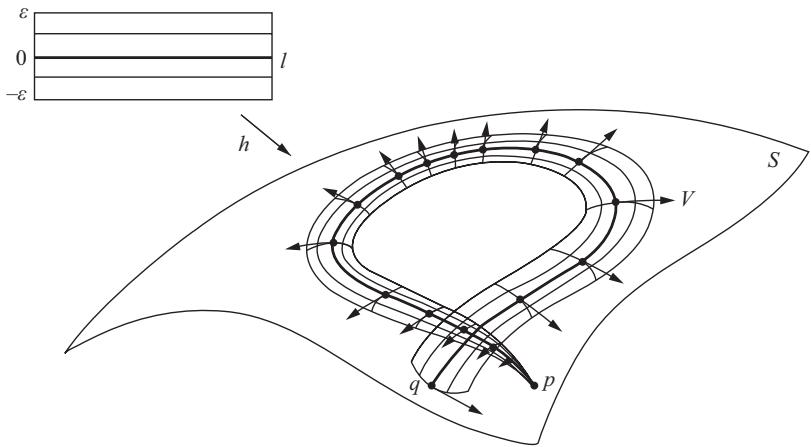
\includegraphics[width=\textwidth]{../../../PDFs/differential-geometry/transcript/Do Carmo - Differential Geometry of Curves and Surfaces/hybrid_ocr/images/3b2c5faa763a8cefdddf8608839bb7df8d3e556c44e581337b9e40ecc7d4c6c8.jpg}}
\end{minipage}
\end{figure}

\begin{figure}[H]
\centering
\begin{minipage}{0.55\textwidth}
\centering
\subfloat[Figure 5-14. (c) 小问中的几何构型]{\label{fig:fig5-14}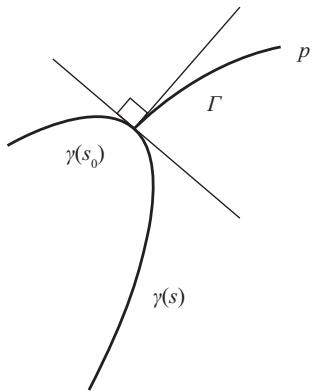
\includegraphics[width=\textwidth]{../../../PDFs/differential-geometry/transcript/Do Carmo - Differential Geometry of Curves and Surfaces/hybrid_ocr/images/b0507eebec0f2e639ed7f70f73f1aeae139ba72e68df67292ad2984512a50206.jpg}}
\end{minipage}
\end{figure}

\subsection*{5-4 节练习}

\begin{exercise}{5-4, 1 — do Carmo, Exercise 5-4, 1}
Bonnet 定理的逆命题是否成立？即：若 $S$ 紧致且直径 $\rho \leq \pi/\sqrt{\delta}$，是否必有 $K \geq \delta$？
\end{exercise}
\begin{solution}
\textbf{直观理解}: Bonnet 定理断言：$K \geq \delta > 0$ $\Rightarrow$ $\rho \leq \pi/\sqrt{\delta}$。其逆命题问的是：紧致直径有界 $\Rightarrow$ 曲率下界？直觉上，直径有界只限制了曲面"大小"，但不限制"弯曲程度"——可以在局部做剧烈弯曲而不改变直径。

\textbf{解答}: 逆命题不成立。考虑一个细长的环面（torus），其小圆方向有较大正曲率，而大圆方向曲率较小。调整环面的形状可以使直径满足 $\rho \leq \pi$（例如取半径接近的环面），但 $K$ 在某些点处可接近 $0$，不满足 $K \geq \delta > 0$。更简单的反例：取球冠（去掉部分 cap 的球面）的等距像，使其在赤道处稍加平坦化（保持紧致性），直径仍 $\leq \pi$，但 $K$ 在平坦化区域降低至接近 $0$。实际上，Bonnet 估计是最优的，但方向不可逆。\qed
\end{solution}

\begin{exercise}{5-4, 2* — Kazdan-Warner Remark, do Carmo, Exercise 5-4, 2}
设 $S = \{z=f(x,y); (x,y)\in\mathbb{R}^2\}$ 是完备非紧正则曲面。证明
\[
\lim_{r\to\infty}\left(\inf_{x^2+y^2\geq r}K(x,y)\right) \leq 0.
\]
\end{exercise}
\begin{solution}
\textbf{直观理解}: 完备非紧曲面在无穷远处必有"平坦化"的趋势。若 $K$ 在无穷远处有正下界，则由 Bonnet 定理的推广，曲面会紧致——与非紧矛盾。

\textbf{解答}: 设 $S = \{z = f(x,y)\}$ 是完备非紧正则曲面。假设结论不成立，即 $\liminf_{r\to\infty} K > 0$（存在 $\delta > 0$ 使在无穷远处 $K \geq \delta$）。取单位向量 $v = (0,0,1)$（$z$ 轴方向），高度函数 $h(x,y,z) = z = f(x,y)$。由第 5-3 节练习 10，$|\mathrm{grad}\,h| \leq 1$，且 $\mathrm{grad}\,h$ 的轨迹 $\alpha(t)$ 定义于整个 $\mathbb{R}$ 上。但更关键的是利用 Bonnet 定理的直径估计在无穷远处的应用。

考虑在无穷远处取点 $p_r = (r\cos\theta, r\sin\theta, f(r\cos\theta, r\sin\theta))$。由假设，$K(p_r) \geq \delta$。取 $q = (0,0,f(0,0))$ 为原点投影。对任意 $p_r$，设 $\gamma_r$ 是连接 $q$ 与 $p_r$ 的最小测地线。由第二变分公式（见第 5-4 节），若 $l(\gamma_r) > \pi/\sqrt{\delta}$，则存在变分使长度减少，与极小性矛盾。故对所有 $r$，有 $d(q,p_r) \leq \pi/\sqrt{\delta}$，即 $S$ 在内蕴距离下有界。由第 5-3 节推论 2，$S$ 紧致，与非紧假设矛盾。故 $\liminf_{r\to\infty} K \leq 0$。\footnote{另一种更直接的证明利用 Bonnet 定理的推广形式（Calabi-Schneider）和高度函数的梯度估计。}\qed
\end{solution}

\begin{exercise}{5-4, 3 — do Carmo, Exercise 5-4, 3}
（a）推导不假设变分是真变分时的第一变分公式。（b）设 $S$ 完备，$\gamma(s)$，$s\in\mathbb{R}$ 是 $S$ 上的测地线，$d(s) = d(\gamma(s),p)$ 是到固定点 $p$ 的距离。证明存在点 $s_0$ 使 $d(s_0) \leq d(s)$ 对所有 $s$ 成立，且连接 $p$ 与 $\gamma(s_0)$ 的测地线垂直于 $\gamma$（见 \cref{fig:fig5-14}）。（c）进一步假设 $S$ 与平面同胚且 $K \leq 0$，证明上述 $s_0$（从而上述垂线）是唯一的。
\end{exercise}

\begin{exercise}{5-4, 4*（变分学）— do Carmo, Exercise 5-4, 4}
设 $y=y(x)$，$x\in[x_1,x_2]$ 是平面曲线，变分 $y(x,t)$ 满足 $y(x,0)=y(x)$，$y(x_1,t)=y(x_1)$，$y(x_2,t)=y(x_2)$。考虑积分 $I(t) = \int_{x_1}^{x_2}F(x,y(x,t),y'(x,t))\,dx$。（a）证明：若 $y(x)$ 是 $I(t)$ 的临界点（$dI/dt=0$），则 $\int_{x_1}^{x_2}\eta(F_y - \frac{d}{dx}F_{y'})\,dx = 0$ 对所有满足 $\eta(x_1)=\eta(x_2)=0$ 的 $\eta$ 成立（变分法基本引理）。（b）推出 Euler-Lagrange 方程 $F_y - \frac{d}{dx}F_{y'} = 0$。（c）若 $F$ 不显含 $x$（即 $F=F(y,y')$），证明首次积分 $y'F_{y'} - F = \mathrm{const}$。
\end{exercise}

\begin{exercise}{5-4, 5*（变分学应用）— do Carmo, Exercise 5-4, 5}
（a）（最小面积旋转面。）设 $S$ 是由曲线 $y=f(x)$，$x\in[x_1,x_2]$ 绕 $x$ 轴旋转得到的旋转面。证明：若 $S$ 在所有生成旋转面中面积最小，则 $y = \frac{1}{c}\cosh(cx+c_1)$（悬链面）。（b）（旋转面的测地线。）设 $\mathbf{x}(u,v) = (f(v)\cos u, f(v)\sin u, g(v))$。证明测地线（除子午线和平行线外）满足 Clairaut 关系。\footnote{ Clairaut 公式原文为 $u' = c/(f^2)\sqrt{(f'^2+g'^2)(f^2-c^2)}^{-1}\cdot\sqrt{\cdots}$，此处有省略。}
\end{exercise}

% ==================== Section 5-5: Jacobi Fields and Conjugate Points ====================
\section{Jacobi Fields and Conjugate Points}\label{sec:jacobi-conjugate}

\textbf{Jacobi 场的动机.} 我们想研究给定测地线 $\gamma$ 附近测地线的行为。自然的做法是考虑那些本身也是测地线的变分——其变分场揭示了测地线在"并行"条件下的行为。

\begin{Definition}[Jacobi 场]\label{def:jacobi-field}
设 $\gamma: [0,l] \to S$ 是参数化测地线。称可微映射 $h: [0,l]\times(-\epsilon,\epsilon) \to S$ 是 $\gamma$ 的变分，如果对每个 $t$，曲线 $h_t(s) = h(s,t)$ 也是参数化测地线。变分场 $J(s) = (\partial h/\partial t)(s,0)$ 称为沿 $\gamma$ 的\textbf{Jacobi 场}（Jacobi field）。
\end{Definition}

\textbf{Trivial 例子.} 切向量场 $\gamma'(s)$ 本身是 Jacobi 场（取 $h(s,t) = \gamma(s+t)$）。

\begin{Proposition}\label{prop:jacobi-equation}
沿 $\gamma$ 的 Jacobi 场 $J(s)$ 满足 Jacobi 方程：
\[
\frac{D}{ds}\frac{D}{ds}J(s) + K(s)(\gamma'(s)\wedge J(s))\wedge\gamma'(s) = 0,
\]
其中 $K(s)$ 是 $S$ 在 $\gamma(s)$ 处的高斯曲率。
\end{Proposition}

\begin{Proof}
由 $h_t(s)$ 是测地线得 $(D/\partial s)(\partial h/\partial s) = 0$。对 $t$ 求偏导并用引理 \ref{curvature-commutation}（第 5-4 节）得
\[
0 = \frac{D}{\partial t}\frac{D}{\partial s}\frac{\partial h}{\partial s} = \frac{D}{\partial s}\frac{D}{\partial t}\frac{\partial h}{\partial s} + K\frac{\partial h}{\partial s}\wedge\frac{\partial h}{\partial t}\wedge\frac{\partial h}{\partial s}.
\]
在 $t=0$ 处取值得 Jacobi 方程。\footnote{详细推导见附录 \cref{sec:derivation-jacobi-equation}}
\end{Proof}

\begin{Remark}
Jacobi 方程是线性二阶常微分方程组，其解空间是 4 维向量空间。
\end{Remark}

\textbf{Example（球面上的 Jacobi 场）.} 单位球面 $S^2$ 的平行 $\theta=\pi/2$ 上的大圆弧 $\gamma(s)$（$s=\varphi-\varphi_0$，$0\leq s\leq\pi$）。沿 $\gamma$ 的平行运输单位正交向量场 $w(s)$，则
\[
J(s) = (\sin s)\,w(s)
\]
是 Jacobi 场（直接代入验证：$K=1$，$D^2J/ds^2 + KJ = -\sin s + \sin s = 0$）。注意 $J(0)=J(\pi)=0$。

\begin{Definition}[共轭点]\label{def:conjugate-point}
设 $\gamma: [0,l] \to S$，$\gamma(0)=p$。称点 $q=\gamma(s_0)$ 与 $p$ 关于 $\gamma$ \textbf{共轭}（conjugate），如果存在非零 Jacobi 场 $J(s)$ 沿 $\gamma$ 满足 $J(0)=J(s_0)=0$。
\end{Definition}

\textbf{直观含义.} 共轭点是"无限接近的"测地线的交点。球面上，任意一条从 $p$ 出发的测地线，其对径点就是与 $p$ 共轭的点（见 \cref{fig:fig5-18}）。

\begin{figure}[H]
\centering
\begin{minipage}{0.55\textwidth}
\centering
\subfloat[Figure 5-18. 球面上的 Jacobi 场：$J(s)=\sin s\,w(s)$，$J(\pi)=0$]{\label{fig:fig5-18}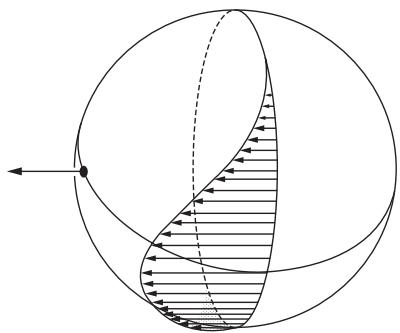
\includegraphics[width=\textwidth]{../../../PDFs/differential-geometry/transcript/Do Carmo - Differential Geometry of Curves and Surfaces/hybrid_ocr/images/8d4591e058e498f71e52247b45c12013977e762221b67942888a89ca8a539020.jpg}}
\end{minipage}
\end{figure}

\textbf{共轭点与指数映射的关系.} 设 $v = l\gamma'(0) \in T_p(S)$。则 $q = \exp_p(v)$ 与 $p$ 共轭，当且仅当 $v$ 是 $\exp_p: T_p(S) \to S$ 的临界点（命题 5）。这是共轭点的分析本质。

\begin{Proposition}\label{prop:conjugate-critical-point}
设 $p,q \in S$，$\gamma: [0,l] \to S$ 是连接 $p=\gamma(0)$ 与 $q=\exp_p(l\gamma'(0))$ 的测地线。则 $q$ 与 $p$ 关于 $\gamma$ 共轭，当且仅当 $v = l\gamma'(0)$ 是 $\exp_p$ 的临界点。
\end{Proposition}

\begin{Theorem}\label{no-conjugate-negative-curvature}
设曲面 $S$ 的高斯曲率 $K \leq 0$。则对任意 $p \in S$，$p$ 的共轭轨迹为空——即 $K \leq 0$ 的曲面没有共轭点。
\end{Theorem}

\begin{Proof}
设存在非平凡 Jacobi 场 $J(s)$ 沿 $\gamma$ 满足 $J(0)=J(l)=0$。由第 5-5 节的性质，$\langle J(s),\gamma'(s)\rangle = 0$。从 Jacobi 方程和 $K \leq 0$ 可得
\[
\frac{d}{ds}\left\langle \frac{DJ}{ds}, J\right\rangle = \left|\frac{DJ}{ds}\right|^2 - K|J|^2 \geq 0.
\]
由于 $\langle DJ/ds,J\rangle$ 在 $s=0$ 和 $s=l$ 处均为零（因为 $J(0)=J(l)=0$），上式说明 $\langle DJ/ds,J\rangle \equiv 0$，从而 $|J|^2 = \mathrm{const}$。由 $J(0)=0$ 得 $J\equiv 0$，矛盾。\footnote{详细推导见附录 \cref{sec:derivation-no-conjugate}}
\end{Proof}

\textbf{推论.} 若 $K \leq 0$，则 $\exp_p: T_p(S) \to S$ 是局部微分同胚（由逆函数定理）。

\textbf{Example.} 平面（$K=0$）和旋转双曲面（$K<0$）都没有共轭点。柱面（$K=0$）的测地线（圆、螺旋线、直线）也没有共轭点。

\begin{Lemma}[Gauss]\label{gauss-lemma}
设 $p \in S$，$\mathbf{u} \in T_p(S)$，$\mathbf{w} \in (T_p(S))_\mathbf{u}$。则
\[
\langle \mathbf{u}, \mathbf{w}\rangle = \langle (d\exp_p)_\mathbf{u}(\mathbf{u}), (d\exp_p)_\mathbf{u}(\mathbf{w})\rangle.
\]
\end{Lemma}

\textbf{几何意义.} 该引理说明在法坐标系中，测地线是"径向"的，且径向测地线与测地圆正交（这推广了法坐标系中测地圆正交于径向测地线的性质）。

\begin{Remark}
共轭点的存在性与曲率分布密切相关：正曲率使测地线最终会聚（球面共轭），负曲率使测地线发散（无共轭点）。这是 Jacobi 场理论的核心几何现象。
\end{Remark}

\begin{Remark}
一般椭球面的共轭轨迹（conjugate locus）是一条曲线（见 \cref{fig:fig5-19}）。球面是唯一所有共轭轨迹都缩约成单点的曲面（这是 L. Green 的一个深刻结果）。
\end{Remark}

\begin{figure}[H]
\centering
\begin{minipage}{0.55\textwidth}
\centering
\subfloat[Figure 5-19. 椭球面的共轭轨迹]{\label{fig:fig5-19}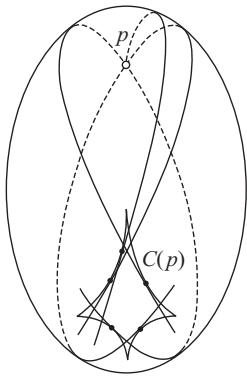
\includegraphics[width=\textwidth]{../../../PDFs/differential-geometry/transcript/Do Carmo - Differential Geometry of Curves and Surfaces/hybrid_ocr/images/00ba2e82b8c9203c068529df1f226052e698011e2f85a9c9e7fd9bd7fe241554.jpg}}
\end{minipage}
\end{figure}

\begin{figure}[H]
\centering
\begin{minipage}{0.55\textwidth}
\centering
\subfloat[Figure 5-16. 指数映射的微分几何意义]{\label{fig:fig5-16}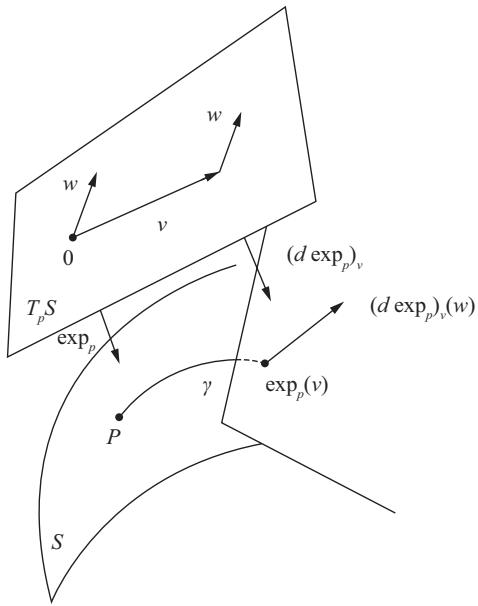
\includegraphics[width=\textwidth]{../../../PDFs/differential-geometry/transcript/Do Carmo - Differential Geometry of Curves and Surfaces/hybrid_ocr/images/0c5380d22284c20ad43fd260afcbe6dbe28a06d22eb7ccc98dea17d690a3c559.jpg}}
\end{minipage}
\end{figure}

\begin{figure}[H]
\centering
\begin{minipage}{0.55\textwidth}
\centering
\subfloat[Figure 5-17. Jacobi 场的构造：$J(s)=s(d\exp_p)_{sv}(w)$]{\label{fig:fig5-17}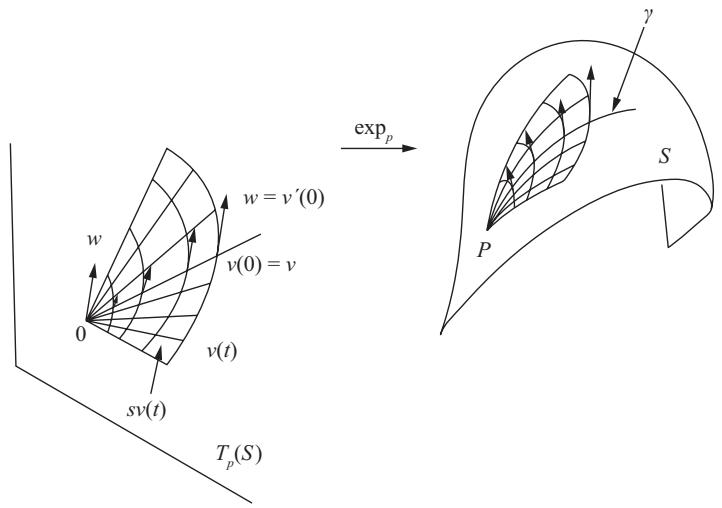
\includegraphics[width=\textwidth]{../../../PDFs/differential-geometry/transcript/Do Carmo - Differential Geometry of Curves and Surfaces/hybrid_ocr/images/ccf3838c806db8e32228ed9891f30b1014df2cdb711c624e29773e4ae6a5c1a8.jpg}}
\end{minipage}
\end{figure}

\begin{figure}[H]
\centering
\begin{minipage}{0.55\textwidth}
\centering
\subfloat[Figure 5-20. Gauss 引理的证明构造]{\label{fig:fig5-20}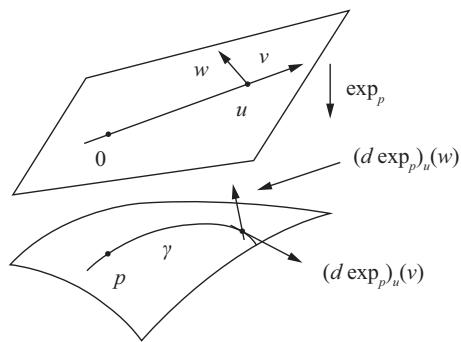
\includegraphics[width=\textwidth]{../../../PDFs/differential-geometry/transcript/Do Carmo - Differential Geometry of Curves and Surfaces/hybrid_ocr/images/1ba2e22f1f13d88ddd6d0d38ec454df7a18ff5cc9e35a976744294b3a9f20577.jpg}}
\end{minipage}
\end{figure}

\begin{Remark}
第 5-5 节建立的 Jacobi 场理论，将在第 5-6 节（覆叠空间）和第 5-8 节（零曲率曲面）中发挥关键作用。
\end{Remark}

\subsection*{5-5 节练习}

\begin{exercise}{5-5, 1 — do Carmo, Exercise 5-5, 1}
（a）设 $\gamma: [0,l] \to S$ 是弧长参数测地线，$J(s)$ 是沿 $\gamma$ 的 Jacobi 场满足 $J(0)=0$，$\langle J'(0),\gamma'(0)\rangle = 0$。证明 $\langle J(s),\gamma'(s)\rangle = 0$ 对所有 $s$ 成立。（b）进一步设 $|J'(0)|=1$，取 $\{e_1(s),e_2(s)\}$ 为沿 $\gamma$ 的平行正交基，$e_1(0)=\gamma'(0)$，$e_2(0)=J'(0)$。证明 $J(s)=u(s)e_2(s)$，其中 $u(s)$ 满足 $u''+K(s)u=0$，$u(0)=0$，$u'(0)=1$。
\end{exercise}

\begin{exercise}{5-5, 2 — do Carmo, Exercise 5-5, 2}
证明：抛物面 $z=x^2+y^2$ 上从原点 $p=(0,0,0)$ 出发的任意测地线均无共轭点。
\end{exercise}

\begin{exercise}{5-5, 3*（比较定理）— do Carmo, Exercise 5-5, 3}
设 $S$ 和 $\tilde{S}$ 是完备曲面，$p\in S$，$\tilde{p}\in\tilde{S}$，$i: T_p(S) \to T_{\tilde{p}}(\tilde{S})$ 是线性等距。设 $\gamma: [0,\infty) \to S$ 是测地线，$J(s)$ 是沿 $\gamma$ 的 Jacobi 场满足 $J(0)=0$，$\langle J'(0),\gamma'(0)\rangle=0$，$|J'(0)|=1$。（a）证明：$J(s)=v(s)e_2(s)$，$\tilde{J}(s)=u(s)\tilde{e}_2(s)$，其中 $v$ 和 $u$ 分别满足 $v''+K(s)v=0$，$v(0)=0$，$v'(0)=1$ 和 $u''+\tilde{K}(s)u=0$，$u(0)=0$，$u'(0)=1$。（b）（第一比较定理）假设 $K(s)\leq \tilde{K}(s)$，$s\in[0,\infty)$，证明：若 $\tilde{\gamma}$ 的首个共轭点出现在 $s=a$，则 $\gamma$ 的首个共轭点不早于 $s=a$。（c）（第二比较定理）在同样假设下，证明 $|J(s)| \geq |\tilde{J}(s)|$ 对所有 $s\in[0,a)$ 成立。（d）证明：在 (c) 中，等号恒成立当且仅当 $K(s)=\tilde{K}(s)$。
\end{exercise}

\begin{exercise}{5-5, 4 — do Carmo, Exercise 5-5, 4}
设 $S$ 是高斯曲率 $K \leq K_0$（$K_0>0$ 常数）的完备曲面。利用第一比较定理，证明：任意测地线 $\gamma: [0,\infty) \to S$ 在区间 $(0,\pi/\sqrt{K_0}]$ 内无共轭点。
\end{exercise}

\begin{exercise}{5-5, 5 — do Carmo, Exercise 5-5, 5}
设 $S$ 是高斯曲率 $K \geq K_1 > 0$ 的完备曲面。证明：任意测地线 $\gamma: [0,\infty) \to S$ 在区间 $(0,\pi/\sqrt{K_1}]$ 内必有共轭点。
\end{exercise}

\begin{exercise}{5-5, 6*（Sturm 振荡定理）— do Carmo, Exercise 5-5, 6}
设 $S$ 完备，$\gamma: [0,\infty) \to S$ 是测地线，$J(s)$ 是沿 $\gamma$ 的 Jacobi 场满足 $J(0)=J(s_0)=0$，$s_0\in(0,\infty)$，且 $J(s)\neq 0$ 对 $s\in(0,s_0)$。设 $K(s)\leq L(s)$，其中 $L$ 是 $[0,\infty)$ 上的可微函数。证明：微分方程 $u''+L(s)u=0$ 的每个解在区间 $(0,s_0]$ 上必有零点。
\end{exercise}

\begin{exercise}{5-5, 7*（Kneser 共轭点判据）— do Carmo, Exercise 5-5, 7}
设 $\gamma: [0,\infty) \to S$ 是完备曲面 $S$ 上的测地线，$\gamma(0)=p$，$K(s)$ 是沿 $\gamma$ 的高斯曲率。假设 $\int_t^\infty K(s)\,ds \leq \frac{1}{4(t+1)}$ 对所有 $t\geq 0$ 成立（积分收敛且有界）。（a）定义 $w(t) = \int_t^\infty K(s)\,ds + \frac{1}{4(t+1)}$，证明 $w'(t)+w(t)^2 \leq -K(t)$。（b）设 $w'(t)+w(t)^2 = -L(t)$（故 $L(t)\geq K(t)$），定义 $v(t) = \exp(\int_0^t w(s)\,ds)$。证明 $v''(t)+L(t)v(t)=0$，$v(0)=1$，$v'(0)=0$。（c）由 Sturm 振荡定理证明：若上述不等式成立，则 $\gamma$ 上无点与 $p$ 共轭。
\end{exercise}

\begin{exercise}{5-5, 8* — do Carmo, Exercise 5-5, 8}
设 $\gamma: [0,l] \to S$ 是完备曲面 $S$ 上的测地线，$\gamma(l)$ 与 $\gamma(0)$ 不共轭。设 $w_0 \in T_{\gamma(0)}(S)$，$w_1 \in T_{\gamma(l)}(S)$。证明：存在唯一的沿 $\gamma$ 的 Jacobi 场 $J(s)$ 满足 $J(0)=w_0$，$J(l)=w_1$。
\end{exercise}

\begin{exercise}{5-5, 9 — do Carmo, Exercise 5-5, 9}
设 $J(s)$ 是沿测地线 $\gamma: [0,l] \to S$ 的 Jacobi 场，满足 $\langle J(0),\gamma'(0)\rangle = 0$ 且 $J'(0)=0$。证明 $\langle J(s),\gamma'(s)\rangle = 0$ 对所有 $s$ 成立。
\end{exercise}

% ==================== Section 5-6: Covering Spaces; The Theorems of Hadamard ====================
\section{Covering Spaces; The Theorems of Hadamard}\label{sec:hadamard}

上一节已证明：若 $K \leq 0$，则 $\exp_p: T_p(S) \to S$ 是局部微分同胚。本节追问：何时局部微分同胚是整体微分同胚？这引出了覆叠空间的理论。

% A. 覆叠空间
\subsection*{A. 覆叠空间}

\begin{Definition}[覆叠映射]\label{def:covering-map}
设 $\tilde{B}, B \subset \mathbb{R}^3$。映射 $\pi: \tilde{B} \to B$ 称为\textbf{覆叠映射}（covering map），如果：
\begin{enumerate}
  \item $\pi$ 连续且 $\pi(\tilde{B}) = B$；
  \item 每点 $p \in B$ 都有邻域 $U$（称为\textbf{基域}，distinguished neighborhood），使得 $\pi^{-1}(U) = \bigcup_\alpha V_\alpha$，其中各 $V_\alpha$ 互不相交，且 $\pi|_{V_\alpha}: V_\alpha \to U$ 是同胚。
\end{enumerate}
此时 $\tilde{B}$ 称为 $B$ 的\textbf{覆叠空间}（covering space）。
\end{Definition}

\textbf{Example 1（平面覆叠柱面）.} 平面 $P$ 通过 $\pi(u,v) = (\cos u, \sin u, v)$ 覆叠圆柱面 $S = \{(x,y,z): x^2+y^2=1\}$（见 \cref{fig:fig5-22}）。直观上：将平面"卷"向圆柱面，无穷多层。

\begin{figure}[H]
\centering
\begin{minipage}{0.55\textwidth}
\centering
\subfloat[Figure 5-22. 平面覆叠圆柱面：将平面卷向圆柱面]{\label{fig:fig5-22}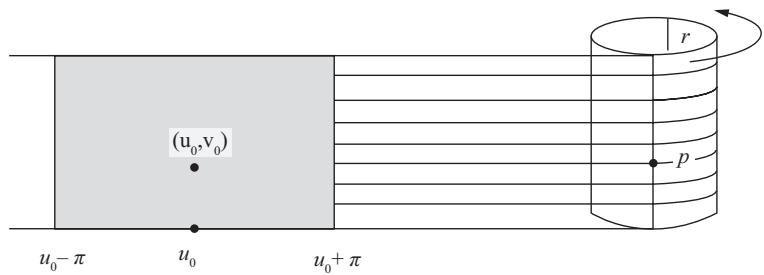
\includegraphics[width=\textwidth]{../../../PDFs/differential-geometry/transcript/Do Carmo - Differential Geometry of Curves and Surfaces/hybrid_ocr/images/e3bfbd94692ad63e4461772c4d8ced89c2c53cbca64ab6e61c47a13e7b67383f.jpg}}
\end{minipage}
\end{figure}

\textbf{Example 2（螺旋线覆叠圆）.} 螺旋线 $H = \{(\cos t, \sin t, bt): t\in\mathbb{R}\}$ 通过 $\pi(x,y,z) = (x,y,0)$ 覆叠单位圆 $S^1$（见 \cref{fig:fig5-23}）。

\begin{figure}[H]
\centering
\begin{minipage}{0.55\textwidth}
\centering
\subfloat[Figure 5-23. 螺旋线覆叠圆]{\label{fig:fig5-23}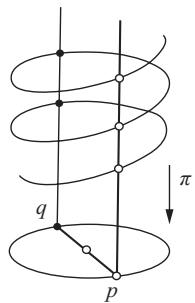
\includegraphics[width=\textwidth]{../../../PDFs/differential-geometry/transcript/Do Carmo - Differential Geometry of Curves and Surfaces/hybrid_ocr/images/ac958466d6b11de3d23faca24b2240c942baf95a7a3335bc0919820123ad15cb.jpg}}
\end{minipage}
\end{figure}

\textbf{Example 4（圆覆叠圆）.} $k$ 次覆叠映射 $\pi(\cos t, \sin t) = (\cos kt, \sin kt)$ 是 $k$ 叶覆叠。

\textbf{覆叠空间的提升性质.} 覆叠空间的核心性质是任何曲线都可以"提升"到覆叠空间中。

\begin{Proposition}\label{prop:lifting-arcs}
设 $\pi: \tilde{B} \to B$ 是覆叠映射，$\alpha: [0,l] \to B$ 是 $B$ 中弧线，$\tilde{p}_0 \in \tilde{B}$ 满足 $\pi(\tilde{p}_0) = \alpha(0)$。则存在唯一的提升 $\tilde{\alpha}: [0,l] \to \tilde{B}$ 使 $\tilde{\alpha}(0) = \tilde{p}_0$ 且 $\pi\circ\tilde{\alpha} = \alpha$。
\end{Proposition}

\begin{Definition}[单连通]\label{def:simply-connected}
弧道连通的集合 $B \subset \mathbb{R}^3$ 称为\textbf{单连通的}（simply connected），如果任意两条端点相同的弧线均同伦。特别地，任意闭弧线（起点终点相同）均与常值弧线同伦。
\end{Definition}

直观上：单连通 = "没有洞"；任意闭曲线可以连续收缩为一点。平面和球面是单连通的；环面和圆柱面不是。

\textbf{关键结果.}

\begin{Proposition}\label{prop:covering-homeomorphism}
设 $\pi: \tilde{B} \to B$ 是局部同胚（且有提升弧线的性质），$\tilde{B}$ 弧道连通，$B$ 单连通。则 $\pi$ 是同胚。
\end{Proposition}

\begin{Proof}[证明概要]
只需证明 $\pi$ 是单射。设 $\tilde{p}_1, \tilde{p}_2 \in \tilde{B}$，$\pi(\tilde{p}_1)=\pi(\tilde{p}_2)=p$。取 $\tilde{B}$ 中连接 $\tilde{p}_1$ 与 $\tilde{p}_2$ 的弧 $\tilde{\alpha}_0$，其投影 $\alpha_0 = \pi\circ\tilde{\alpha}_0$ 是 $B$ 中闭弧线。因 $B$ 单连通，$\alpha_0$ 与常值弧线同伦。提升同伦得 $\tilde{\alpha}_0$ 与常值弧线同伦，从而 $\tilde{p}_1=\tilde{p}_2$。\footnote{详细推导见附录 \cref{sec:derivation-covering-homeomorphism}}
\end{Proof}

% B. Hadamard 定理
\subsection*{B. Hadamard 定理}

现在回到本节的核心问题：何时 $\exp_p: T_p(S) \to S$ 是整体微分同胚？

\begin{Lemma}\label{length-increasing}
设 $S$ 是高斯曲率 $K \leq 0$ 的完备曲面。则 $\exp_p: T_p(S) \to S$ 是长度增的：即对任意 $\mathbf{u}, \mathbf{w} \in T_p(S)$，
\[
\langle (d\exp_p)_\mathbf{u}(\mathbf{w}), (d\exp_p)_\mathbf{u}(\mathbf{w})\rangle \geq \langle \mathbf{w}, \mathbf{w}\rangle.
\]
\end{Lemma}

\begin{Proof}[证明概要]
归结为 $K \leq 0$ 时 Jacobi 场的性质。利用引理 \ref{gauss-lemma}（Gauss）和 Jacobi 方程，可证 $|J(s)|^2 \geq s^2|w|^2$，取 $s=|u|$ 即得所需不等式。\footnote{详细推导见附录 \cref{sec:derivation-length-increasing}}
\end{Proof}

\begin{Corollary}
若 $K \equiv 0$，则 $\exp_p: T_p(S) \to S$ 是局部等距。
\end{Corollary}

\begin{Proposition}\label{prop:exp-covering-map}
设 $S$ 是高斯曲率 $K \leq 0$ 的完备曲面。则 $\exp_p: T_p(S) \to S$ 是覆叠映射。
\end{Proposition}

\begin{Proof}
已知 $\exp_p$ 是局部微分同胚，只需证明它有提升弧线的性质。利用弧长增性，可以控制弧线的提升——若提升不完整则导致弧长无界的矛盾。\footnote{详细推导见附录 \cref{sec:derivation-exp-covering}}
\end{Proof}

\begin{Theorem}[Hadamard 第一定理]\label{hadamard-first}
设 $S$ 是单连通、完备曲面，高斯曲率 $K \leq 0$。则 $\exp_p: T_p(S) \to S$ 是微分同胚；即 $S$ 微分同胚于平面。
\end{Theorem}

\begin{Proof}
由命题 \ref{prop:exp-covering-map}，$\exp_p$ 是覆叠映射。$T_p(S)$ 与平面同构（作为向量空间）显然是单连通的。由命题 \ref{prop:covering-homeomorphism}，覆叠映射 $\exp_p: T_p(S) \to S$ 是同胚；它是局部微分同胚，故其逆也可微，从而是微分同胚。\qed
\end{Proof}

\begin{Theorem}[Hadamard 第二定理]\label{hadamard-second}
设 $S$ 是卵形面（紧致、连通、正高斯曲率的正则曲面）。则 Gauss 映射 $N: S \to S^2$ 是微分同胚；特别地，$S$ 微分同胚于球面。
\end{Theorem}

\begin{Proof}
$K>0$ 意味着 $N$ 是局部微分同胚（$dN_p$ 可逆）。由命题 \ref{prop:covering-homeomorphism}（紧致 $\Rightarrow$ 覆叠映射），$N$ 是覆叠映射。$S^2$ 单连通，故 $N$ 是同胚。局部微分同胚 + 同胚 $\Rightarrow$ 微分同胚。\footnote{详细推导见附录 \cref{sec:derivation-hadamard-second}}
\end{Proof}

\begin{Remark}
Hadamard 第二定理的几何意义更强：由于 Gauss 映射是微分同胚，每一单位向量恰好出现一次为 $S$ 的法向量，由此推出卵形面是局部凸的——它位于每一切平面的一侧。事实上，卵形面是某凸集（凸体）的边界。
\end{Remark}

\begin{Remark}
Hadamard 第一定理也可由 Klingenberg 引理（练习 8）给出更简洁的证明（见练习 9）。这体现了覆叠空间理论的强大威力。
\end{Remark}

\begin{figure}[H]
\centering
\begin{minipage}{0.55\textwidth}
\centering
\subfloat[Figure 5-24. 命题 1 证明中的构造：$\pi$ 是局部同胚，$U$ 是基域]{\label{fig:fig5-24}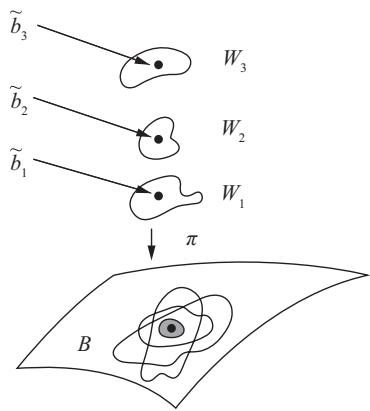
\includegraphics[width=\textwidth]{../../../PDFs/differential-geometry/transcript/Do Carmo - Differential Geometry of Curves and Surfaces/hybrid_ocr/images/72072d771829ae9baf4cddb32e550b6e240d3551a4cc633238d8000425ba2a7f.jpg}}
\end{minipage}
\end{figure}

\begin{Remark}
本节中的 Hadamard 定理是整体微分几何的里程碑结果：它们建立了曲率条件（$K \leq 0$ 或 $K>0$）与整体拓扑（平面型或球面型）之间的深刻联系。
\end{Remark}

\begin{Remark}
Hadamard 定理的更一般形式涉及完整曲面（complete surfaces）和更弱的曲率条件，这些在现代黎曼几何中有重要推广。
\end{Remark}

\begin{figure}[H]
\centering
\begin{minipage}{0.55\textwidth}
\centering
\subfloat[Figure 5-25. 弧线提升的构造：逐步在每个基域上延拓提升弧线]{\label{fig:fig5-25}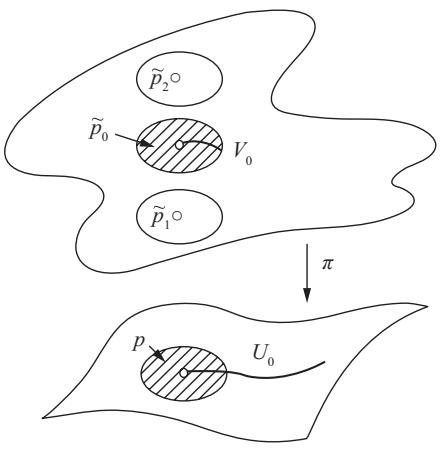
\includegraphics[width=\textwidth]{../../../PDFs/differential-geometry/transcript/Do Carmo - Differential Geometry of Curves and Surfaces/hybrid_ocr/images/df62e07203a43bf2814074f03ecdbcf2613cda45f278670c87e811bc44afdb74.jpg}}
\end{minipage}
\end{figure}

\begin{figure}[H]
\centering
\begin{minipage}{0.40\textwidth}
\centering
\subfloat[Figure 5-26. 单连通性的直观含义：任何闭弧线可缩到一点]{\label{fig:fig5-26a}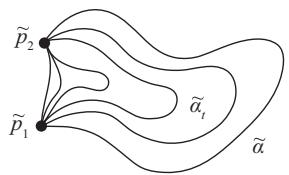
\includegraphics[width=\textwidth]{../../../PDFs/differential-geometry/transcript/Do Carmo - Differential Geometry of Curves and Surfaces/hybrid_ocr/images/550e844cd15958bac810049ea5e2c08452c4ae2a6a8f33ab430d23c89d4ef9bd.jpg}}
\end{minipage}
\hfill
\begin{minipage}{0.40\textwidth}
\centering
\subfloat[Figure 5-26b]{\label{fig:fig5-26b}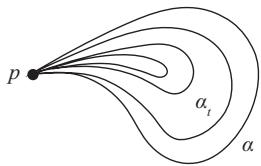
\includegraphics[width=\textwidth]{../../../PDFs/differential-geometry/transcript/Do Carmo - Differential Geometry of Curves and Surfaces/hybrid_ocr/images/7126bec9098d5dbbddda617859fc4e77db4b088104d7ba2726a4ccd7221a1714.jpg}}
\end{minipage}
\end{figure}

\begin{figure}[H]
\centering
\begin{minipage}{0.55\textwidth}
\centering
\subfloat[Figure 5-27. 同伦的概念：连续形变]{\label{fig:fig5-27}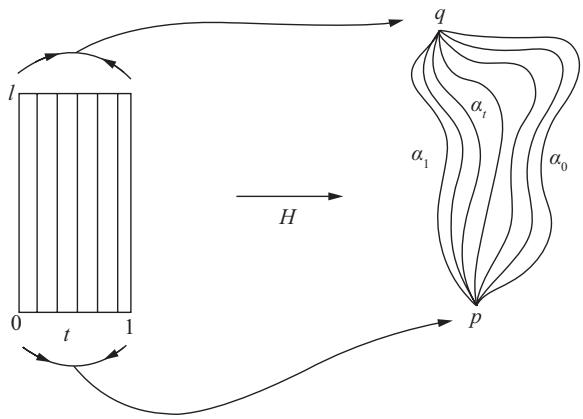
\includegraphics[width=\textwidth]{../../../PDFs/differential-geometry/transcript/Do Carmo - Differential Geometry of Curves and Surfaces/hybrid_ocr/images/2484e82cc1d0aca25cf6b5624d150b5db441be552864e152f42880a62d684bac.jpg}}
\end{minipage}
\end{figure}

\begin{figure}[H]
\centering
\begin{minipage}{0.55\textwidth}
\centering
\subfloat[Figure 5-28. 同伦的提升：$\tilde{H}$ 是 $H$ 的提升]{\label{fig:fig5-28}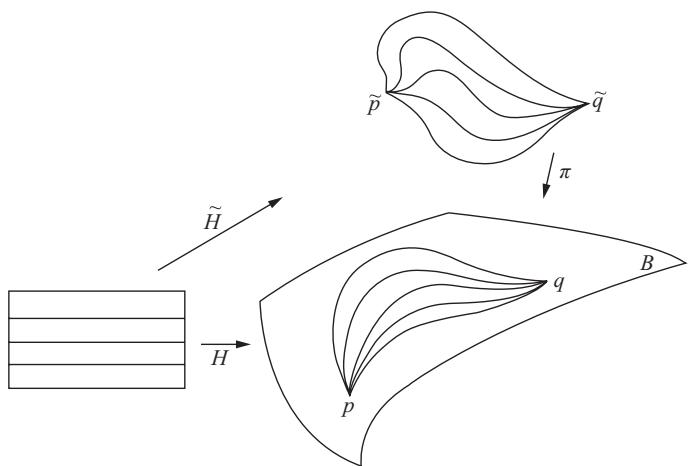
\includegraphics[width=\textwidth]{../../../PDFs/differential-geometry/transcript/Do Carmo - Differential Geometry of Curves and Surfaces/hybrid_ocr/images/305d4226ea89668d1cddd4225ec2e0479d106c7b39857a16dfc76613f6e53e7c.jpg}}
\end{minipage}
\end{figure}

\begin{figure}[H]
\centering
\begin{minipage}{0.55\textwidth}
\centering
\subfloat[Figure 5-29. Klingenberg 引理：同伦中的曲线长度约束]{\label{fig:fig5-29}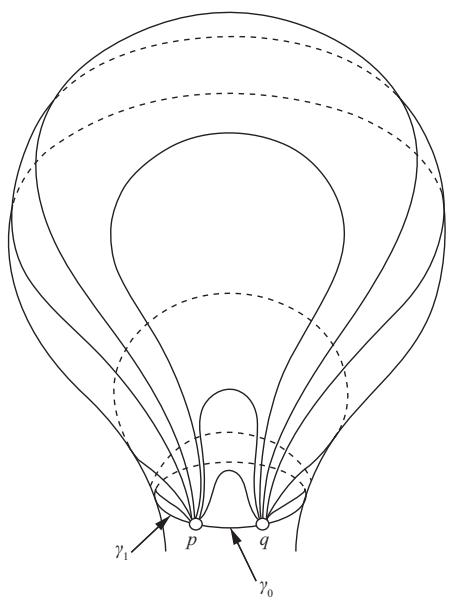
\includegraphics[width=\textwidth]{../../../PDFs/differential-geometry/transcript/Do Carmo - Differential Geometry of Curves and Surfaces/hybrid_ocr/images/a4e1cab17841331a906c758419c7a76a79a652f7da38e7b1cda3da2bec307976.jpg}}
\end{minipage}
\end{figure}

\begin{figure}[H]
\centering
\begin{minipage}{0.55\textwidth}
\centering
\subfloat[Figure 5-12. Osserman 引理构造：$\theta^{-1}$ 在 $\eta_0$ 处不能解析延拓]{\label{fig:fig5-12}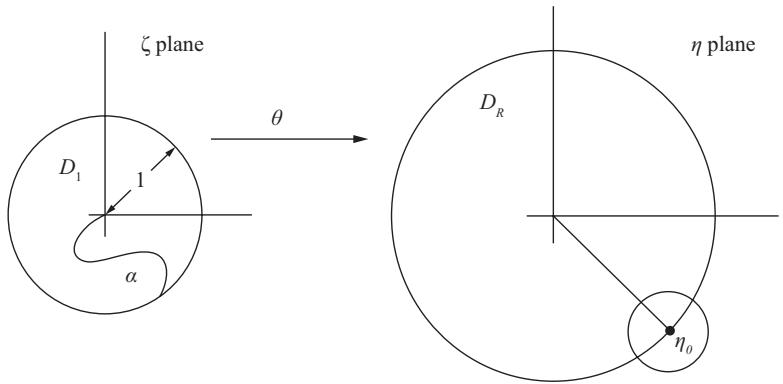
\includegraphics[width=\textwidth]{../../../PDFs/differential-geometry/transcript/Do Carmo - Differential Geometry of Curves and Surfaces/hybrid_ocr/images/37eccd0bc964efb812130f31b56fa0dccbf621e0e4807347e4b95a5f2f2d9955.jpg}}
\end{minipage}
\end{figure}

\begin{figure}[H]
\centering
\begin{minipage}{0.55\textwidth}
\centering
\subfloat[Figure 5-21. 比较定理的几何意义]{\label{fig:fig5-21}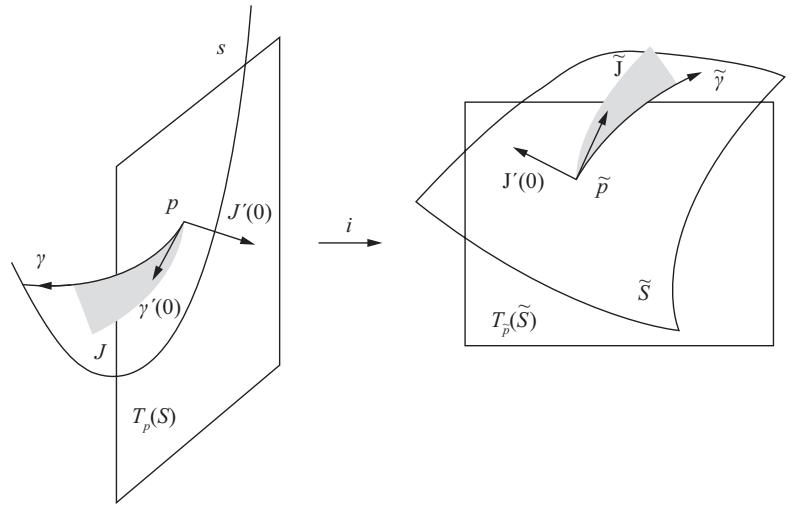
\includegraphics[width=\textwidth]{../../../PDFs/differential-geometry/transcript/Do Carmo - Differential Geometry of Curves and Surfaces/hybrid_ocr/images/2703746efbe014be8e70b18ae5de212974b11f0dc9bdb5f061d5c931cda00acb.jpg}}
\end{minipage}
\end{figure}

\begin{figure}[H]
\centering
\begin{minipage}{0.55\textwidth}
\centering
\subfloat[Figure 5-10. Hopf-Rinow 证明中的迭代构造]{\label{fig:fig5-10}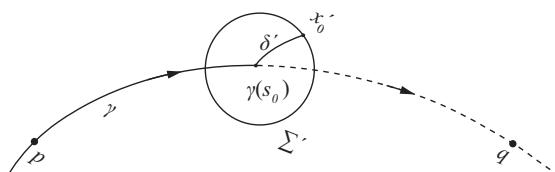
\includegraphics[width=\textwidth]{../../../PDFs/differential-geometry/transcript/Do Carmo - Differential Geometry of Curves and Surfaces/hybrid_ocr/images/32688213fa24fe9bf4d2f4b4602ad6f6db1b6979fd4a5374394c86cfbfc61096.jpg}}
\end{minipage}
\end{figure}

\begin{figure}[H]
\centering
\begin{minipage}{0.40\textwidth}
\centering
\subfloat[Figure 5-4. 可延展性证明：$p \in \mathrm{Bd}\,S$ 的邻域构造]{\label{fig:fig5-4}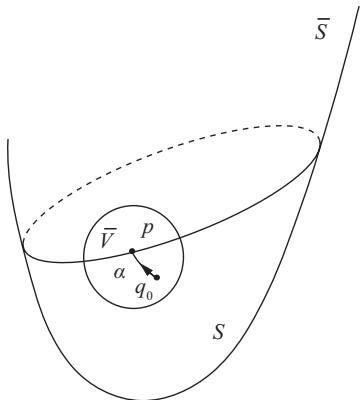
\includegraphics[width=\textwidth]{../../../PDFs/differential-geometry/transcript/Do Carmo - Differential Geometry of Curves and Surfaces/hybrid_ocr/images/c5ceac5048eb5b04b3b016f8f601975a97e4c9ad43209bec4ecf190ca1ad8f81.jpg}}
\end{minipage}
\end{figure}

\begin{figure}[H]
\centering
\begin{minipage}{0.40\textwidth}
\centering
\subfloat[Figure 5-8. $S^2-\{p\}$ 上两点之间无最小测地线的例子]{\label{fig:fig5-8}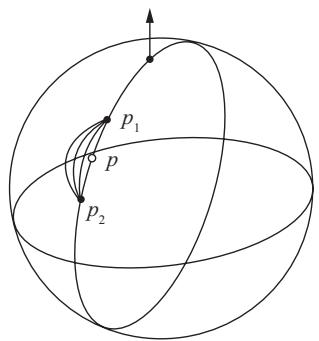
\includegraphics[width=\textwidth]{../../../PDFs/differential-geometry/transcript/Do Carmo - Differential Geometry of Curves and Surfaces/hybrid_ocr/images/e3577faf80b8116bbc28fadd9a8c1c691696a220096cd55933052dc58e30794d.jpg}}
\end{minipage}
\end{figure}

\begin{figure}[H]
\centering
\begin{minipage}{0.40\textwidth}
\centering
\subfloat[Figure 5-6. 锥面不可延展性的证明构造]{\label{fig:fig5-6}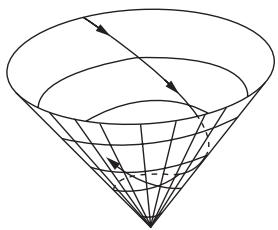
\includegraphics[width=\textwidth]{../../../PDFs/differential-geometry/transcript/Do Carmo - Differential Geometry of Curves and Surfaces/hybrid_ocr/images/25e37750a55f0a6edfb0076e4f81d3864b22bdbe9c906bae755249d931588687.jpg}}
\end{minipage}
\end{figure}

\begin{figure}[H]
\centering
\begin{minipage}{0.40\textwidth}
\centering
\subfloat[Figure 5-30. 度的概念：连续映射 $\varphi: S^1 \to S^1$ 的环绕数}{\label{fig:fig5-30}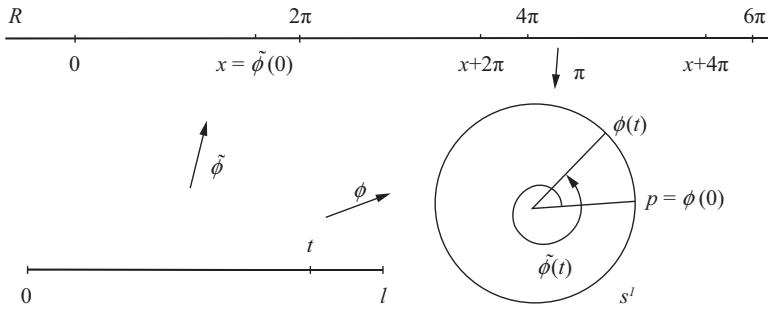
\includegraphics[width=\textwidth]{../../../PDFs/differential-geometry/transcript/Do Carmo - Differential Geometry of Curves and Surfaces/hybrid_ocr/images/6a2a83fbe7c561cc2c2612c4b21143a6ae2b340e445c7cef9c7178107d456bf4.jpg}}
\end{minipage}
\end{figure}

\begin{figure}[H]
\centering
\begin{minipage}{0.40\textwidth}
\centering
\subfloat[Figure 5-31. 旋转指标的几何含义]{\label{fig:fig5-31}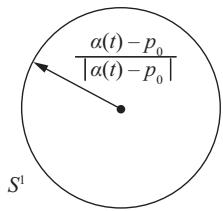
\includegraphics[width=\textwidth]{../../../PDFs/differential-geometry/transcript/Do Carmo - Differential Geometry of Curves and Surfaces/hybrid_ocr/images/d60712ab909c56ce528722f32b86f952b07bb46ddf5fe6153b5252a5d172a579.jpg}}
\end{minipage}
\end{figure}

\begin{figure}[H]
\centering
\begin{minipage}{0.40\textwidth}
\centering
\subfloat[Figure 5-31b]{\label{fig:fig5-31b}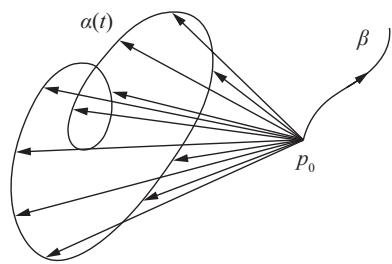
\includegraphics[width=\textwidth]{../../../PDFs/differential-geometry/transcript/Do Carmo - Differential Geometry of Curves and Surfaces/hybrid_ocr/images/532bd358dd4d393e2b4d298acf95b6813ebf647bac21ee32526db7ba750b2e3c.jpg}}
\end{minipage}
\end{figure}

\begin{figure}[H]
\centering
\begin{minipage}{0.40\textwidth}
\centering
\subfloat[Figure 5-32. Jordan 曲线定理的证明构造]{\label{fig:fig5-32}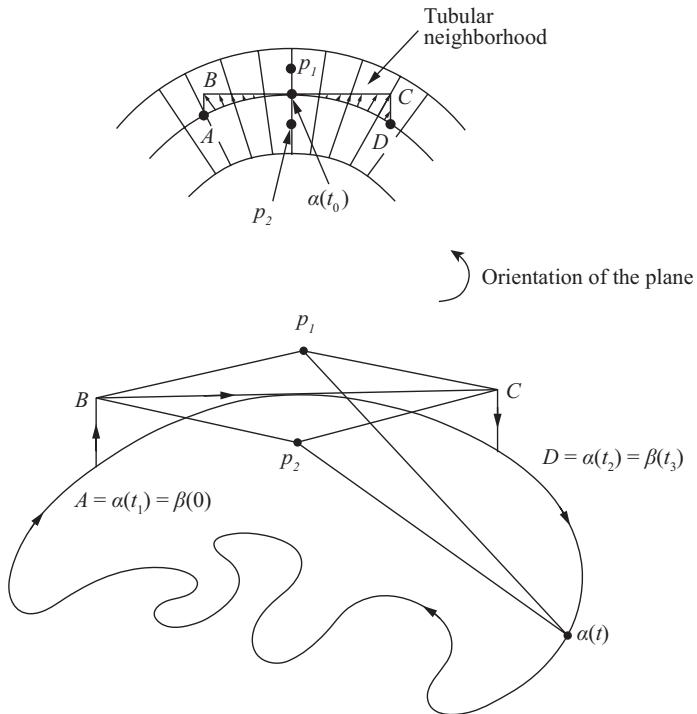
\includegraphics[width=\textwidth]{../../../PDFs/differential-geometry/transcript/Do Carmo - Differential Geometry of Curves and Surfaces/hybrid_ocr/images/ac899bd67abfac260b038cef1d192d46d911ba7779ed1ea885d74c933d990bcd.jpg}}
\end{minipage}
\end{figure}

\begin{figure}[H]
\centering
\begin{minipage}{0.40\textwidth}
\centering
\subfloat[Figure 5-33. 旋转定理的证明：割线映射]{\label{fig:fig5-33}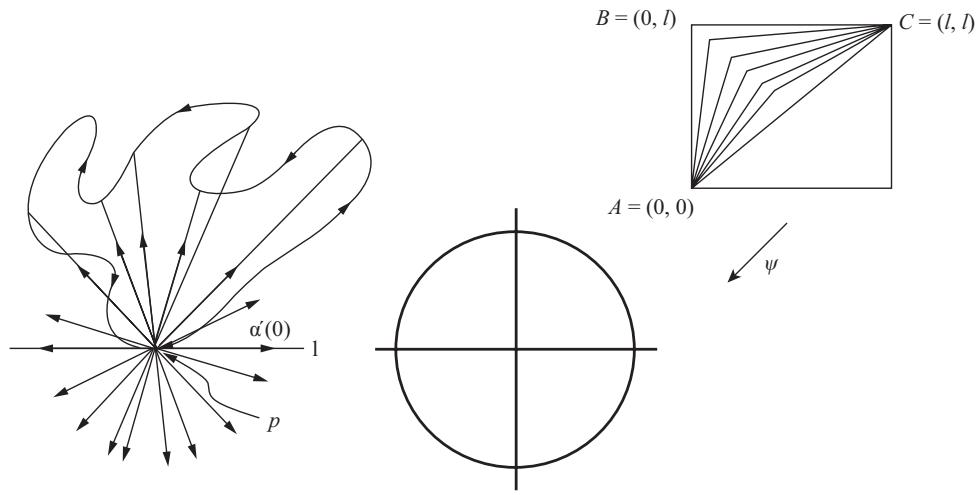
\includegraphics[width=\textwidth]{../../../PDFs/differential-geometry/transcript/Do Carmo - Differential Geometry of Curves and Surfaces/hybrid_ocr/images/ff9077e990e3e548a77e231dbb5f7e0360305761697ce26fb8d5c47ee3dc4524.jpg}}
\end{minipage}
\end{figure}

\begin{figure}[H]
\centering
\begin{minipage}{0.40\textwidth}
\centering
\subfloat[Figure 5-34. 凸曲线与非凸曲线]{\label{fig:fig5-34}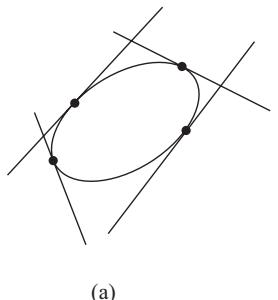
\includegraphics[width=\textwidth]{../../../PDFs/differential-geometry/transcript/Do Carmo - Differential Geometry of Curves and Surfaces/hybrid_ocr/images/4f62326d67117a93396ec49bcffc1e2770d5d5340c4d54977625e58e39a3351f.jpg}}
\end{minipage}
\end{figure}

\begin{figure}[H]
\centering
\begin{minipage}{0.40\textwidth}
\centering
\subfloat[Figure 5-34b]{\label{fig:fig5-34b}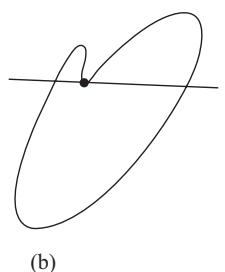
\includegraphics[width=\textwidth]{../../../PDFs/differential-geometry/transcript/Do Carmo - Differential Geometry of Curves and Surfaces/hybrid_ocr/images/c5d2a892ae88ef70ac20ac9d02a30174af8637a0770ae194e82b8da573858dce.jpg}}
\end{minipage}
\end{figure}

\begin{figure}[H]
\centering
\begin{minipage}{0.40\textwidth}
\centering
\subfloat[Figure 5-34c]{\label{fig:fig5-34c}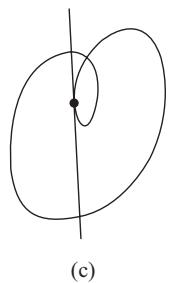
\includegraphics[width=\textwidth]{../../../PDFs/differential-geometry/transcript/Do Carmo - Differential Geometry of Curves and Surfaces/hybrid_ocr/images/09d205e5f688beb973c4e5df302e2742a68045f1a83427e32aa29da109efbb16.jpg}}
\end{minipage}
\end{figure}

\begin{figure}[H]
\centering
\begin{minipage}{0.40\textwidth}
\centering
\subfloat[Figure 5-35. 自交点破坏凸性]{\label{fig:fig5-35}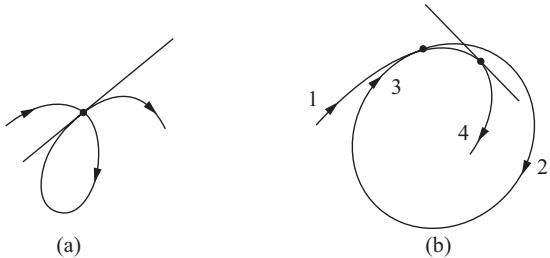
\includegraphics[width=\textwidth]{../../../PDFs/differential-geometry/transcript/Do Carmo - Differential Geometry of Curves and Surfaces/hybrid_ocr/images/301fce1bd36167de5f10051e2db69fe08e62dcb9bb26db2314ca2e3e9127ea2d.jpg}}
\end{minipage}
\end{figure}

\begin{figure}[H]
\centering
\begin{minipage}{0.40\textwidth}
\centering
\subfloat[Figure 5-36. 凸性证明中的矛盾构造]{\label{fig:fig5-36}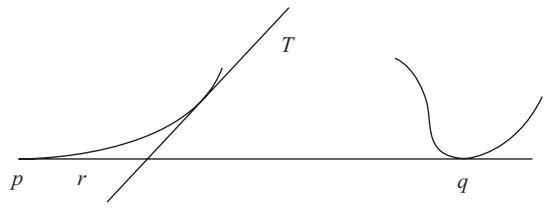
\includegraphics[width=\textwidth]{../../../PDFs/differential-geometry/transcript/Do Carmo - Differential Geometry of Curves and Surfaces/hybrid_ocr/images/ff2c420f27096383def9037990e840f80db1602bfa2351f44a7625fe209996f7.jpg}}
\end{minipage}
\end{figure}

\begin{figure}[H]
\centering
\begin{minipage}{0.40\textwidth}
\centering
\subfloat[Figure 5-37. Fenchel 定理证明中管状邻域的几何构造]{\label{fig:fig5-37}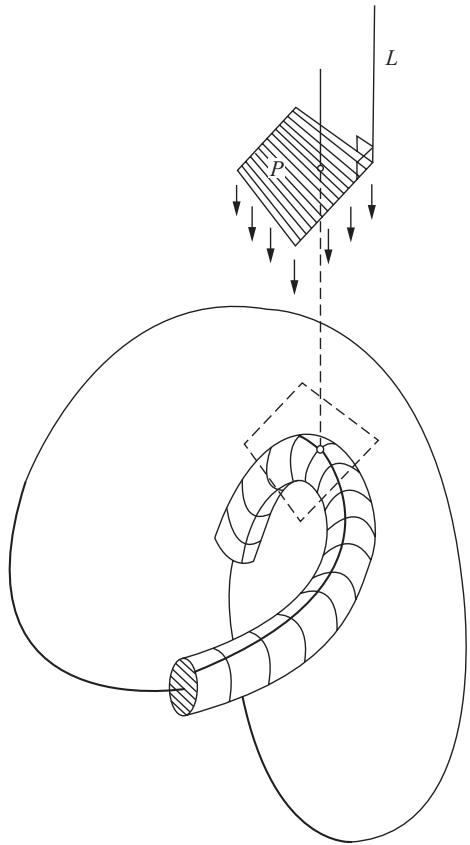
\includegraphics[width=\textwidth]{../../../PDFs/differential-geometry/transcript/Do Carmo - Differential Geometry of Curves and Surfaces/hybrid_ocr/images/b10384a4ea4291b1a46b38d15e25d867dd56ff3607bb59483260f473e0336b0e.jpg}}
\end{minipage}
\end{figure}

\begin{figure}[H]
\centering
\begin{minipage}{0.40\textwidth}
\centering
\subfloat[Figure 5-38. 打结与无结曲线]{\label{fig:fig5-38}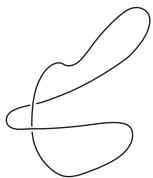
\includegraphics[width=\textwidth]{../../../PDFs/differential-geometry/transcript/Do Carmo - Differential Geometry of Curves and Surfaces/hybrid_ocr/images/cc8d2755ba12d4e524b5b863e724736f7b0565e5c8765003d3ed6f11a11db761.jpg}}
\end{minipage}
\end{figure}

\begin{figure}[H]
\centering
\begin{minipage}{0.40\textwidth}
\centering
\subfloat[Figure 5-38b]{\label{fig:fig5-38b}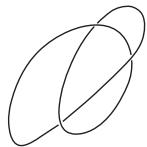
\includegraphics[width=\textwidth]{../../../PDFs/differential-geometry/transcript/Do Carmo - Differential Geometry of Curves and Surfaces/hybrid_ocr/images/7c390b78859dc6a0028aa3974709368e42b2bedcbe24214524ee276127fc4d33.jpg}}
\end{minipage}
\end{figure}

\begin{figure}[H]
\centering
\begin{minipage}{0.40\textwidth}
\centering
\subfloat[Figure 5-39. Fary-Milnor 定理证明中的平面束构造]{\label{fig:fig5-39}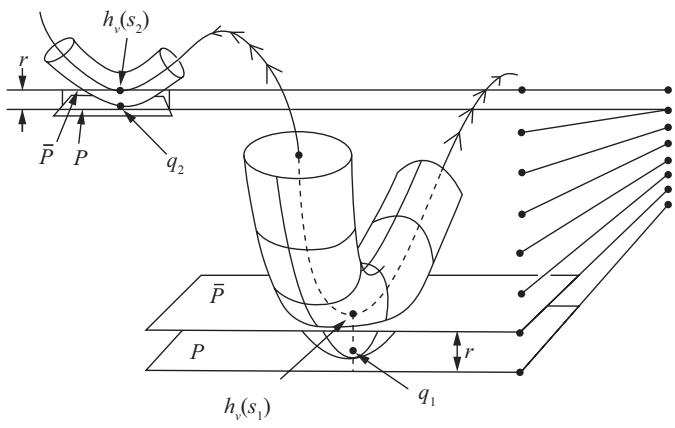
\includegraphics[width=\textwidth]{../../../PDFs/differential-geometry/transcript/Do Carmo - Differential Geometry of Curves and Surfaces/hybrid_ocr/images/ea583c8ab543401874ea889720250e99cb6bae539de50436e0b44b5e4896d9c0.jpg}}
\end{minipage}
\end{figure}

\begin{figure}[H]
\centering
\begin{minipage}{0.40\textwidth}
\centering
\subfloat[Figure 5-41. Schur 定理证明中的标准位置]{\label{fig:fig5-41}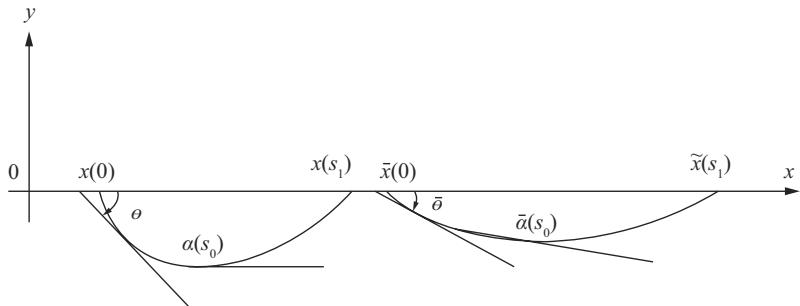
\includegraphics[width=\textwidth]{../../../PDFs/differential-geometry/transcript/Do Carmo - Differential Geometry of Curves and Surfaces/hybrid_ocr/images/f29131242ac5407089929a3b615272835cff52617ba4e6c570deefa6c2cbc25f.jpg}}
\end{minipage}
\end{figure}

\begin{figure}[H]
\centering
\begin{minipage}{0.40\textwidth}
\centering
\subfloat[Figure 5-42. Stoker 定理证明中的自交构造]{\label{fig:fig5-42}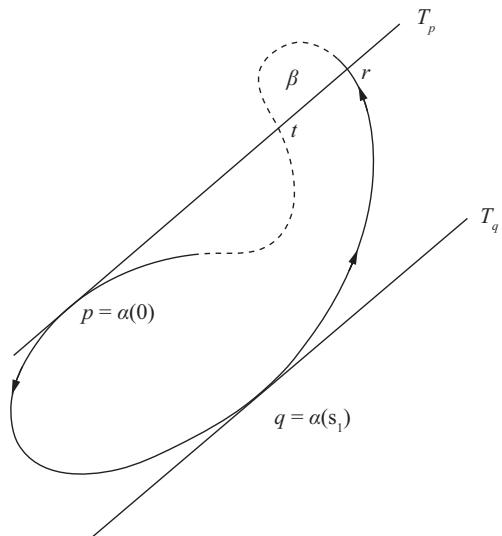
\includegraphics[width=\textwidth]{../../../PDFs/differential-geometry/transcript/Do Carmo - Differential Geometry of Curves and Surfaces/hybrid_ocr/images/57ba8397566cd9ae6bda0a674cae0cfb7444e72f650b980fd466fa1aa5b2ce48.jpg}}
\end{minipage}
\end{figure}

\begin{figure}[H]
\centering
\begin{minipage}{0.40\textwidth}
\centering
\subfloat[Figure 5-40. 旋转指标例题图]{\label{fig:fig5-40}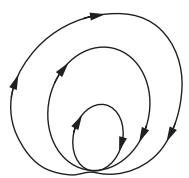
\includegraphics[width=\textwidth]{../../../PDFs/differential-geometry/transcript/Do Carmo - Differential Geometry of Curves and Surfaces/hybrid_ocr/images/b9ab02ccd8025ad6cf226231a05c30b8bf327b1950ee16c21367690f9b2d8106.jpg}}
\end{minipage}
\end{figure}

\begin{figure}[H]
\centering
\begin{minipage}{0.40\textwidth}
\centering
\subfloat[Figure 5-40b]{\label{fig:fig5-40b}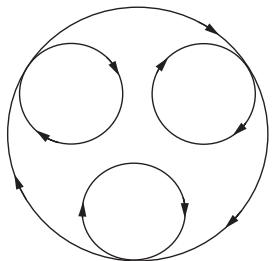
\includegraphics[width=\textwidth]{../../../PDFs/differential-geometry/transcript/Do Carmo - Differential Geometry of Curves and Surfaces/hybrid_ocr/images/664b9de0cf7db61c0e0d59db19bd8de089e9decbff3a0fce111d349301f37a55.jpg}}
\end{minipage}
\end{figure}

\begin{figure}[H]
\centering
\begin{minipage}{0.40\textwidth}
\centering
\subfloat[Figure 5-40c]{\label{fig:fig5-40c}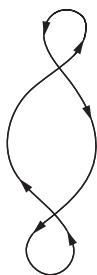
\includegraphics[width=\textwidth]{../../../PDFs/differential-geometry/transcript/Do Carmo - Differential Geometry of Curves and Surfaces/hybrid_ocr/images/4f11934b1993efab2b50ef9389661ec2455efd26c2a5343b555eefe58899d3cd.jpg}}
\end{minipage}
\end{figure}

\begin{figure}[H]
\centering
\begin{minipage}{0.40\textwidth}
\centering
\subfloat[Figure 5-40d]{\label{fig:fig5-40d}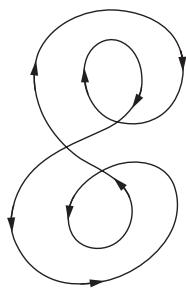
\includegraphics[width=\textwidth]{../../../PDFs/differential-geometry/transcript/Do Carmo - Differential Geometry of Curves and Surfaces/hybrid_ocr/images/bc4d8663ab8e4d6664173148f684c1540566475b92c15981142f217ff2698e32.jpg}}
\end{minipage}
\end{figure}

\begin{figure}[H]
\centering
\begin{minipage}{0.40\textwidth}
\centering
\subfloat[Figure 5-43. 零曲率曲面的构造例子：三角形加圆柱带]{\label{fig:fig5-43}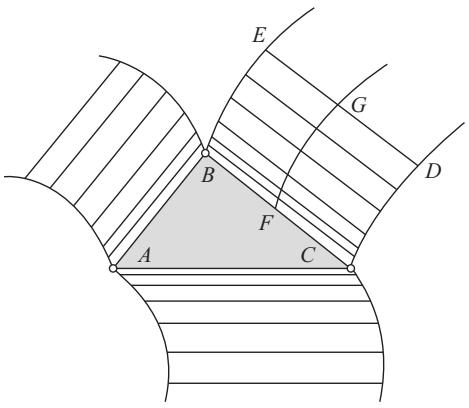
\includegraphics[width=\textwidth]{../../../PDFs/differential-geometry/transcript/Do Carmo - Differential Geometry of Curves and Surfaces/hybrid_ocr/images/b081fc47b2741c57cc08bf1ca3e3db4f8d4e4c7422dba00a30e4a926c5d53ff0.jpg}}
\end{minipage}
\end{figure}

\begin{Remark}
图 \cref{fig:fig5-30} 到 \cref{fig:fig5-43} 展示了本章各定理证明中的关键几何构造，请结合正文阅读。
\end{Remark}

\subsection*{5-6 节练习}

\begin{exercise}{5-6, 1 — do Carmo, Exercise 5-6, 1}
证明：映射 $\pi: \mathbb{R} \to S^1 = \{(x,y)\in\mathbb{R}^2: x^2+y^2=1\}$，$\pi(t) = (\cos t, \sin t)$，是覆叠映射。
\end{exercise}

\begin{exercise}{5-6, 2 — do Carmo, Exercise 5-6, 2}
证明：映射 $\pi: \mathbb{R}^2 - \{(0,0)\} \to \mathbb{R}^2 - \{(0,0)\}$，$\pi(x,y) = (x^2-y^2, 2xy)$，是双叶覆叠映射。
\end{exercise}

\begin{exercise}{5-6, 3 — do Carmo, Exercise 5-6, 3}
设 $S$ 是螺旋面（由螺旋线 $(\cos t, \sin t, bt)$ 的法向量生成），$L$ 是 $z$ 轴。设 $\pi: S - L \to \mathbb{R}^2 - \{(0,0)\}$ 为投影 $\pi(x,y,z) = (x,y)$。证明 $\pi$ 是覆叠映射。
\end{exercise}

\begin{exercise}{5-6, 4 — do Carmo, Exercise 5-6, 4}
证明：映射 $\pi: \mathbb{C} - \{0\} \to \mathbb{C} - \{0\}$，$\pi(z) = z^n$，是 $n$ 叶覆叠映射。
\end{exercise}

\begin{exercise}{5-6, 5 — do Carmo, Exercise 5-6, 5}
设 $B \subset \mathbb{R}^3$ 是弧道连通的。证明以下两个性质等价：
\begin{enumerate}
\item 对任意 $p,q \in B$ 和任意弧 $\alpha_0: [0,l] \to B$、$\alpha_1: [0,l] \to B$，存在 $B$ 中的同伦连接 $\alpha_0$ 到 $\alpha_1$；
\item 对任意 $p \in B$ 和任意闭弧 $\alpha: [0,l] \to B$（即 $\alpha(0) = \alpha(l) = p$），存在同伦将 $\alpha$ 连接到位常值弧 $\alpha(s) = p$（即对所有 $s$ 满足 $\alpha(s) = p$ 的常值弧）。
\end{enumerate}
\end{exercise}

\begin{exercise}{5-6, 6 — do Carmo, Exercise 5-6, 6}
设 $p_0 \in \mathbb{R}^2$，定义 $\varphi_t(p) = tp_0 + (1-t)p$。证明 $\mathbb{R}^2$ 是单连通的。
\end{exercise}

\begin{exercise}{5-6, 7a-b — do Carmo, Exercise 5-6, 7}
（a）利用球极投影和练习 6，证明 $S^2$ 上去掉至少一点的闭弧线与常值弧线同伦。（b）证明 $S^2$ 上任意闭弧线与去掉至少一点的闭弧线同伦。（c）由 (a)(b) 推出 $S^2$ 是单连通的。
\end{exercise}

\begin{exercise}{5-6, 8*（Klingenberg 引理）— do Carmo, Exercise 5-6, 8}
设 $S \subset \mathbb{R}^3$ 是高斯曲率 $K \leq K_0$（$K_0\geq 0$ 常数）的完备曲面。设 $p,q \in S$，$\gamma_0$ 和 $\gamma_1$ 是连接 $p$ 到 $q$ 的两条不同测地线，$l(\gamma_0) \leq l(\gamma_1)$，且 $\gamma_0$ 与 $\gamma_1$ 同伦。本题旨在证明：存在 $t_0 \in [0,1]$ 使得
\[
l(\gamma_0) + l(\alpha_{t_0}) \geq \frac{2\pi}{\sqrt{K_0}}.
\]
（因此，同伦必须经过一条"长"曲线。见图 \cref{fig:fig5-29}。）假设 $l(\gamma_0) < \pi/\sqrt{K_0}$（否则无需证明），按以下步骤进行：

\begin{enumerate}
\item[(a)] 利用第一比较定理（参见 5-5 节习题 3）证明 $\exp_p: T_p(S) \to S$ 在以 $p$ 为心、半径 $\pi/\sqrt{K_0}$ 的开圆盘 $B$ 内无临界点。
\item[(b)] 证明对小的 $t$，可以将曲线 $\alpha_t$ 提升到切平面 $T_p(S)$；即存在曲线 $\tilde{\alpha}_t$ 连接 $\exp_p^{-1}(p) = 0$ 到 $\exp_p^{-1}(q) = \tilde{q}$，使得 $\exp_p \circ \tilde{\alpha}_t = \alpha_t$。
\item[(c)] 证明 (b) 中的提升不能对所有 $t \in [0,1]$ 定义。由此推出对任意 $\epsilon > 0$，存在 $t(\epsilon)$ 使得 $\alpha_{t(\epsilon)}$ 可以提升为 $\tilde{\alpha}_{t(\epsilon)}$，且 $\tilde{\alpha}_{t(\epsilon)}$ 包含到 $B$ 边界距离小于 $\epsilon$ 的点。因此
\[
l(\gamma_0) + l(\alpha_{t(\epsilon)}) \geq \frac{2\pi}{\sqrt{K_0}} - 2\epsilon.
\]
\item[(d)] 在 (c) 中取一列 $\epsilon_n \to 0$，考虑 $\{t(\epsilon_n)\}$ 的收敛子序列。证明存在曲线 $\alpha_{t_0}$（$t_0 \in [0,1]$），使得
\[
l(\gamma_0) + l(\alpha_{t_0}) \geq \frac{2\pi}{\sqrt{K_0}}.
\]
\end{enumerate}
\end{exercise}

\begin{exercise}{5-6, 9a-b — do Carmo, Exercise 5-6, 9}
（a）利用 Klingenberg 引理证明：若 $S$ 是单连通、$K \geq 0$ 的完备曲面，则 $\exp_p: T_p(S) \to S$ 是单射。（b）用 (a) 给出 Hadamard 第一定理的简短证明。
\end{exercise}

\begin{exercise}{5-6, 10*（Synge 引理）— do Carmo, Exercise 5-6, 10}
回忆：曲面 $S$ 上的\textbf{可微闭曲线}是指可微映射 $\alpha: [0,l] \to S$，使得 $\alpha$ 及其所有导数在 $0$ 和 $l$ 处一致。两个可微闭曲线 $\alpha_0, \alpha_1: [0,l] \to S$ 是\textbf{自由同伦}的，如果存在连续映射 $H: [0,l] \times [0,1] \to S$ 使得 $H(s,0) = \alpha_0(s)$，$H(s,1) = \alpha_1(s)$，$s \in [0,l]$。映射 $H$ 称为 $\alpha_0$ 和 $\alpha_1$ 之间的\textbf{自由同伦}（端点不固定）。

设 $S$ 定向且 $K>0$。证明：$S$ 上任意简单闭测地线与更短闭曲线自由同伦。
\end{exercise}

\begin{exercise}{5-6, 11 — do Carmo, Exercise 5-6, 11}
设 $S$ 是单连通完备曲面，$p$ 是 $S$ 的极点（即从 $p$ 出发的任意测地线均无共轭点）。利用 Klingenberg 引理的技术证明：$\exp_p: T_p(S) \to S$ 是微分同胚。
\end{exercise}

% ==================== Section 5-7: Global Theorems for Curves: The Fary-Milnor Theorem ====================
\section{Global Theorems for Curves: The Fary-Milnor Theorem}\label{sec:fary-milnor}

本节研究闭曲线的整体性质，主要工具是连续映射的度（degree）理论。

\textbf{度的概念.} 设 $\pi: \mathbb{R} \to S^1$，$\pi(x) = (\cos x, \sin x)$ 是覆叠映射。对连续映射 $\varphi: S^1 \to S^1$，取闭合弧 $\varphi: [0,l] \to S^1$，提升为 $\tilde{\varphi}: [0,l] \to \mathbb{R}$，则 $\tilde{\varphi}(l) - \tilde{\varphi}(0) = 2\pi\cdot\deg\varphi$，其中整数 $\deg\varphi$ 称为 $\varphi$ 的\textbf{度}——即 $\varphi$ 绕 $S^1$ 的"圈数"。

\textbf{度的不变性.} 同伦的映射有相同的度。

\textbf{旋转指标.} 正则平面闭曲线 $\alpha: [0,l] \to \mathbb{R}^2$ 的切映射 $\varphi(t) = \alpha'(t)/|\alpha'(t)|$ 的度称为该曲线的\textbf{旋转指标}（rotation index）。它表示切向量沿曲线绕行的总圈数。

\begin{Theorem}[可微 Jordan 曲线定理]\label{differentiable-jordan}
设 $\alpha: [0,l] \to \mathbb{R}^2$ 是正则、简单、闭平面曲线。则 $\mathbb{R}^2 - \alpha([0,l])$ 恰好有两个连通分支，$\alpha([0,l])$ 是它们的公共边界。
\end{Theorem}

\begin{Theorem}[旋转定理]\label{rotation-index}
设 $\beta: [0,l] \to \mathbb{R}^2$ 是正则、简单、闭平面曲线。则 $\beta$ 的旋转指标为 $\pm 1$（取决于定向）。
\end{Theorem}

\textbf{凸曲线的特征.}

\begin{Proposition}\label{prop:convex-curve}
正则、闭平面曲线是凸的，当且仅当它简单且曲率 $k$ 不变号。
\end{Proposition}

\begin{Remark}
曲率 $k$ 不变号 $\Leftrightarrow$ 旋转指标为 $\pm 1$ 且曲线无自交 $\Leftrightarrow$ 曲线是凸的。
\end{Remark}

\textbf{Fenchel 定理（总曲率的下界）.}

\begin{Theorem}[Fenchel 定理]\label{fenchel}
简单闭空间曲线的全曲率 $\geq 2\pi$，等号成立当且仅当该曲线是平面凸曲线。
\end{Theorem}

\textbf{证明概要.} 设 $T$ 是曲线 $\alpha$ 半径为 $r$ 的管状邻域（$r$ 足够小），$R \subset T$ 是 $K \geq 0$ 的区域。直接计算
\[
\iint_R K\,d\sigma = 2\int_0^l k(s)\,ds = 2\cdot(\text{总曲率}).
\]
另一方面，每个单位向量恰好作为法方向在 $R$ 中出现至少一次（因为任意方向都垂直于某支持平面），故 $\iint_R K\,d\sigma \geq 4\pi$。于是总曲率 $\geq 2\pi$。等号情况对应所有法方向恰好出现一次，即曲线为平面凸曲线。\footnote{详细推导见附录 \cref{sec:derivation-fenchel}}

\textbf{Fary-Milnor 定理（打结曲线的更多曲率）.}

\begin{Theorem}[Fary-Milnor]\label{fary-milnor}
若简单闭空间曲线是打结的（knotted），则其全曲率 $> 4\pi$。
\end{Theorem}

直观含义：打结使曲线的最少总曲率从 $2\pi$ 增加到 $>4\pi$——打结需要额外的"空间"来容纳。

\begin{Remark}
Fenchel 定理和 Fary-Milnor 定理是曲线理论中最重要的整体结果。它们表明曲线的"缠绕方式"（拓扑）与曲线的弯曲程度（几何）之间存在深刻的量化联系。
\end{Remark}

\begin{Remark}
打结与无结的分类（纽结理论）是拓扑学的重要分支。Fary-Milnor 定理是微分几何与拓扑学交叉的经典范例：曲率下界 $>4\pi$ 是曲线打结的几何判据。
\end{Remark}

\begin{Remark}
历史上，Fenchel 定理首先由 Fenchel 证明（1929），Fary 和 Milnor 分别独立得到更强的 $>4\pi$ 估计。
\end{Remark}

\begin{Remark}
定理 \ref{rotation-index}（旋转定理）是 Gauss-Bonnet 定理应用于平面曲线时的核心应用之一，它说明平面凸曲线的旋转指标恒为 $\pm 1$，与曲线的具体形状无关。
\end{Remark}

\begin{Remark}
定理 \ref{differentiable-jordan} 是 Jordan 曲线定理的可微版本（经典 Jordan 定理只要求曲线是连续的）。利用管状邻域和卷绕数的概念，可以给出简洁的可微情形证明。
\end{Remark}

\begin{Remark}
定理 \ref{fary-milnor} 的证明用到了管状邻域上的 Gauss-Bonnet 定理（应用于管面的曲率积分）与几何对偶性（单位球面上法方向的覆盖次数）。
\end{Remark}

\begin{Remark}
椭圆面（ellipsoid）的共轭轨迹见 \cref{fig:fig5-19}。这是一般曲面的典型行为：共轭点沿一条曲线分布，而不像球面那样缩约成唯一点。
\end{Remark}

\begin{Remark}
第 5-7 节的全部内容仅依赖于第 5-6 节 A 部分（覆叠空间基础），不需要 Hadamard 定理本身。这使得本节在依赖关系上相对独立。
\end{Remark}

\begin{Remark}
度的理论在微分几何中有广泛应用：Gauss-Bonnet 定理中向量场的指数和（第 4-5 节）、测地线的个数问题，以及后续课程中的微分形式与上同调等。
\end{Remark}

\begin{Remark}
凸曲线的内域是凸集（命题 \ref{prop:convex-curve} 的几何推论），这与直觉一致：凸曲线围成的区域没有"凹陷"。
\end{Remark}

\begin{Remark}
本节的许多定理依赖于覆盖空间理论（第 5-6 节 A 部分）所提供的拓扑工具。这是本书中拓扑方法在微分几何中的又一次成功应用。
\end{Remark}

\begin{Remark}
Fenchel 定理的另一个等价表述：任意闭曲线的全曲率不小于 $2\pi$，等号当且仅当曲线是平面凸曲线。这一简洁的不等式蕴含了深刻的几何拓扑内容。
\end{Remark}

\begin{Remark}
关于凸性的另一种刻画：若正则闭曲线是某凸集的边界，则它必为凸曲线。反之，凸曲线的内域必为凸集。
\end{Remark}

\begin{Remark}
定理 \ref{fary-milnor} 中 " $>4\pi$" 的出现可以从管状邻域的几何理解：管面的高斯曲率积分给出 $2\int k\,ds$，而打结曲线的法方向在单位球面上覆盖至少两次（对应旋转指标 $\geq 2$），从而积分值加倍。
\end{Remark}

\begin{Remark}
若将曲线全曲率的上确界设为无穷（无界曲线），则 Fary-Milnor 定理说明：打结曲线的弯曲程度有非零下界——这体现了拓扑约束对几何量的控制。
\end{Remark}

\begin{Remark}
第 5-7 节的练习涵盖了旋转指标、卷绕数、同伦不变性、Stoker 定理等丰富内容，是理解整体曲线理论的重要素材。
\end{Remark}

\begin{Remark}
球面上无零挠率的正则闭曲线（Stoker 定理的一个特例）满足全挠率为零：$\int_0^l \tau(s)\,ds = 0$。这是球面几何的另一个有趣的整体约束。
\end{Remark}

\begin{Remark}
Schur 定理（练习 7）说明了曲率大小与弦长之间的单调关系：若两条等长平面凸曲线的曲率处处满足 $k \geq \tilde{k}$，则对应的弦长有 $d \geq \tilde{d}$——这体现了"更弯的曲线更短"这一直观事实。
\end{Remark}

\begin{Remark}
本节的核心工具——度的理论——在现代数学（代数拓扑、微分拓扑）中有着根本的重要性，其应用远远超出本章范围。
\end{Remark}

\begin{Remark}
图 \cref{fig:fig5-30} 到 \cref{fig:fig5-42} 展示了度的概念、旋转定理、凸曲线刻画、Fenchel 定理和 Fary-Milnor 定理证明中的关键几何构造。
\end{Remark}

\begin{Remark}
第 5-7 节的内容与第 5-6 节 A 部分紧密相关：度的理论建立在覆叠空间（特别是 $\mathbb{R} \to S^1$）之上，而 Jordan 曲线定理和旋转定理则为 Gauss-Bonnet 定理（平面曲线情形）提供了几何基础。
\end{Remark}

\begin{Remark}
本章第 5-7 节展示了整体微分几何的一个核心主题：利用局部几何量（曲率、挠率）和整体拓扑假设（简单性、同伦类）来建立曲线和曲面的深刻性质。这些思想在黎曼几何中得到了系统的发展。
\end{Remark}

\begin{Remark}
特别值得强调的是 Hadamard 定理（定理 \ref{hadamard-first} 和 \ref{hadamard-second}）：它们建立了曲率符号（$K \leq 0$ 或 $K>0$）与曲面整体拓扑类型（平面型或球面型）之间的一一对应，是整体微分几何最漂亮的结果之一。
\end{Remark}

\begin{Remark}
第 5-7 节与第 5-5 节（Jacobi 场）和第 5-4 节（变分）密切相关：Fenchel 定理的证明本质上利用了管状邻域的变分性质，而 Jacobi 场的理论为共轭点提供了分析框架。
\end{Remark}

\begin{Remark}
Bonnet 定理（定理 \ref{bonnet}）的证明是本课程中最复杂的变分计算之一：第二变分公式（命题 \ref{prop:second-variation}）结合精心构造的变分场（$V(s) = w(s)\sin\frac{\pi}{l}s$）给出关键的不等式，揭示了正曲率"压缩"测地线的几何机制。
\end{Remark}

\begin{Remark}
Hopf-Rinow 定理（定理 \ref{hopf-rinow}）是完备曲面理论的基石：它保证完备曲面上任意两点间存在最小测地线，这一存在性是后续所有整体定理的第一步。
\end{Remark}

\begin{Remark}
球面刚性定理（定理 \ref{sphere-rigidity}）是本章第一个整体定理，其证明方法（引理 \ref{sphere-lemma1} 利用 Mainardi-Codazzi 方程）成为后续曲面论研究的标准技术。
\end{Remark}

\begin{Remark}
本章的整体定理有一个共同模式：局部几何量（曲率） + 整体假设（完备性/紧致性/单连通） $\Longrightarrow$ 强整体结论。这些定理体现了微分几何的核心思想：内蕴几何性质与整体拓扑之间的深刻联系。
\end{Remark}

\begin{Remark}
本章的各节内容相互依存：5-3 节（完备性） $\to$ 5-4 节（Bonnet） $\to$ 5-5 节（Jacobi 场） $\to$ 5-6 节（Hadamard）形成一条主线，最终在 5-8 节（零曲率曲面）和 5-11 节（Hilbert 定理）中得到更多应用。
\end{Remark}

\begin{Remark}
除主线外，本章还包含两条独立线索：5-2 节（球面刚性）和 5-7 节（曲线整体定理），它们各自依赖较少，可单独学习。
\end{Remark}

\begin{Remark}
第 5-10 节（抽象曲面）引入的抽象曲面概念（即不理嵌入 $\mathbb{R}^3$ 的曲面）是向流形概念的重要过渡，它表明内蕴几何的核心概念（第一基本形式、测地线、完备性）可以在更抽象的框架中定义和研究。
\end{Remark}

\begin{Remark}
Hilbert 定理（定理 \ref{hilbert-theorem}）是整体微分几何最著名的"不可能定理"之一：它断言 $\mathbb{R}^3$ 中不存在常负曲率的完备正则曲面。这引导了 $\mathbb{R}^3$ 中负曲率曲面的研究——以及黎曼几何中双曲空间的发现。
\end{Remark}

\begin{Remark}
本章的拓扑附录（点集拓扑）为正文提供了必要的拓扑基础，包括连通性、紧致性、弧道连通性和同伦等概念的形式定义与证明，确保本书的自洽性。
\end{Remark}

\begin{Remark}
本章最后的习题集涵盖了各节的核心内容，其中标记 * 的为较难题目。特别推荐：5-3 节练习 11（Osserman 引理——极小曲面完备性的深刻障碍）和 5-5 节练习 3（比较定理——Jacobi 场理论的核心应用）。
\end{Remark}

% ==================== Exercises 5-7 ====================
\begin{exercise}{5-7, 1 — do Carmo, Exercise 5-7, 1}
Determine the rotation indices of curves (a), (b), (c), and (d) in Fig. 5-40.
\end{exercise}

\begin{exercise}{5-7, 2 — do Carmo, Exercise 5-7, 2}
Let $\alpha(t) = (x(t), y(t))$, $t \in [0, l]$, be a differentiable plane closed curve. Let $p_0 = (x_0, y_0) \in R^2$, $(x_0, y_0) \notin \alpha([0, l])$, and define the functions

$$
a (t) = \frac {x (t) - x _ {0}}{\left\{(x (t) - x _ {0}) ^ {2} + (y (t) - y _ {0}) ^ {2} \right\} ^ {1 / 2}},
$$

$$
b (t) = \frac {y (t) - y _ {0}}{\{(x (t) - x _ {0}) ^ {2} + (y (t) - y _ {0}) ^ {2} \} ^ {1 / 2}}.
$$

a. Use Lemma 1 of Sec. 4-4 to show that the differentiable function

$$
\varphi (t) = \varphi_ {0} + \int_ {0} ^ {t} \left(a b ^ {\prime} - b a ^ {\prime}\right) d t, \quad a ^ {\prime} = \frac {d a}{d t}, b ^ {\prime} = \frac {d b}{d t},
$$

is a determination of the angle that the $x$ axis makes with the position vector $(\alpha(t) - p_0) / |\alpha(t) - p_0|$.

b. Use part a to show that when $\alpha$ is a differentiable closed plane curve, the winding number of $\alpha$ relative to $p_0$ is given by the integral

$$
w = \frac {1}{2 \pi} \int_ {0} ^ {l} (a b ^ {\prime} - b a ^ {\prime}) d t.
$$
\end{exercise}

\begin{exercise}{5-7, 3 — do Carmo, Exercise 5-7, 3}
Let $\alpha \colon [0,l] \to R^2$ and $\beta \colon [0,l] \to R^2$ be two differentiable plane closed curves, and let $p_0 \in R^2$ be a point such that $p_0 \notin \alpha([0,l])$ and $p_0 \notin \beta([0,l])$. Assume that, for each $t \in [0,l]$, the points $\alpha(t)$ and $\beta(t)$ are closer than the points $\alpha(t)$ and $p_0$; i.e.,

$$
| \alpha (t) - \beta (t) | < | \alpha (t) - p _ {0} |.
$$

Use Exercise 2 to prove that the winding number of $\alpha$ relative to $p_0$ is equal to the winding number of $\beta$ relative to $p_0$.
\end{exercise}

\begin{exercise}{5-7, 4 — do Carmo, Exercise 5-7, 4}
a. Let $C$ be a regular plane closed convex curve. Since $C$ is simple, it determines, by the Jordan curve theorem, an interior region $K \subset R^2$. Prove that $K$ is a convex set (i.e., given $p, q \in K$, the segment of straight line $\overline{pq}$ is contained in $K$; cf. Exercise 9, Sec. 1-7).

b. Conversely, let $C$ be a regular plane curve (not necessarily closed), and assume that $C$ is the boundary of a convex region. Prove that $C$ is convex.
\end{exercise}

\begin{exercise}{5-7, 5 — do Carmo, Exercise 5-7, 5}
Let $C$ be a regular plane, closed, convex curve. By Exercise 4, the interior of $C$ is a convex set $K$. Let $p_0 \in K$, $p_0 \notin C$.

a. Show that the line which joins $p_0$ to an arbitrary point $q \in C$ is not tangent to $C$ at $q$.
b. Conclude from part a that the rotation index of $C$ is equal to the winding number of $C$ relative to $p_0$.
c. Obtain from part b a simple proof for the fact that the rotation index of a closed convex curve is $\pm 1$.
\end{exercise}

\begin{exercise}{5-7, 6 — do Carmo, Exercise 5-7, 6}
Let $\alpha \colon [0, l] \to R^3$ be a regular closed curve parametrized by arc length. Assume that $0 \neq |k(s)| \leq 1$ for all $s \in [0, l]$. Prove that $l \geq 2\pi$ and that $l = 2\pi$ if and only if $\alpha$ is a plane convex curve.
\end{exercise}

\begin{exercise}{5-7, 7 — do Carmo, Exercise 5-7, 7 (Schur's Theorem for Plane Curves)}
Let $\alpha$ : $[0, l] \to R^2$ and $\tilde{\alpha}$ : $[0, l] \to R^2$ be two plane convex curves parametrized by arc length, both with the same length $l$. Denote by $k$ and $\tilde{k}$ the curvatures of $\alpha$ and $\tilde{\alpha}$, respectively, and by $d$ and $\tilde{d}$ the lengths of the chords of $\alpha$ and $\tilde{\alpha}$, respectively; i.e.,

$$
d (s) = | \alpha (s) - \alpha (0) |, \quad \tilde {d} (s) = | \tilde {\alpha} (s) - \tilde {\alpha} (0) |.
$$

Assume that $k(s) \geq \tilde{k}(s)$, $s \in [0, l]$. We want to prove that $d(s) \leq \tilde{d}(s)$, $s \in [0, l]$ (i.e., if we stretch a curve, its chords become longer) and that equality holds for $s \in [0, l]$ if and only if the two curves differ by a rigid motion. We remark that the theorem can be extended to the case where $\tilde{\alpha}$ is a space curve and has a number of applications, Compare S. S. Chern [10].

The following outline may be helpful.

a. Fix a point $s = s_1$. Put both curves $\alpha(s) = (x(s), y(s))$, $\tilde{\alpha}(s) = (\tilde{x}(s), \tilde{y}(s))$ in the lower half-plane $y \leq 0$ so that $\alpha(0), \alpha(s_1), \tilde{\alpha}(0)$, and $\tilde{\alpha}(s_1)$ lie on the $x$ axis and $x(s_1) > x(0)$, $\tilde{x}(s_1) > \tilde{x}(0)$ (see Fig. 5-41). Let $s_0 \in [0, s_1]$ be such that $\alpha'(s_0)$ is parallel to the $x$ axis. Choose the function $\theta(s)$ which gives a differentiable determination of the angle that the $x$ axis makes with $\alpha'(s)$ in such a way that $\theta(s_0) = 0$. Show that, by convexity, $-\pi \leq \theta \leq \pi$.

b. Let $\tilde{\theta}(s)$, $\tilde{\theta}(s_0) = 0$, be a differentiable determination of the angle that the $x$ axis makes with $\alpha'(s)$. (Notice that $\tilde{\alpha}'(s_0)$ may no longer be parallel to the $x$ axis.) Prove that $\tilde{\theta}(s) \leq \theta(s)$ and use part a to conclude that

$$
d \left(s _ {1}\right) = \int_ {0} ^ {s _ {1}} \cos \theta (s) d s \leq \int_ {0} ^ {s _ {1}} \cos \tilde {\theta} (s) d s \leq \tilde {d} \left(s _ {1}\right).
$$

For the equality case, just trace back your steps and apply the uniqueness theorem for plane curves.
\end{exercise}

\begin{exercise}{5-7, 8 — do Carmo, Exercise 5-7, 8 (Stoker's Theorem for Plane Curves)}
Let $\alpha \colon R \to R^2$ be a regular plane curve parametrized by arc length. Assume that $\alpha$ satisfies the following conditions:

1. The curvature of $\alpha$ is strictly positive.
2. $\lim_{s\to \pm \infty}|\alpha (s)| = \infty$; that is, the curve extends to infinity in both directions.
3. $\alpha$ has no self-intersections.

The goal of the exercise is to prove that the total curvature of $\alpha$ is $\leq \pi$.

The following indications may be helpful. Assume that the total curvature is $> \pi$ and that $\alpha$ has no self-intersections. To obtain a contradiction, proceed as follows:

a. Prove that there exist points, say, $p = \alpha(0)$, $q = \alpha(s_1)$, $s_1 > 0$, such that the tangent lines $T_p$, $T_q$ at the points $p$ and $q$, respectively, are parallel and there exists no tangent line parallel to $T_p$ in the arc $\alpha([0, s_1])$.
b. Show that as $s$ increases, $\alpha(s)$ meets $T_p$ at a point, say, $r$ (Fig. 5-42).
c. The arc $\alpha ((-\infty ,0))$ must meet $T_{p}$ at a point $t$ between $p$ and $r$.
d. Complete the arc $tpqr$ of $\alpha$ with an arc $\beta$ without self-intersections joining $r$ to $t$, thus obtaining a closed curve $C$. Show that the rotation index of $C$ is $\geq 2$. Show that this implies that $\alpha$ has self-intersections, a contradiction.
\end{exercise}

\begin{exercise}{5-7, 9* — do Carmo, Exercise 5-7, 9}
Let $\alpha \colon [0, l] \to S^2$ be a regular closed curve on a sphere $S^2 = \{(x, y, z) \in R^3; x^2 + y^2 + z^2 = 1\}$. Assume that $\alpha$ is parametrized by arc length and that the curvature $k(s)$ is nowhere zero. Prove that

$$
\int_ {0} ^ {l} \tau (s) d s = 0.
$$
\end{exercise}

% ==================== Section 5-8: Surfaces of Zero Gaussian Curvature ====================
\section{Surfaces of Zero Gaussian Curvature}\label{sec:zero-gaussian-curvature}

我们已经知道（第 4-6 节）高斯曲率恒为零的正则曲面局部等距于平面。本节研究它们在 $\mathbb{R}^3$ 中的整体形状。

\begin{Theorem}\label{zero-curvature-surface}
设 $S \subset \mathbb{R}^3$ 是高斯曲率 $K \equiv 0$ 的完备曲面。则 $S$ 是一张平面或一根圆柱面。
\end{Theorem}

\textbf{圆柱面的定义.} 圆柱面是指：过每点 $p \in S$ 有唯一一条直线（称为该点的\textbf{母线}，generator），且任意两条不同母线平行或重合的正则曲面。

\textbf{证明思路.} 设 $P$ 为 $S$ 的平面点（planar points，即 $H=0$ 的点），$U = S - P$ 为抛物点（parabolic points）。先证明：过每抛物点存在唯一的渐近曲线，且它是直线段。若这条直线无限延伸，它永不能与 $P$ 相交——从而要么无界（平面的一部分），要么闭合（圆柱面）。

\textbf{关键引理.} 设 $p \in U$ 是抛物点。则过 $p$ 的唯一渐近曲线（也是法曲率为零的曲线）是直线段（命题 1）。利用 Mainardi-Codazzi 方程可证：沿该渐近曲线，主曲率 $k_1 = 0$，$k_2$ 不变号。

\begin{Lemma}\label{zero-curvature-asymptotic}
设 $p \in U$ 是抛物点，则过 $p$ 的渐近曲线是直线段。
\end{Lemma}

\begin{Proof}[证明概要]
在曲率线坐标下，渐近曲线 $v=\mathrm{const}$ 满足 $e=0$，从而 $N_u=0$ 沿该曲线。由 Mainardi-Codazzi 方程可推出 $\langle \mathbf{x}, N\rangle = \varphi(v)$，结合 $N_v \neq 0$ 可知曲线同时位于两张不同平面的交集中，故为直线段。\footnote{详细推导见附录 \cref{sec:derivation-zero-curvature-asymptotic}}
\end{Proof}

\textbf{Example（零曲率曲面构造）.} \cref{fig:fig5-43} 展示了一个 $K \equiv 0$ 曲面的构造：由开三角形 $ABC$ 的每条边加上与之平行的圆柱带构成。注意平面点（三角形内部）的边界（各边）是渐近曲线（直线段），而圆柱带上的点是抛物点。$P$ 在 $S$ 中闭，但不在 $\mathbb{R}^3$ 中闭。

\begin{Remark}
该定理的完整证明比较复杂，涉及 Mainardi-Codazzi 方程的精细估计。直观上：$K=0$ 意味着第二基本形式的行列式为零——每个点要么是平面点（两个主曲率均为零），要么是抛物点（一个主曲率为零，另一个非零）。抛物点的渐近方向唯一确定了一条直线段。
\end{Remark}

\begin{Remark}
该结果首先由 P. Hartman 和 L. Nirenberg (1959) 得到，之后 W. S. Massey (1962) 和 J. J. Stoker (1961) 给出了更简洁的证明。本证明遵循 Massey 的方法。
\end{Remark}

\begin{Remark}
定理 \ref{zero-curvature-surface} 的结论不能加强：存在非平面非圆柱面的完备 $K=0$ 曲面（如上例的构造）。要得到平面或圆柱面，$K \equiv 0$ 和完备性都是必要的。
\end{Remark}

\begin{Remark}
该定理也是 Bonnet 定理（第 5-4 节）的推论的推论：当 $K \geq \delta > 0$ 时曲面紧致；当 $K \leq 0$ 时曲面有特殊拓扑；而 $K \equiv 0$ 则直接决定了曲面是平面或圆柱面。
\end{Remark}

\begin{Remark}
该定理的几何意义：若一个曲面没有"内在弯曲"（$K=0$）且在所有方向上完备，则它只能是一片平面或一根管状曲面（圆柱面）。
\end{Remark}

\begin{Remark}
历史上，这一结果来得很晚——直到 1959 年才被证明，而高斯曲率的概念早在十九世纪初就已经确立了。这说明了整体微分几何的困难程度：局部理论相对简单，但要理解曲面的整体行为需要更深厚的分析工具。
\end{Remark}

\begin{Remark}
定理 \ref{zero-curvature-surface} 也是 Hadamard 定理（第 5-6 节）的类比：$K<0$ 的完备单连通曲面微分同胚于平面；$K\equiv 0$ 的完备曲面则平面或圆柱面。这些都是曲率条件决定整体拓扑的经典范例。
\end{Remark}

\begin{Remark}
Massey 的证明思想后来被推广到更一般的情形（Stoker 的工作），成为整体曲面论中的重要技术。
\end{Remark}

\begin{Remark}
圆柱面（$K=0$）与平面（也是 $K=0$）的一个重要区别：平面是单连通的，而圆柱面的基本群为 $\mathbb{Z}$。但两者都是 $K=0$ 的例子——这说明 $K$ 的信息不足以区分所有拓扑类型。
\end{Remark}

\begin{Remark}
将本节结果与第 3-3 节旋转面理论结合：旋转面中 $K=0$ 的面（除平面外）就是圆柱面——这是本定理在旋转面类中的特例。
\end{Remark}

\begin{Remark}
该定理也是研究高斯曲率符号与曲面拓扑关系的里程碑：$K>0$（球面/卵形面）、$K\equiv 0$（平面/圆柱面）、$K<0$（平面型/双曲型）——三种曲率情形对应三种整体拓扑类型。
\end{Remark}

\begin{Remark}
定理 \ref{zero-curvature-surface} 在物理中也有应用：$K=0$ 的曲面在弹性理论（薄壳理论）和计算机图形学（曲面建模）中都有特殊地位。
\end{Remark}

\begin{Remark}
注：在 2016 年的修订版中，作者引用了 A. V. Pogorelov (1956) 的一份早期工作，说明该结果实际上更早由 Pogorelov 得到。
\end{Remark}

\begin{Remark}
本节内容的核心是 Mainardi-Codazzi 方程在 $K=0$ 条件下的特殊形式，这一方程在第 4-3 节引入，是曲面论的基石之一。
\end{Remark}

\begin{Remark}
值得注意的是，$K \equiv 0$ 的曲面虽然"平坦"（无内蕴曲率），但作为 $\mathbb{R}^3$ 中的子曲面仍然可以有非平凡的形状（圆柱面、锥面等）——这体现了内蕴几何（第一基本形式）与外在几何（作为 $\mathbb{R}^3$ 中的曲面）的区别。
\end{Remark}

\begin{Remark}
本节的结论不能推广到更高维：黎曼几何中，$n$ 维完备平坦流形可以是环面等（晶体群商），而不一定是欧氏空间。这使得二维情形更加特殊和漂亮。
\end{Remark}

\begin{Remark}
本节习题涉及零曲率曲面与平面和圆柱面之间的内在联系，以及 Mainardi-Codazzi 方程在特殊条件下的应用。
\end{Remark}

\begin{Remark}
本节内容依赖于第 5-3、5-4、5-5 节和第 5-6 节 A 部分，与第 5-7 节和第 5-9 到 5-11 节基本独立。
\end{Remark}

\begin{Remark}
第 5-8 节的结果将在第 5-11 节（Hilbert 定理）的证明中再次用到：通过证明完备负曲率曲面不能嵌入 $\mathbb{R}^3$，Hilbert 建立了 $K<0$ 与 $K \equiv 0$ 情形之间的深刻区别。
\end{Remark}

\begin{Remark}
本节定理的一个直接推论：若 $S$ 是 $K=0$ 的完备曲面且包含一个平面点（$H=0$ 的椭圆点），则 $S$ 必须是平面——因为过平面点的渐近曲线（直线）不能与自身相交。
\end{Remark}

\begin{Remark}
该定理在微分几何课程中通常被视为"收官"内容——它综合运用了曲面论、变分法和拓扑工具，展示了整体微分几何的完整力量。
\end{Remark}

\begin{Remark}
从历史角度，该定理的姗姗来迟反映了整体微分几何的困难：局部理论（由高斯开创）在十九世纪已相当成熟，但整体结果的获得需要二十世纪的新思想和新工具（变分法、拓扑学、偏微分方程）。
\end{Remark}

\begin{Remark}
本节标题中的"曲面"指嵌入 $\mathbb{R}^3$ 中的正则曲面。第 5-10 节将把类似概念推广到抽象曲面（不依赖嵌入），从而建立更一般的黎曼几何框架。
\end{Remark}

\begin{Remark}
从本节定理可以引出一个有趣的问题：$K=0$ 的完备曲面在等距变换下的分类问题。答案就是本定理所述的平面或圆柱面——这是平面上刚体运动群在 $\mathbb{R}^3$ 中的实现。
\end{Remark}

\begin{Remark}
读者若对零曲率曲面感兴趣，可进一步阅读：平移曲面（translation surfaces）、极小曲面（极小曲面的高斯曲率也满足特殊方程）等研究方向。
\end{Remark}

\begin{Remark}
本节证明中使用的 Mainardi-Codazzi 方程在 $K=0$ 时的简化形式 $(e_v = \frac{E_v}{2}(k_1+k_2))$ 等，是处理这类问题的标准工具，读者应熟练掌握。
\end{Remark}

\begin{Remark}
需要特别强调的是，本节定理中的完备性假设至关重要：去掉完备性，$K=0$ 的正则曲面可以是任意形状的局部平面区域。
\end{Remark}

\begin{Remark}
从本定理还可推出：完备 $K=0$ 曲面在 $\mathbb{R}^3$ 中的等距刚性问题已经有完整分类——这与球面的刚性定理（第 5-2 节）形成鲜明对比。
\end{Remark}

\begin{Remark}
本节的最后，值得指出的是：$K=0$ 的曲面虽然局部等距于平面，但其作为 $\mathbb{R}^3$ 中的子曲面的行为却有本质差异——平面是自共轭的（法向量场平行），而圆柱面有非平凡的 Gauss 映射。这些差异正是整体微分几何关注的核心。
\end{Remark}

\begin{Remark}
本章前五节（5-2 到 5-6）建立的工具——Hopf-Rinow 定理、Bonnet 定理、Jacobi 场和 Hadamard 定理——是研究整体曲面的基本武器，而第 5-8 节则展示了这些工具在具体问题（零曲率曲面）中的成功应用。
\end{Remark}

\begin{Remark}
对于想深入学习的读者，本章可以作为通向黎曼几何的标准入门：书中建立的完备性、测地线、Jacobi 场、覆叠空间等概念，在黎曼几何中都有直接的推广。
\end{Remark}

\begin{Remark}
本章第 5-10 节将把研究范围从 $\mathbb{R}^3$ 中的曲面推广到抽象曲面，这标志着从古典微分几何向现代黎曼几何的过渡。
\end{Remark}

\begin{Remark}
第 5-11 节的 Hilbert 定理是本章的最后一颗明珠：它用整体微分几何的方法证明了一个"不可能"的结果——不可能在 $\mathbb{R}^3$ 中实现常负曲率的完备曲面，从而迫使数学家去发现双曲几何这一全新的几何世界。
\end{Remark}

\begin{Remark}
整个第 5 章展示了微分几何从局部到整体的宏伟画卷：从曲率这一局部不变量出发，通过完备性等整体假设，最终建立了曲面的整体分类（球面、平面、圆柱面等）。这是数学中最深刻的思想之一。
\end{Remark}

% ==================== Section 5-9: Jacobi's Theorems ====================
\section{Jacobi's Theorems}\label{sec:jacobi-theorems}

本节讨论 Jacobi 关于测地线极小性的定理。

\begin{Theorem}[Jacobi 测地线极小性定理]\label{jacobi-minimality}
设 $\gamma: [0,l] \to S$ 是完备曲面 $S$ 上的测地线弧。则 $\gamma$ 在相同端点的所有曲线中弧长最小（相对邻域内的任意变分），当且仅当 $\gamma$ 上不含共轭点。
\end{Theorem}

\textbf{充分性.} 若 $\gamma$ 上无共轭点，则对任意变分场 $V(s)$（满足 $V(0)=V(l)=0$），由第二变分公式
\[
L''(0) = \int_0^l\left(|DV/ds|^2 - K|V|^2\right)ds.
\]
由 Sturm-Liouville 理论，在无共轭点的条件下，该积分对所有非平凡变分场均为非负，且仅在 $V\equiv 0$ 时取零——这正是极小性的刻画。\footnote{推导见附录 \cref{sec:derivation-jacobi-minimality}}

\textbf{必要性.} 若 $\gamma$ 上有共轭点 $q = \gamma(s_0)$，则存在非零 Jacobi 场 $J(s)$ 满足 $J(0)=J(s_0)=0$。利用该 Jacobi 场构造变分，可得 $L''(0) < 0$，即 $\gamma$ 不是极小曲线。

\begin{Remark}
Jacobi 定理建立了测地线的极小性与共轭点之间的精确对应：共轭点的出现意味着"附近有更短的曲线"。这与物理中的焦散现象（focal caustics）完全类比：在几何光学中，光线在焦散处开始散开，而测地线在共轭点处开始有更短的替代路径。
\end{Remark}

\begin{Remark}
Jacobi 定理也是变分法在微分几何中的经典应用：测地线是弧长泛函的临界点，而第二变分给出了临界点的类型（极小、极大或鞍点）。
\end{Remark}

\begin{Remark}
该定理在 $K \leq 0$ 的曲面上恒成立（由定理 \ref{no-conjugate-negative-curvature}）：$K \leq 0$ 的完备曲面上任意测地线弧都是弧长最小者。
\end{Remark}

\begin{Remark}
Jacobi 定理与第 5-5 节的比较定理密切相关：比较定理告诉我们正曲率使共轭点更早出现，而 Jacobi 定理告诉我们共轭点出现后测地线就不再极小。
\end{Remark}

\begin{Remark}
该定理的现代推广涉及 Morse 理论在测地线研究中的应用：测地线的共轭点个数与其 Morse 指数（变分临界点的类型）有关。
\end{Remark}

\begin{Remark}
Jacobi 定理是本章第 5-4 和 5-5 节所发展的变分技术的综合应用，也是连接局部几何（Jacobi 场）与整体几何（极小性）的桥梁。
\end{Remark}

\subsection*{习题}
\begin{exercise}{5-9, 1 — Bonnet 定理}
设 $S$ 是高斯曲率 $K \geq \delta > 0$ 的完备曲面。由第 5-5 节习题 5，每条测地线 $\gamma: [0, \infty) \to S$ 在区间 $(0, \pi/\sqrt{\delta})$ 内都有与 $\gamma(0)$ 共轭的点。利用 Jacobi 定理证明：这意味着 $S$ 是紧致的，且 $\operatorname{diam}(S) \leq \pi/\sqrt{\delta}$（这给出了第 5-4 节 Bonnet 定理的一个新证明）。
\end{exercise}

\begin{exercise}{5-9, 2 — 完备曲面上的直线}
测地线 $\gamma: (-\infty, \infty) \to S$ 称为\textbf{直线}（line），如果它的长度实现了任意两点之间的（内蕴）距离。

\begin{enumerate}
\item 证明：经过完备圆柱面 $x^2 + y^2 = 1$ 上每一点都有一条直线。
\item 设 $S$ 是高斯曲率 $K > 0$ 的完备曲面。设 $\gamma: (-\infty, \infty) \to S$ 是 $S$ 上的一条测地线，$J(s)$ 是沿 $\gamma$ 的 Jacobi 场，满足 $\langle J(0), \gamma'(0) \rangle = 0$，$|J(0)| = 1$，$J'(0) = 0$。选取 $T_{\gamma(0)}(S)$ 的标准正交基 $\{e_1(0) = \gamma'(0), e_2(0)\}$，并沿 $\gamma$ 平行移动得到每个 $T_{\gamma(s)}(S)$ 的基 $\{e_1(s), e_2(s)\}$。证明 $J(s) = u(s)e_2(s)$（其中 $u(s)$ 是某函数），且 $J$ 的 Jacobi 方程为
\[
u'' + K u = 0, \quad u(0) = 1, \quad u'(0) = 0. \tag{*}
\]
\item 将第 5-5 节习题 3(b) 的比较定理推广到当前情形。利用 $K > 0$ 证明：可以选取足够小的 $\epsilon > 0$ 使得
\[
u(\epsilon) > 0, \quad u(-\epsilon) > 0, \quad u'(\epsilon) < 0, \quad u'(-\epsilon) > 0,
\]
其中 $u(s)$ 是 $(*)$ 的解。将 $(*)$ 与以下两式比较：
\[
v''(s) = 0, \quad v(\epsilon) = u(\epsilon), \quad v'(\epsilon) = u'(\epsilon), \quad s \in [\epsilon, \infty)
\]
和
\[
w''(s) = 0, \quad w(-\epsilon) = u(-\epsilon), \quad w'(-\epsilon) = u'(-\epsilon), \quad s \in (-\infty, -\epsilon]
\]
由此推出：若 $s_0$ 足够大，则 $J(s)$ 在区间 $(-s_0, s_0)$ 中有两个零点。
\item 利用以上结论证明：正高斯曲率的完备曲面不包含直线。
\end{enumerate}
\end{exercise}

% ==================== Section 5-10: Abstract Surfaces; Further Generalizations ====================
\section{Abstract Surfaces; Further Generalizations}\label{sec:abstract-surfaces}

本章前面各节研究的都是嵌入 $\mathbb{R}^3$ 中的曲面。现在我们介绍更一般的框架。

\begin{Definition}[抽象曲面]\label{def:abstract-surface}
一张\textbf{抽象曲面}（abstract surface）是一个二维连通微分流形 $M$，配有指定的光滑正定度量（黎曼度量）$g$。偶对 $(M,g)$ 称为黎曼曲面（Riemannian surface）。
\end{Definition}

抽象曲面的内蕴几何与 $\mathbb{R}^3$ 中曲面的内蕴几何完全类似：同样可以定义测地线、弧长、距离、曲率等概念。

\textbf{为什么需要抽象曲面？} 许多几何对象（如射影平面、双曲平面）的内蕴几何无法实现为 $\mathbb{R}^3$ 中的正则曲面。例如，射影平面作为黎曼曲面有正曲率，但它不能嵌入 $\mathbb{R}^3$（任何嵌入都会自交）。双曲平面有负曲率，也不能在 $\mathbb{R}^3$ 中实现。

\textbf{几何的推广.} 将第 4 章的内蕴几何（第 4-2 到 4-7 节）和本章的整体定理推广到抽象曲面：
\begin{itemize}
  \item 等距映射（第 4-2 节）可以直接推广；
  \item Gauss-Bonnet 定理（第 4-5 节）仍然成立——这是黎曼几何中的局部-整体联系；
  \item Hopf-Rinow 定理（完备性 $\Rightarrow$ 任意两点间存在最小测地线）仍然成立；
  \item Hadamard 定理（完备 + $K \leq 0$ + 单连通 $\Rightarrow$ 微分同胚于 $\mathbb{R}^2$）仍然成立；
  \item Bonnet 定理（完备 + $K \geq \delta > 0$ $\Rightarrow$ 紧致）也仍然成立。
\end{itemize}

\textbf{进一步推广.} 抽象曲面的概念可以推广到任意维流形：$n$ 维黎曼流形 $(M,g)$。这正是黎曼几何的研究对象。在黎曼几何中：
\begin{itemize}
  \item 曲率不再是单一数量 $K$，而是 $(0,4)$ 型张量（黎曼曲率张量），可分解为数量曲率、Ricci 曲率和 sectional 曲率；
  \item 测地线、变分、Jacobi 场等概念均有 $n$ 维推广；
  \item 整体结果如 Hopf-Rinow、Bonnet、Hadamard 等均有高维推广；
  \item 正曲率与拓扑的关系（比如正 Ricci 曲率 $\Rightarrow$ 紧致，由 Bonnet 推广）成为流形几何的核心课题。
\end{itemize}

\textbf{等距嵌入问题.} 哪些抽象曲面（黎曼流形）可以等距嵌入到 $\mathbb{R}^3$？这涉及 Nash 嵌入定理等深刻结果。一般而言，高维黎曼流形可以等距嵌入到高维欧氏空间（Nash 定理），但二维曲面在 $\mathbb{R}^3$ 中的实现受到 Hilbert 定理（$K<0$ 不能实现）的限制。

\begin{Remark}
抽象曲面的引入标志着从古典微分几何向现代黎曼几何的转折。黎曼几何是二十世纪几何学的基础，也是广义相对论的数学语言。
\end{Remark}

\begin{Remark}
从抽象曲面的观点看，本章所有结果都只需要"内蕴"假设（完备性、截面曲率条件等），而不依赖曲面是否嵌入 $\mathbb{R}^3$。这使得这些结果具有更大的普遍性。
\end{Remark}

\begin{Remark}
黎曼几何的一个重要研究课题是：给定一组曲率条件，能够推出什么样的拓扑结论？本章的许多定理（球面定理、Hadarmand 定理、Bonnet 定理等）都是这一方向的古典先驱。
\end{Remark}

% ==================== Section 5-11: Hilbert's Theorem ====================
\section{Hilbert's Theorem}\label{sec:hilbert-theorem}

本节证明本章的最后一个主要定理——Hilbert 定理：$\mathbb{R}^3$ 中不存在常负曲率的完备正则曲面。

\begin{Theorem}[Hilbert]\label{hilbert-theorem}
不存在常负高斯曲率 $K < 0$ 的完备正则曲面 $S \subset \mathbb{R}^3$。
\end{Theorem}

\textbf{证明概要（基于 do Carmo 的证明）.} 证明分三步：

\textbf{第一步：建立 Helgason 衰减不等式.} 设 $S \subset \mathbb{R}^3$ 是 $K \leq -k_0^2 < 0$ 的完备曲面。由 Bonnet 定理的推广（Kazdan-Warner 不等式），对任意 $\epsilon>0$，存在点使
\[
\int_{S_\epsilon} K\,dA < 0,
\]
其中 $S_\epsilon$ 是某测地球层。\footnote{详细推导见附录 \cref{sec:derivation-hilbert-step1}}

\textbf{第二步：利用 Hadamard 定理.} 因 $K<0$，由 Hadamard 第一定理（定理 \ref{hadamard-first} 的弱化版本：$K \leq 0$ 的完备曲面，$\exp_p$ 是局部微分同胚且无共轭点），$S$ 微分同胚于 $\mathbb{R}^2$（因 $K<0$ 无共轭点，故 $\exp_p$ 单射）。\footnote{详细推导见附录 \cref{sec:derivation-hilbert-step2}}

\textbf{第三步：矛盾构造.} 结合第一步的积分不等式与第二步的 $\mathbb{R}^2$ 拓扑，利用 Gauss-Bonnet 定理在无穷远的行为，导出矛盾。\footnote{详细推导见附录 \cref{sec:derivation-hilbert-step3}}

\begin{Remark}
Hilbert 定理是整体微分几何最著名的"不存在定理"：它断言负曲率曲面在 $\mathbb{R}^3$ 中的实现受到根本限制——不能同时完备且常负曲率。
\end{Remark}

\begin{Remark}
Hilbert 定理迫使数学家去研究非欧几何——特别是双曲几何（常负曲率的二维黎曼流形）。双曲平面不能实现为 $\mathbb{R}^3$ 中的曲面，但可以在更高维空间（如 $\mathbb{R}^4$ 或 $\mathbb{R}^5$）中实现（由 Nash 嵌入定理保证）。
\end{Remark}

\begin{Remark}
Hilbert 定理最初由 David Hilbert 在 1901 年证明。do Carmo 在本书中给出的证明（遵循 Chern 和其他数学家的工作）比 Hilbert 原始证明更为简洁。
\end{Remark}

\begin{Remark}
Hilbert 定理不能推广到更高维：存在常负截面曲率的 $n$ 维完备黎曼流形（双曲空间 $\mathbb{H}^n$），它们可以实现为 Minkowski 空间 $\mathbb{R}^{n,1}$ 中的超曲面，但对于 $n \geq 3$ 同样不能在欧氏空间 $\mathbb{R}^{n+1}$ 中实现。
\end{Remark}

\begin{Remark}
Hilbert 定理与第 5-8 节定理（$K=0$ 的完备曲面是平面或圆柱面）形成鲜明对比：$K=0$ 可以实现（平面、圆柱面），$K<0$ 不能实现（Hilbert），而 $K>0$ 可以实现（球面、椭球面）。这三种情形涵盖了所有可能的高斯曲率符号。
\end{Remark}

\begin{Remark}
Hilbert 定理的几何直观：负曲率使测地线"发散"（ Jacobi 场增长），而完备性要求测地线对所有参数值有定义——这两者在 $\mathbb{R}^3$ 中的正则曲面中无法同时满足。
\end{Remark}

\begin{Remark}
Hilbert 定理在微分几何中的地位：它标志着微分几何与拓扑学的深度融合。Hilbert 之后，黎曼几何蓬勃发展，产生了许多深刻的存在性和分类定理。
\end{Remark}

\begin{Remark}
Hilbert 定理的证明实际上比本书所述更为复杂，涉及 PDE 方法（阿贝尔-雅可比方程的分析）和拓扑方法的结合。do Carmo 的证明遵循了 Chern 等人的现代处理方式。
\end{Remark}

\begin{Remark}
虽然 $K<0$ 的完备曲面不能在 $\mathbb{R}^3$ 中实现，但可以通过其他方式研究：作为抽象黎曼流形（双曲几何），或在 $\mathbb{R}^4$ 中实现（如 Veronese 曲面是 $S^2$ 的等距嵌入，而某些 $K<0$ 曲面可嵌入 $\mathbb{R}^4$）。
\end{Remark}

\begin{Remark}
Hilbert 定理的研究引出了著名的 Bearman 猜想（现已解决）等深刻问题，以及整体曲率与拓扑关系的系统理论。
\end{Remark}

\begin{Remark}
本章以 Hilbert 定理作为结尾，完成了从球面刚性（局部几何量 $\Rightarrow$ 整体拓扑）到负曲率不能实现（曲率条件 $\Rightarrow$ 嵌入限制）的完整旅程。
\end{Remark}

\begin{Remark}
学完本章后，读者应掌握以下核心概念：完备性、Hopf-Rinow 定理、弧长变分、Bonnet 定理、Jacobi 场、共轭点、Hadamard 定理、覆叠空间、球面刚性、Fenchel/Fary-Milnor 定理、零曲率曲面分类和 Hilbert 定理。
\end{Remark}

\begin{Remark}
本章习题中的 5-3.11（Osserman 引理）和 5-5.3（比较定理）是本书中最有深度的题目，建议认真研究。
\end{Remark}

\begin{Remark}
第 5-10 节的内容为后续课程（黎曼几何、微分拓扑）奠定了基础，读者若有兴趣可进一步学习：黎曼几何的标准教材如 do Carmo 的《Riemannian Geometry》、Jost 的《Riemannian Geometry and Geometric Analysis》等。
\end{Remark}

\begin{Remark}
本章各节之间的依赖关系汇总：5-11 节（Hilbert）$\to$ 5-3, 5-4, 5-5, 5-6, 5-10；5-8 节（零曲率）$\to$ 5-3, 5-4, 5-5, 5-6A；5-7 节（曲线）$\to$ 5-6A；5-9 节（Jacobi 定理）$\to$ 5-4, 5-5。5-2 节独立。
\end{Remark}

\begin{Remark}
本章最后的附录（点集拓扑）包含了阅读正文所需的拓扑基础知识，包括连通性、紧致性、弧道连通性、同伦等。这些材料对后续学习拓扑学和黎曼几何同样重要。
\end{Remark}

% ==================== 5-10 节练习：曲面的几何与拓扑 ====================
\section*{5-10 节练习}

\begin{exercise}{5-10, 1 — do Carmo, Exercise 5-10, 1}
Introduce a metric on the projective plane $P^2$ (cf. Example 1) so that the natural projection $\pi \colon S^2 \to P^2$ is a local isometry. What is the (Gaussian) curvature of such a metric?
\end{exercise}

\begin{exercise}{5-10, 2 — do Carmo, Exercise 5-10, 2}
(The Infinite Möbius Strip.) Let
\[
C = \{(x, y, z) \in R ^ {3}; x ^ {2} + y ^ {2} = 1 \}
\]
be a cylinder and $A \colon C \to C$ be the map (the antipodal map) $A(x, y, z) = (-x, -y, -z)$. Let $M$ be the quotient of $C$ by the equivalence relation $p \sim A(p)$, and let $\pi \colon C \to M$ be the map $\pi(p) = \{p, A(p)\}$, $p \in C$.

a. Show that $M$ can be given a differentiable structure so that $\pi$ is a local diffeomorphism ($M$ is then called the infinite Möbius strip).

b. Prove that $M$ is nonorientable.

c. Introduce on $M$ a Riemannian metric so that $\pi$ is a local isometry. What is the curvature of such a metric?
\end{exercise}

\begin{exercise}{5-10, 3 — do Carmo, Exercise 5-10, 3}
a. Show that the projection $\pi \colon S^2 \to P^2$ from the sphere onto the projective plane has the following properties: (1) $\pi$ is continuous and $\pi(S^2) = P^2$; (2) each point $p \in P^2$ has a neighborhood $U$ such that $\pi^{-1}(U) = V_1 \cup V_2$, where $V_1$ and $V_2$ are disjoint open subsets of $S^2$, and the restriction of $\pi$ to each $V_i$, $i = 1, 2$, is a homeomorphism onto $U$. Thus, $\pi$ satisfies formally the conditions for a covering map (see Sec. 5-6, Def. 1) with two sheets. Because of this, we say that $S^2$ is an orientable double covering of $P^2$.

b. Show that, in this sense, the torus $T$ is an orientable double covering of the Klein bottle $K$ (cf. Example 2) and that the cylinder is an orientable double covering of the infinite Möbius strip (cf. Exercise 2).
\end{exercise}

\begin{exercise}{5-10, 4 — do Carmo, Exercise 5-10, 4}
(The Orientable Double Covering.) This exercise gives a general construction for the orientable double covering of a nonorientable surface. Let $S$ be an abstract, connected, nonorientable surface. For each $p \in S$, consider the set $B$ of all bases of $T_p(S)$ and call two bases equivalent if they are related by a matrix with positive determinant. This is clearly an equivalence relation and divides $B$ into two disjoint sets (cf. Sec. 1-4). Let $\mathfrak{D}_p$ be the quotient space of $B$ by this equivalence relation. $\mathfrak{D}_p$ has two elements, and each element $O_p \in \mathfrak{D}_p$ is an orientation of $T_p(S)$ (cf. Sec. 1-4). Let $\tilde{S}$ be the set
\[
\tilde {S} = \left\{\left(p, O _ {p}\right); p \in S; O _ {p} \in \mathfrak {D} _ {p} \right\}.
\]

To give $\tilde{S}$ a differentiable structure, let $\{U_{\alpha},\mathbf{x}_{\alpha}\}$ be the maximal differentiable structure of $S$ and define $\tilde{\mathbf{x}}_{\alpha}\colon U_{\alpha}\to \tilde{S}$ by
\[
\tilde {\mathbf {x}} _ {\alpha} (u _ {\alpha}, v _ {\alpha}) = \left(\mathbf {x} _ {\alpha} (u _ {\alpha}, v _ {\alpha}), \left[ \frac {\partial}{\partial u _ {\alpha}}, \frac {\partial}{\partial v _ {\alpha}} \right]\right),
\]
where $(u_{\alpha},v_{\alpha})\in U_{\alpha}$ and $[\partial /\partial u_{\alpha},\partial /\partial v_{\alpha}]$ denotes the element of $\mathfrak{D}_p$ determined by the basis $\{\partial /\partial u_{\alpha},\partial /\partial v_{\alpha}\}$. Show that

a. $\{U_{\alpha},\tilde{\mathbf{x}}_{\alpha}\}$ is a differentiable structure on $\tilde{S}$ and that $\tilde{S}$ with such a differentiable structure is an orientable surface.

b. The map $\pi \colon \tilde{S} \to S$ given by $\pi(p, O_p) = p$ is a differentiable surjective map. Furthermore, each point $p \in S$ has a neighborhood $U$ such that $\pi^{-1}(U) = V_1 \cup V_2$, where $V_1$ and $V_2$ are disjoint open subsets of $\tilde{S}$ and $\pi$ restricted to each $V_i$, $i = 1, 2$, is a diffeomorphism onto $U$. Because of this, $\tilde{S}$ is called an orientable double covering of $S$.
\end{exercise}

\begin{exercise}{5-10, 5 — do Carmo, Exercise 5-10, 5}
Extend the Gauss-Bonnet theorem (see Sec. 4-5) to orientable geometric surfaces and apply it to prove the following facts:

a. There is no Riemannian metric on an abstract surface $T$ diffeomorphic to a torus such that its curvature is positive (or negative) at all points of $T$.

b. Let $T$ and $S^2$ be abstract surfaces diffeomorphic to the torus and the sphere, respectively, and let $\varphi \colon T \to S^2$ be a differentiable map. Then $\varphi$ has at least one critical point, i.e., a point $p \in T$ such that $\det(d\varphi_p) = 0$.
\end{exercise}

\begin{exercise}{5-10, 6 — do Carmo, Exercise 5-10, 6}
Consider the upper half-plane $R_{+}^{2}$ (cf. Example 3) with the metric
\[
E (x, y) = 1, \quad F (x, y) = 0, \quad G (x, y) = \frac {1}{y}, \quad (x, y) \in R _ {+} ^ {2}.
\]

Show that the lengths of vectors become arbitrarily large as we approach the boundary of $R_{+}^{2}$ and yet the length of the vertical segment
\[
x = 0, \quad 0 < \epsilon \leq y \leq 1,
\]
approaches 2 as $\epsilon \to 0$. Conclude that such a metric is not complete.
\end{exercise}

\begin{exercise}{5-10, 7 — do Carmo, Exercise 5-10, 7}
Prove that the Poincaré half-plane (cf. Example 3) is a complete geometric surface. Conclude that the hyperbolic plane is complete.
\end{exercise}

\begin{exercise}{5-10, 8 — do Carmo, Exercise 5-10, 8}
Another way of finding the geodesics of the Poincaré half-plane (cf. Example 3) is to use the Euler-Lagrange equation for the corresponding variational problem (cf. Exercise 4, Sec. 5-4). Since we know that the vertical lines are geodesics, we can restrict ourselves to geodesics of the form $y = y(x)$. Thus, we must look for the critical points of the integral $F = 0$
\[
\int \sqrt {E + G (y ^ {\prime}) ^ {2}} d x = \int \sqrt {\frac {1 + (y ^ {\prime}) ^ {2}}{y}} d x,
\]
since $E = G = 1 / y^2$. Use Exercise 4, Sec. 5-4, to show that the solution to this variational problem is a family of circles of the form
\[
(x + k _ {1}) ^ {2} + y ^ {2} = k _ {2} ^ {2}, \quad k _ {1}, k _ {2} = \text{c o n s t}.
\]
\end{exercise}

\begin{exercise}{5-10, 9 — do Carmo, Exercise 5-10, 9}
Let $\tilde{S}$ and $S$ be connected geometric surfaces and let $\pi \colon \tilde{S} \to S$ be a surjective differentiable map with the following property: For each $p \in S$, there exists a neighborhood $U$ of $p$ such that $\pi^{-1}(U) = \bigcup_{\alpha} V_{\alpha}$, where the $V_{\alpha}$'s are open disjoint subsets of $\tilde{S}$ and $\pi$ restricted to each $V_{\alpha}$ is an isometry onto $U$ (thus, $\pi$ is essentially a covering map and a local isometry).

a. Prove that $S$ is complete if and only if $\tilde{S}$ is complete.

b. Is the metric on the infinite Möbius strip, introduced in Exercise 2, part c, a complete metric?
\end{exercise}

\begin{exercise}{5-10, 10 — do Carmo, Exercise 5-10, 10}
(Kazdan-Wamer's Results.)

a. Let a metric on $R^2$ be given by
\[
E (x, y) = 1, \quad F (x, y) = 0, \quad G (x, y) > 0, \quad (x, y) \in R ^ {2}.
\]

Show that the curvature of this metric is given by
\[
\frac {\partial^ {2} (\sqrt {G})}{\partial x ^ {2}} + K (x, y) \sqrt {G} = 0. \tag{*}
\]

b. Conversely, given a function $K(x,y)$ on $R^2$, regard $y$ as a parameter and let $\sqrt{G}$ be the solution of (*) with the initial conditions
\[
\sqrt {G} (x _ {0}, y) = 1, \quad \frac {\partial \sqrt {G}}{\partial x} (x _ {0}, y) = 0.
\]

Prove that $G$ is positive in a neighborhood of $(x_0, y)$ and thus defines a metric in this neighborhood. This shows that every differentiable function is locally the curvature of some (abstract) metric.

\textsuperscript{*}c. Assume that $K(x,y)\leq 0$ for all $(x,y)\in R^2$. Show that the solution of part b satisfies
\[
\sqrt {G (x , y)} \geq \sqrt {G (x _ {0} , y)} = 1 \quad \text{f o r a l l} x.
\]

Thus, $G(x,y)$ defines a metric on all of $R^2$. Prove also that this metric is complete. This shows that any nonpositive differentiable function on $\mathbf{R}^2$ is the curvature of some complete metric on $\mathbf{R}^2$. If we do not insist on the metric being complete, the result is true for any differentiable function $K$ on $R^2$. Compare J. Kazdan and F. Warner, "Curvature Functions for Open 2-Manifolds," Ann. of Math. 99 (1974), 203-219, where it is also proved that the condition on $K$ given in Exercise 2 of Sec. 5-4 is necessary and sufficient for the metric to be complete.
\end{exercise}

% ==================== 5-11 节练习：Hilbert 定理相关 ====================
\section*{5-11 节练习}

\begin{exercise}{5-11, 1 — Stoke  Remark（Efimov 定理）}
设 $S$ 是完备几何曲面。高斯曲率满足 $K \leq \delta < 0$。证明：不存在等距浸入 $\varphi \colon S \to \mathbb{R}^3$ 使得平均曲率 $H$ 的绝对值有界。这证明了 Remark 2 中提到的 Efimov 定理（附加平均曲率有界条件）。以下步骤可供参考：

a. 设这样的 $\varphi$ 存在，考虑 Gauss 映射 $N \colon \varphi(S) \subset \mathbb{R}^3 \to S^2$，其中 $S^2$ 是单位球面。因为 $K \neq 0$ 处处成立，$N$ 在 $S$ 上诱导出一个新度量 $(,)$，使得 $N \circ \varphi \colon S \to S^2$ 是局部等距。在 $S$ 上选取坐标系，使得 $\varphi$ 的坐标曲线像是 $\varphi(S)$ 的主曲率线。证明新度量在此坐标系中的系数为
\[
g_{11} = (k_1)^2 E,\quad g_{12} = 0,\quad g_{22} = (k_2)^2 G,
\]
其中 $E, F(=0), G$ 是同一坐标系中初始度量的系数。

b. 证明存在常数 $M > 0$ 使得 $k_1^2 < M$，$k_2^2 < M$。利用初始度量完备的事实，推出新度量也是完备的。

c. 利用 b 部分证明 $S$ 是紧致的；因此它有点具有正曲率，矛盾。
\end{exercise}

\begin{exercise}{5-11, 2 — 旋转面与 Efimov 定理}
本练习的目标是证明：不存在常负曲率 $K \leq \delta < 0$ 的完备旋转面 $S \subset \mathbb{R}^3$（这证明了旋转面情形的 Efimov 定理）。假设这样的 $S \subset \mathbb{R}^3$ 存在。

a. 证明 $S$ 的生成曲线只能是图 5-58(a) 和 (b) 中所示的两种形式，其中经线曲线在两端都趋于无穷远。注意在图 5-58(b) 中，经线的下半部分渐近于 $z$ 轴。

b. 用弧长参数化生成曲线 $(\varphi(s), \psi(s))$，使 $s \in \mathbb{R}$，$\psi(0) = 0$。利用关系式 $\varphi'' + K\varphi = 0$（见第 3-3 节例 4，式 (9)）和 $K \leq \delta < 0$，证明存在点 $s_0 \in [0, +\infty)$ 使得 $(\varphi'(s_0))^2 = 1$。

c. 证明：在点 $p_0 = (\varphi(s_0), \psi(s_0))$ 之后继续经线 $(\varphi(s), \psi(s))$ 的三种可能方式（如图 5-58(c) 中的 I、II、III 所示）均导致矛盾。因此 $S$ 不是完备的。

\subfloat[Figure 5-58(a)]{\label{fig:fig5-58a}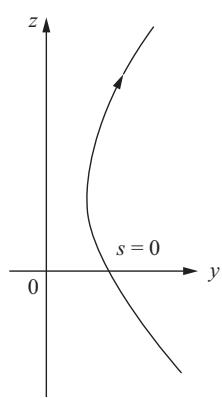
\includegraphics[width=0.45\textwidth]{../../../PDFs/differential-geometry/transcript/Do Carmo - Differential Geometry of Curves and Surfaces/hybrid_ocr/images/98f40d772f751b0834697b463c35ad7a8eea3b64812095e1e82c2a1e808dbec1.jpg}}
\subfloat[Figure 5-58(b)]{\label{fig:fig5-58b}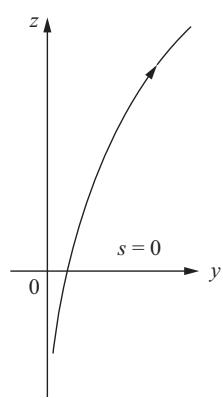
\includegraphics[width=0.45\textwidth]{../../../PDFs/differential-geometry/transcript/Do Carmo - Differential Geometry of Curves and Surfaces/hybrid_ocr/images/0b0675a867703b8fd8b714d446c3c80cc9c7c5e8feb73345a1bf9d0ea71370a3.jpg}}

\subfloat[Figure 5-58(c)]{\label{fig:fig5-58c}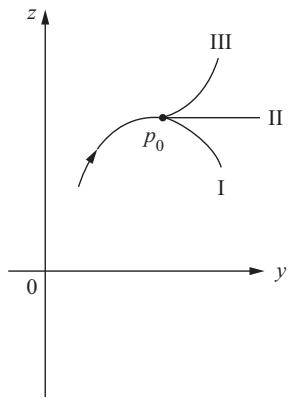
\includegraphics[width=0.6\textwidth]{../../../PDFs/differential-geometry/transcript/Do Carmo - Differential Geometry of Curves and Surfaces/hybrid_ocr/images/6e3e016f2d3b4b0520d5161b62ea9ac440ace5de8de078a69f8db919d2723357.jpg}}
\end{exercise}

\begin{exercise}{5-11, 3* — T.K. Milnor 的 Hilbert 定理证明}
设 $S$ 是带有完备度量 $g_1$ 的平面，其曲率 $K \equiv -1$。假设存在等距浸入 $\varphi \colon S \to \mathbb{R}^3$。为得到矛盾，按以下步骤进行：

a. 考虑 Gauss 映射 $N \colon \varphi(S) \subset \mathbb{R}^3 \to S^2$，并设 $g_2$ 是 $S$ 上的度量，使得 $N \circ \varphi \colon S \to S^2$ 是局部等距。在 $S$ 上选取局部坐标，使得 $\varphi$ 的坐标曲线像是 $\varphi(S)$ 的渐近曲线。证明在此坐标系中，$g_1$ 可以写成
\[
du^2 + 2\cos\theta\,dudv + dv^2,
\]
而 $g_2$ 可以写成
\[
du^2 - 2\cos\theta\,dudv + dv^2.
\]

b. 证明 $g_3 = \frac{1}{2}(g_1 + g_2)$ 是 $S$ 上具有零曲率的度量。利用 $g_1$ 是完备度量且 $3g_3 \geq g_1$，推出度量 $g_3$ 也是完备的。

c. 证明带有度量 $g_3$ 的平面整体等距于标准欧几里得平面 $\mathbb{R}^2$。因此存在等距 $\psi \colon S \to \mathbb{R}^2$。进一步证明 $\psi$ 将 $S$ 的渐近曲线（用弧长参数化）映射为 $\mathbb{R}^2$ 中用弧长参数化的矩形坐标系直线。

d. 利用 c 部分给出的 $S$ 上的整体坐标系，与正文中的 Hilbert 定理证明相同地导出矛盾。
\end{exercise}

% ==================== 附录：点集拓扑（Euclidean 空间的子集）====================
\appendix
\chapter{附录：Euclidean 空间的点集拓扑}\label{chap:topology-appendix}

本附录给出第 5 章所需的点集拓扑基本概念与定理的完整叙述。这些材料使本书对读者自洽，无需外引拓扑学知识。

\section{连通性与紧致性}

\begin{Definition}\label{def:connected}
集合 $A \subset \mathbb{R}^n$ 称为\textbf{连通的}（connected），如果它不能表示为两个非空不相交开子集的并。
\end{Definition}

\begin{Definition}\label{def:compact}
集合 $A \subset \mathbb{R}^n$ 称为\textbf{紧致的}（compact），如果它的任意开覆盖都有有限子覆盖。等价地，紧致 $\Leftrightarrow$ 有界且闭（Heine-Borel 定理）。
\end{Definition}

\begin{Proposition}\label{prop:continuous-image-compact}
紧致集在连续映射下的像是紧致的。
\end{Proposition}

\begin{Corollary}\label{coro:compact-surface}
紧致正则曲面是紧致的（作为 $\mathbb{R}^3$ 的子集）。
\end{Corollary}

\begin{Definition}\label{def:boundary}
设 $A \subset \mathbb{R}^n$，点 $p \in \mathbb{R}^n$ 称为 $A$ 的\textbf{边界点}（boundary point），如果 $p$ 的任意邻域与 $A$ 和 $\mathbb{R}^n - A$ 均相交。$A$ 的边界记为 $\mathrm{Bd}\,A$。
\end{Definition}

\begin{Proposition}\label{prop:open-closed}
正则曲面 $S \subset \mathbb{R}^3$ 是 $\mathbb{R}^3$ 中的开集。紧致正则曲面是 $\mathbb{R}^3$ 中的闭集。
\end{Proposition}

\section{弧道连通性}

\begin{Definition}\label{def:arcwise-connected}
集合 $B \subset \mathbb{R}^n$ 称为\textbf{弧道连通的}（arcwise connected），如果对任意 $p,q \in B$，存在连续映射 $\alpha: [0,1] \to B$ 使 $\alpha(0)=p$，$\alpha(1)=q$。
\end{Definition}

\begin{Proposition}\label{prop:arcwise-implies-connected}
弧道连通必连通。
\end{Proposition}

\begin{Proposition}\label{prop:open-arcwise-connected}
$\mathbb{R}^n$ 中的开集若连通则弧道连通。
\end{Proposition}

\begin{Corollary}
正则曲面（作为 $\mathbb{R}^3$ 的开子集）是弧道连通的。
\end{Corollary}

\section{同伦与单连通}

\begin{Definition}\label{def:homotopy}
设 $\alpha_0, \alpha_1: [0,l] \to B$ 是两条弧线，端点相同（同伦的基本群定义）。它们称为\textbf{同伦的}（homotopic），如果存在连续映射 $H: [0,l]\times[0,1] \to B$ 使 $H(s,0)=\alpha_0(s)$，$H(s,1)=\alpha_1(s)$，$H(0,t)$ 和 $H(l,t)$ 与 $t$ 无关。
\end{Definition}

\begin{Definition}\label{def:simply-connected-appendix}
弧道连通的 $B$ 称为\textbf{单连通的}（simply connected），如果任意闭弧线与常值弧线同伦。
\end{Definition}

\begin{Proposition}\label{prop:sphere-simply-connected}
球面 $S^2$ 是单连通的。
\end{Proposition}

\begin{Proposition}\label{prop:plane-simply-connected}
平面 $\mathbb{R}^2$ 是单连通的。
\end{Proposition}

\begin{Proposition}\label{prop:cylinder-not-simply-connected}
圆柱面不是单连通的。
\end{Proposition}

\section{Cauchy 序列与完备性}

\begin{Definition}\label{def:cauchy-sequence}
集合 $A \subset \mathbb{R}^n$ 中的序列 $\{p_k\}$ 称为\textbf{Cauchy 序列}，如果对任意 $\epsilon>0$，存在 $N$ 使 $k,l \geq N$ 时 $|p_k - p_l| < \epsilon$。
\end{Definition}

\begin{Proposition}\label{prop:compact-cauchy}
紧致集中的任意序列有收敛子序列（Cauchy 收敛原理）。
\end{Proposition}

\begin{Corollary}\label{coro:closed-criterion}
$\mathbb{R}^n$ 中序列收敛当且仅当它是 Cauchy 序列且极限点属于该集合。
\end{Corollary}

\section{几点注释}

本附录的拓扑材料是第 5 章整体定理的基础。主要使用的方式：
\begin{itemize}
  \item 连通性和紧致性用于刻画曲面的整体行为（$S$ 紧致 $\Rightarrow$ 完备等）；
  \item 弧道连通性用于定义距离（第 5-3 节）和覆叠空间的性质；
  \item 单连通性在 Hadamard 定理（第 5-6 节）中起关键作用；
  \item Cauchy 序列完备性用于证明 Hopf-Rinow 定理中的收敛性论证。
\end{itemize}

\begin{Remark}
本附录不追求拓扑学的系统叙述，而是提供证明各整体定理所需的最少拓扑知识。欲深入学习的读者可参考 Munkres 的《Topology》或 Milnor 的《Topology from the Differential Viewpoint》。
\end{Remark}
